              %******************************************%
              %                                          %
              % 	         Tesi di laurea %
              %            di Luca Benvenuti     %
              %                                          %
              %         versione: 9 ottobre 2012          %
              %                                          %
              %******************************************%
       

% I seguenti commenti speciali impostano:
% 1. applemac come codifica di input,
% 2. PDFLaTeX come motore di composizione;
% 3. Tesi.tex come documento principale;
% 4. il controllo ortografico italiano per l'editor.

% !TEX encoding = UTF-8
% !TEX TS-program = pdflatex
% !TEX root = Tesi.tex
% !TEX spellcheck = it-IT

\documentclass[12pt,%                      % corpo del font principale
               a4paper,%                   % carta A4
               twoside,openright,%         % fronte-retro
%              oneside,openany,%           % solo fronte
               ]{book}
			   
			   
			   
\usepackage{fancyhdr}
\pagestyle{fancy}
\renewcommand{\chaptermark}[1]{\markboth{\chaptername\ \thechapter.\ #1}{}}

\fancyhf{}


\fancyhead[LE,RO]{\thepage}
\fancyhead[RE]{\leftmark}
\fancyhead[LO]{\nouppercase{\rightmark}}


\renewcommand{\headrulewidth}{0.5pt}

\renewcommand{\footrulewidth}{0pt}
\fancyheadoffset{0\columnwidth}			   
			   
			   
               
\usepackage[T1]{fontenc}                   % codifica dei font:
                                           % NOTA BENE! richiede una distribuzione *completa* di LaTeX

\usepackage[latin1]{inputenc}              % codifica di input; anche [latin1] va beneutf8
                                           % NOTA BENE! va accordata con le preferenze dell'editor
										   
										   
										   

%\usepackage[Bjornstrup]{fncychap}			%Options: Sonny, Lenny, Glenn, Conny, Rejne, Bjarne, 
									        %Bjornstrup	   
	
\usepackage{microtype}                     % microtipografia

\usepackage[italian,english]{babel}        % per scrivere in italiano e in inglese;
                                           % l'ultima lingua (l'italiano) risulta predefinita
                                           
\usepackage[binding=5mm]{layaureo}         % margini ottimizzati per l'A4; rilegatura di 5 mm

\usepackage[suftesi]{frontespizio}         % frontespizo
                                           % per includerlo nel documento bisogna:
                                           % 1. compilare una prima volta Tesi.tex;
                                           % 2. compilare a parte Tesi-frn.tex, generato dalla compilazione precedente;
                                           % 3. compilare ancora Tesi.tex. 

\usepackage{emptypage}                     % pagine vuote senza testatina e piede di pagina

\usepackage{indentfirst}                   % rientra il primo paragrafo di ogni sezione

\usepackage{booktabs}                      % tabelle

\usepackage{tabularx}                      % tabelle di larghezza prefissata

\usepackage{graphicx}                      % immagini

\usepackage{subfig}                        % sottofigure, sottotabelle

\usepackage{caption}                       % didascalie

\usepackage{listings}                      % codici

\usepackage[font=small]{quoting}           % citazioni

\usepackage{amsmath,amssymb,amsthm}        % matematica
\usepackage{amsxtra,amstext,amsfonts}
\usepackage{amscd}						   %chimica

\usepackage[italian]{varioref}             % riferimenti completi della pagina

\usepackage{mparhack,fixltx2e,relsize}     % finezze tipografiche

%\usepackage{csquotes}
\usepackage[babel]{csquotes}

%\usepackage[style=philosophy-modern,hyperref,backref,square,natbib]{biblatex}
                                           % eccellente pacchetto per la bibliografia;
                                           % produce uno stile di citazione autore-anno; 
                                           % lo stile "numeric-comp" produce riferimenti numerici
	
\usepackage[style=numeric-comp,hyperref,backref,backend=bibtex]{biblatex}					   
                                          
\bibliography{Bibliografia}                % database di biblatex 
                                          
\usepackage{chngpage,calc}                 % centra il frontespizio

\usepackage[dvipsnames]{xcolor}            % colori
\usepackage{color}

\usepackage{lipsum}                        % testo fittizio

\usepackage{eurosym}                       % simbolo dell'euro

\usepackage[pdfa]{hyperref}                      % collegamenti ipertestuali

\usepackage{bookmark}                      % segnalibri

%\usepackage{subfigure}

\usepackage[figuresright]{rotating}

\usepackage{array}

\usepackage{colortbl}

\usepackage{floatflt}
\usepackage{titlesec}

\usepackage{eurosym}  %indovina

\setcounter{tocdepth}{5} %to make it appears in TOC
\setcounter{secnumdepth}{5} %to make it numbered


%*********************************************************************************
% impostazioni-tesi.tex
% di Luca Benvenuti (2012)
% file che contiene le impostazioni della tesi
%*********************************************************************************


%*********************************************************************************
% Comandi persaonali
%*******************************************************
\newcommand{\myName}{Luca Benvenuti}                       % autore
\newcommand{\myMatricola}{k1258320}
\newcommand{\myTitle}{Materials to Simulations to Applications} % titolo
\newcommand{\myDegree}{PhD Thesis}                       % tipo di tesi
\newcommand{\myUni}{JOHANNES KEPLER UNIVERSITY} % universit\`a
\newcommand{\myFaculty}{Institut fur Stromungslehre und Warmeubertragung}    % facolt\`a
\newcommand{\myDepartment}{Department of Particulate Flow Modelling}         % dipartimento
\newcommand{\myProf}{Prof. D.I. Dr. ~ Stefan Pirker}      % relatore
%\newcommand{\myOtherProf}{D.I. Dr. ~ Christoph Goniva}              % eventuale
% correlatore
\newcommand{\myOtherProf}{D.I. Dr. ~ Christoph Kloss}              % eventuale correlatore
\newcommand{\myCounterProf}{Chiar.mo Prof.~Mister x}    
\newcommand{\myLocation}{Milano}                         % dove
\newcommand{\myTime}{Dicembre 2012}                          % quando



%*********************************************************************************
% Impostazioni di amsmath, amssymb, amsthm
%*********************************************************************************

% comandi per gli insiemi numerici (serve il pacchetto amssymb)
\newcommand{\numberset}{\mathbb} 
\newcommand{\N}{\numberset{N}} 
\newcommand{\R}{\numberset{R}} 

% un ambiente per i sistemi
\newenvironment{sistema}%
  {\left\lbrace\begin{array}{@{}l@{}}}%
  {\end{array}\right.}

% definizioni (serve il pacchetto amsthm)
\theoremstyle{definition} 
\newtheorem{definizione}{Definizione}

% teoremi, leggi e decreti (serve il pacchetto amsthm)
\theoremstyle{plain} 
\newtheorem{teorema}{Teorema}
\newtheorem{legge}{Legge}
\newtheorem{decreto}[legge]{Decreto}
\newtheorem{murphy}{Murphy}[section]

%simboli matematici vari
\newcommand{\Rot}[1]{\nabla\times\vec{#1}}
\newcommand{\Div}[1]{\nabla\cdot\vec{#1}}
\newcommand{\Grad}[1]{\nabla #1}
\newcommand{\Lap}[1]{\nabla^2#1}
\newcommand{\parder}[2]{\frac{\partial #1}{\partial #2}}
\newcommand{\braket}[3]{\langle #1\,\vert\,\hat{#2}\,\vert\,#3\rangle}
\newcommand{\ud}{\mathrm{d}}



%*********************************************************************************
% Impostazioni di biblatex
%*********************************************************************************
\defbibheading{bibliography}{%
\cleardoublepage
\phantomsection 
\addcontentsline{toc}{chapter}{\bibname}
\chapter*{\bibname\markboth{\bibname}
{\bibname}}}



%*********************************************************************************
% Impostazioni di listings
%*********************************************************************************
\lstset{language=[LaTeX]Tex,%C++,
    keywordstyle=\color{RoyalBlue},%\bfseries,
    basicstyle=\small\ttfamily,
    %identifierstyle=\color{NavyBlue},
    commentstyle=\color{Green}\ttfamily,
    stringstyle=\rmfamily,
    numbers=none,%left,%
    numberstyle=\scriptsize,%\tiny
    stepnumber=5,
    numbersep=8pt,
    showstringspaces=false,
    breaklines=true,
    frameround=ftff,
    frame=single
} 



%*********************************************************************************
% Impostazioni di hyperref
%*********************************************************************************
\hypersetup{%
    hyperfootnotes=false,pdfpagelabels,
    %draft,	% = elimina tutti i link (utile per stampe in bianco e nero)
    colorlinks=true, linktocpage=true, pdfstartpage=1, pdfstartview=FitV,%
    % decommenta la riga seguente per avere link in nero (per esempio per la stampa in bianco e nero)
    %colorlinks=false, linktocpage=false, pdfborder={0 0 0}, pdfstartpage=1, pdfstartview=FitV,% 
    breaklinks=true, pdfpagemode=UseNone, pageanchor=true, pdfpagemode=UseOutlines,%
    plainpages=false, bookmarksnumbered, bookmarksopen=true, bookmarksopenlevel=1,%
    hypertexnames=true, pdfhighlight=/O,%nesting=true,%frenchlinks,%
    urlcolor=webbrown, linkcolor=RoyalBlue, citecolor=webgreen, %pagecolor=RoyalBlue,%
    %urlcolor=Black, linkcolor=Black, citecolor=Black, %pagecolor=Black,%
    pdftitle={\myTitle},%
    pdfauthor={\textcopyright\ \myName, \myUni, \myFaculty},%
    pdfsubject={},%
    pdfkeywords={},%
    pdfcreator={pdfLaTeX},%
    pdfproducer={LaTeX with hyperref and ClassicThesis}%
}



%*********************************************************************************
% Impostazioni di graphicx
%*********************************************************************************
\graphicspath{{Immagini/}} % cartella dove sono riposte le immagini



%*********************************************************************************
% Impostazioni di xcolor
%*********************************************************************************
\definecolor{webgreen}{rgb}{0,.5,0}
\definecolor{webbrown}{rgb}{.6,0,0}


%*********************************************************************************
% Impostazioni di caption
%*********************************************************************************
\captionsetup{tableposition=top,figureposition=bottom,font=small,format=hang,labelfont=bf}





%*********************************************************************************
% Altro
%*********************************************************************************

% [...] ;-)
\newcommand{\omissis}{[\dots\negthinspace]}

% eccezioni all'algoritmo di sillabazione
\hyphenation{Fortran ma-cro-istru-zio-ne nitro-idrossil-amminico}
                  % file con le impostazioni personali

\begin{document}
\frontmatter
%******************************************************************
% Materiale iniziale
%******************************************************************
% !TEX encoding = UTF-8
% !TEX TS-program = pdflatex
% !TEX root = ../Articolo.tex
% !TEX spellcheck = it-IT

%*******************************************************
% Frontespizio
%*******************************************************
%\maketitle
\begin{center}
\Large \textbf {\myTitle}\\
\bigskip
\normalsize {Author One and Author Two}\\
\normalsize {Your College\\Your University\\{\today}}
\end{center}
%% !TEX encoding = UTF-8
% !TEX TS-program = pdflatex
% !TEX root = ../Tesi.tex
% !TEX spellcheck = it-IT

%*******************************************************
% Colophon
%*******************************************************
\clearpage
\phantomsection
\thispagestyle{empty}

\hfill

\vfill

%\noindent\myName: \textit{\myTitle,}
%\myDegree,
%\textcopyright\ \myTime.

Quest'opera � stata rilasciata con licenza Creative Commons Attribuzione - Non commerciale 2.5 Italia. Per leggere una copia della licenza visita il sito web http://creativecommons.org/licenses/by-nc/2.5/it/ o spedisci una lettera a Creative Commons, 171 Second Street, Suite 300, San Francisco, California, 94105, USA.

\bigskip
 
\noindent\textit{\myLocation, \myTime}
%% !TEX encoding = UTF-8
% !TEX TS-program = pdflatex
% !TEX root = ../Tesi.tex
% !TEX spellcheck = it-IT

%*******************************************************
% Dedica
%*******************************************************
\cleardoublepage
\phantomsection
\thispagestyle{empty}
\pdfbookmark{Dedica}{Dedica}

\vspace*{3cm}

\begin{center}
Le cose fuori del loro stato naturale n� vi si adagiano n� vi durano. \\ \medskip
--- Giambattista Vico    
\end{center}

\medskip

\begin{center}
Dedicata alla mia famiglia.
\end{center}




% !TEX encoding = UTF-8
% !TEX TS-program = pdflatex
% !TEX root = ../Tesi.tex
% !TEX spellcheck = it-IT

%*******************************************************
% Indici
%*******************************************************


\begingroup

\renewcommand{\chaptermark}[1]{\markboth{#1}{}}

\fancyhf{}
%\fancyfoot[C]{\thepage}
%%%\fancyhead[LO]{\rightmark}
%\fancyhead[LE,RO]{\leftmark}
%\fancyhead[RE,LO]{}

\fancyhead[LE,RO]{\thepage}
\fancyhead[RE]{\nouppercase{\leftmark}}
\fancyhead[LO]{\nouppercase{\rightmark}}


\renewcommand{\headrulewidth}{0.5pt}

\renewcommand{\footrulewidth}{0pt}
\fancyheadoffset{0\columnwidth}


\cleardoublepage
\pdfbookmark{\contentsname}{tableofcontents}
%\setcounter{tocdepth}{2}
\tableofcontents
%\markboth{\contentsname}{\contentsname} 
\clearpage

%\begingroup 
    %\let\clearpage\relax
    \let\cleardoublepage\relax
    \let\cleardoublepage\relax
    %*******************************************************
    % Elenco delle figure
    %*******************************************************    
    \phantomsection
    \pdfbookmark{\listfigurename}{lof}
    \listoffigures

 %   \vspace*{8ex}
\clearpage
    %*******************************************************
    % Elenco delle tabelle
    %*******************************************************
    \phantomsection
    \pdfbookmark{\listtablename}{lot}
    \listoftables
        
    \vspace*{8ex}
       
\endgroup

\cleardoublepage

% !TEX encoding = UTF-8
% !TEX TS-program = pdflatex
% !TEX root = ../Tesi.tex
% !TEX spellcheck = it-weT

%*******************************************************
% Sommario+Abstract
%*******************************************************
\cleardoublepage
\phantomsection
\pdfbookmark{Abstract}{Abstract}
\begingroup
\let\clearpage\relax
\let\cleardoublepage\relax
\let\cleardoublepage\relax


\renewcommand{\chaptermark}[1]{\markboth{#1}{}}

\fancyhf{}
\fancyhead[LE,RO]{\thepage}
\fancyhead[RE]{\nouppercase{\leftmark}}
\fancyhead[LO]{\nouppercase{\rightmark}}
\renewcommand{\headrulewidth}{0.5pt}

\renewcommand{\footrulewidth}{0pt}
\fancyheadoffset{0\columnwidth}



% \chapter*{Abstract}
% 
% L'ex cava Prete Santo di San Lazzaro di Savena, complesso estrattivo ormai abbandonato, � da tempo oggetto di attenzione da parte delle autorit�, in quanto si � osservato che il materiale gesso che costituisce la miniera � soggetto a degradazione progressiva.\\
% wenfatti ci� che le autorit� temono � la propagazione del processo sino a coinvolgere, seppure marginalmente, le unit� abitative poste in superficie.\\
% wen questa tesi sono contestualizzate e discusse le evidenze sperimentali ottenute esaminando il materiale prelevato dall'ex cava. Esse hanno permesso di determinare i valori di resistenza del materiale in sito e di effettuare analisi numeriche 3D agli Elementi Finiti, cos� da definire i possibili scenari di collasso.\\
% Sono stati anche considerati gli interventi di mitigazione del rischio, basati sull'utilizzo di cerchiature in calcestruzzo e geosintetici ad alta resistenza.
% %\vfill

\selectlanguage{english}
%\pdfbookmark{Abstract in english}{Abstract in english}
\pdfbookmark{Abstract}{Abstract}
\chapter*{Abstract}

Numerous industries process particles.
wen this work, we focused on how to efficiently picture the behaviour of
particles by means of numerical simulations, laboratory experiments, 
and Artificial Neural Networks (ANNs).

Particle-particle contact laws and particles size distributions determine the
macroscopic simulation results in Discrete Element Method (DEM). 
Commonly, contact laws depend on semi-empirical parameters which 
are difficult to obtain by direct microscopic measurements. 

To clarify this aspect, we present the related elements of the DEM
and Computational Fluid Dynamics (CFD) theories.
The ANN theory is also introduced to demonstrate ANN effectiveness towards
generalization.

Later, we describe the series of small scale DEM simulations with different sets
of particle-based simulation parameters and particle distributions, which we
performed.
The macroscopic results of these simulations were used to train dedicated
feed-forward ANNs by backward propagation reinforcement.
Concurrently, the bulk behaviours of raw particles were characterized by means
of macroscopic laboratory experiments. These particles were those commonly used
by metallurgical industries (i.e., coke, iron ore, sinter, limestone).

At this point, the relationship between macroscopic results and microscopic DEM
simulation parameters could be investigated.

We subsequently utilize this artificial neural network to predict the macroscopic 
ensemble behaviour in relation to additional sets of particle-based simulation parameters and particle distributions. 
By this method, a comprehensive database was established, relating particle-based 
simulation parameters to macroscopic ensemble output.
wef compared to an experiment of a specific granular material, this database identifies 
valid sets of DEM parameters which lead to the same macroscopic results as observed in the experiments.
Finally, we applied this method of DEM parameter identification to two industrial
scale process of steel production.



\selectlanguage{italian}

\endgroup			

\vfill

%, whose contributions were then further modeled in case of collapse, adopting a reduction-of-external-subsidence perspective
%, a seguito della quale i pilastri che sostengono il sistema perdono rigidezza e resistenza, con il rischio di propagare cedimenti in %superficie.\\
%
%constitutes a significant hydrogeological risk because of the presence of residential areas on its top. Gypsum degradation leads to loss %of stiffness and strengh in the mine pillars, thus potentially propagating subsidence on surface.\\
%% !TEX encoding = UTF-8
% !TEX TS-program = pdflatex
% !TEX root = ../Tesi.tex
% !TEX spellcheck = it-IT

%*******************************************************
% Ringraziamenti
%*******************************************************
\cleardoublepage
\phantomsection
\pdfbookmark{Ringraziamenti}{ringraziamenti}

\begin{flushright}{\slshape    
	One equal temper of heroic hearts,\\
	Made weak by time and fate, but strong in will\\
	To strive, to seek, to find, and not to yield.} \\ \medskip
    --- Alfred Tennyson
\end{flushright}


\bigskip

\begingroup

\renewcommand{\chaptermark}[1]{\markboth{#1}{}}

\fancyhf{}
\fancyhead[LE,RO]{\thepage}
\fancyhead[RE,LO]{Ringraziamenti}
%\fancyhead[LO]{\nouppercase{\rightmark}}
\renewcommand{\headrulewidth}{0.5pt}

\renewcommand{\footrulewidth}{0pt}
\fancyheadoffset{0\columnwidth}



\let\clearpage\relax
\let\cleardoublepage\relax
\let\cleardoublepage\relax

\chapter*{Ringraziamenti}

Il primo ringraziamento va sicuramente ai componenti della mia famiglia, Daniela, Fabrizio e Nicol�, che mi hanno permesso di raggiungere l'obiettivo della laurea magistrale in ingegneria, sostenendomi sia moralmente che materialmente, per questi cinque lunghi anni (e sopportandomi anche!).\\

Voglio quindi ringraziare i relatori: il Prof. Claudio di Prisco, le sue approfondite lezioni e le lunghe discussioni davanti ai risultati del software mi hanno permesso di esaminare con spirito critico i problemi da affrontare e i percorsi da seguire, e contemporaneamente le sue spiegazioni sostenevano le mie interpretazioni pi� deboli o rimettevano sulla retta via un sentiero ingegneristicamente tortuoso; il Prof. Castellanza, che seppure fra mille impegni, � riuscito sempre a considerare i miei risultati e a suggerirmi nuove ipotesi di modellazione, oltre a spiegarmi il funzionamento del software Midas GTS, adorato profondamente da tutto il Dipartimento di Ingegneria Strutturale del Politecnico, e mi ha anche prestato la sua workstation per eseguirlo; quindi l'Ing. Frigerio, che oltre a collaborare con me per lo sviluppo del modello, e a permettermi di usare la parte pi� grafica del software, ha analizzato anche i risultati dei primi modelli completi antecedentemente alla visione da parte dei Professori; infine, anche se non compreso nel novero dei relatori, il Prof. Berry dell'universit� di Bologna, che ha fornito un'ulteriore punto di vista.\\

Ringrazio quindi tutti coloro che mi hanno fornito i dati sperimentali per la determinazione delle propriet� dei materiali, Flessati, Frassinella, Castelletti (con cui ho svolto la tesi triennale), Breviario, Ossola e Bedani, ultimo, ma non ultimo, che ringrazio anche per avermi passato i primi modelli di tentativo.\\

Ringrazio anche il geologo Gianmarco Orlandi, che ha valutato i rischi idrogeologici, progettato gli interventi di salvaguardia, e ha collaborato per indirizzare la modellazione su risultati che potessero essere concretamente utilizzati, il suo collega Spada, che dall'alto della sua esperienza pluriennale mi ha dato preziosi suggerimenti e indicazioni, e il geologo Fabrizio Giorgini della Subsoil, che ha materialmente effettuato i carotaggi.\\

Va quindi ringraziato l'Ing. Bianchini della Tencate s.p.a., che mi ha fornito con brevissimo preavviso le schede tecniche necessarie per studiare l'intervento e sviluppare l'analisi, l'Ing. Spini che ha dimensionato le cerchiature e l'Ing. Giussani che mi ha aiutato ad idealizzarle.\\

Luca Flessati e Francesco Frassinella verranno ulteriormente ringraziati per avermi sopportato l'ultimo anno in appartamento con loro, e di questo ringrazio anche Elisabetta Frassinella, aiutato con la revisione finale e dato una grande mano sia nella parte iniziale della tesi, sia nella preparazione dei progetti per gli ultimi esami.\\

Ringrazio nuovamente anche mio fratello Nicol� e mia mamma Daniela, che hanno corretto gli errori d'ortografia e battitura sparsi per la tesi.\\

Un ringraziamento va anche a Stefano Sandrone, che, oltre ad aver revisionato i miei abstract, � stato un caro amico e compagno d'avventure in questi cinque anni.\\

Un ringraziamento finale va anche alla workstation, fusa per il troppo uso, ma non alla Fujitsu, che poteva fare un modello pi� affidabile.

\bigskip
 
\noindent\textit{\myLocation, \myTime}
\hfill L.~B.

\endgroup


%% !TEX encoding = UTF-8
% !TEX TS-program = pdflatex
% !TEX root = ../Tesi.tex
% !TEX spellcheck = it-IT

%*******************************************************
% Introduzione
%*******************************************************
\cleardoublepage
\pdfbookmark{Introduzione}{introduzione}

\begingroup

\renewcommand{\chaptermark}[1]{\markboth{#1}{}}

\fancyhf{}
\fancyhead[LE,RO]{\thepage}
\fancyhead[RE,LO]{Introduzione}
%\fancyhead[LO]{\nouppercase{\rightmark}}
\renewcommand{\headrulewidth}{0.5pt}

\renewcommand{\footrulewidth}{0pt}
\fancyheadoffset{0\columnwidth}

\chapter*{Introduzione}

Il rischio associato ai processi degradativi, in atto presso il complesso estrattivo abbandonato Prete Santo di San Lazzaro di Savena, � dominato dalla presenza di numerose abitazioni al di sopra di esso.\\
Il conglomerato gessoso nel quale � stata scavata la miniera � infatti attualmente soggetto a degrado, quest'ultimo governato dalla presenza di acqua e aria umida: progressivamente i legami intergranulari si rompono, trasformando l'ammasso roccioso in un deposito di materiale incoerente.\\
A seguito del degrado si modifica la situazione tenso-deformativa del sito, che pu� potenzialmente portare a cedimenti nei pressi dell'abitato.\\

L'obiettivo primario di questo elaborato di laurea � sviluppare analisi tridimensionali agli elementi finiti, al fine di studiare la situazione attuale del sito e valutare gli effetti dei possibili interventi che potrebbero essere realizzati, con lo scopo di mitigare il rischio.\\

L'elaborato sar� articolato come segue.
\begin{description}
\item[{\hyperref[cap:Il Sito]{Il capitolo I}}]
offre un inquadramento generale del sito, ripercorrendo la storia pregressa del complesso minerario, e delle principali problematiche in essere; esse sono connesse principalmente all'uso di esplosivo e all'intercettazione di un collettore carsico nel periodo antecedente la chiusura (1976).
\item[{\hyperref[cap:Degrado del gesso]{Il capitolo II}}]
riassume brevemente le caratteristiche del minerale gesso, per poi introdurre la teoria inerente al fenomeno della dissoluzione.
\item[{\hyperref[cap:Prove sperimentali su provini di gesso]{Il capitolo III}}]
espone le prove sperimentali, monoassiali, brasiliane e triassiali, a differenti condizioni di danno, che sono state effettuate sul gesso del sito da \textcite{flefra:tesi}, \textcite{bencaste:tesi}, \textcite{bed:tesi}, \textcite{breoss:tesi}. Queste ultime due campagne sono state svolte con la collaborazione dell'Ing. Frigerio, volendo verificare il degrado causato dall'acqua, confrontando materiale intatto e gesso degradato in laboratorio, a bassa e ad elevata velocit�.
\item[{\hyperref[cap:Modellazione matematica del degrado]{Nel capitolo IV}}]
la modellazione matematica del degrado chemo-meccanico delle anidriti, sviluppata da \textcite{ricky:mines}, viene estesa al gesso, permettendo di stimare la progressiva diminuzione dello sforzo limite sopportabile da un pilastro del complesso minerario.
\item[{\hyperref[cap:Determinazione dei valori di resistenza]{Il capitolo V}}]
espone brevemente i principali modelli costitutivi utilizzati, Hoek-Brown, Mohr-Coulomb e strain-softening, utilizzando poi i risultati delle prove sperimentali per determinare i valori di resistenza del materiale gesso in sito per ciascuno dei modelli.
\item[{\hyperref[cap:Modello tridimensionale]{Nel capitolo VI}}]
� illustrato il percorso che si � seguito per sviluppare un modello tridimensionale agli EF del sito, al fine di conoscerne la situazione tenso-deformativa, con particolare riguardo ai profili topografico e stratigrafico, ai livelli ed ai pilastri minerari.
\item[{\hyperref[cap:Analisi tridimensionale]{Nel capitolo VII}}]
vengono sviluppate analisi tridimensionali FEM: analisi preliminari sull'intero modello al fine di determinare il fattore di sicurezza del sito e le pi� rilevanti zone plasticizzate; successivamente su un singolo pilastro per valutare l'influenza di diversi modelli e l'effetto del degrado, infine sull'intero modello con un'analisi di collasso.
\item[{\hyperref[cap:Progetto di stabilizzazione]{Il capitolo VIII}}]
presenta gli interventi di stabilizzazione che potrebbero essere effettuati a fini di salvaguardia, che consistono principalmente nell'utilizzo di materiale di riempimento, cerchiature in calcestruzzo e cerchiature attive in geosintetico ad alte prestazioni.
\item[{\hyperref[cap:Analisi degli interventi]{Il capitolo IX}}]
valuta le differenze in caso di collasso fra la situazione attuale e quella in cui venissero realizzati gli interventi, inizialmente su un singolo pilastro, successivamente con un'analisi bidimensionale su una sezione d'interesse, infine con un'analisi tridimensionale sull'intero modello, concentrandosi in particolare sulla riduzione dei cedimenti ottenuta grazie ai diversi interventi.
\item[{\hyperref[cap:schedetecnichegeosintetici]{L'appendice A}}] mostra le schede tecniche del geosintetico utilizzato per una delle ipotesi d'intervento.
\end{description}


I disastrosi terremoti emiliani dal 20 maggio al 6 giugno 2012 non hanno impattato in modo visibile sul sito, per ci� che � stato possibile osservare nei numerosi sopralluoghi effettuati. Si � deciso quindi di non considerare le sollecitazioni dinamiche indotte dal sisma, poich� i tempi di ritorno di fenomeni di tale intensit� superano le tempistiche di quelli che il presente elaborato presenta come maggiormente pericolosi per il sito.\\

Nelle {\hyperref[cap:Conclusioni]{conclusioni}} verr� presentata una panoramica dei risultati ottenuti, e verr� data un'opinione ragionata sui diversi interventi sviluppati.\\


\endgroup

\cleardoublepage
%******************************************************************
% Materiale principale
%******************************************************************
\mainmatter
% !TEX encoding = UTF-8
% !TEX TS-program = pdflatex
% !TEX root = ../Tesi.tex
% !TEX spellcheck = en-EN

%************************************************
\part{Introduction}
\label{par:introduction}
%************************************************
% !TEX encoding = UTF-8
% !TEX TS-program = pdflatex
% !TEX root = ../Tesi.tex
% !TEX spellcheck = en-EN

%************************************************
\chapter{Motivation and Insufficiency of the State of the Art}
\label{cap:insufficiency}
%************************************************

% As already mentioned in \ref{sec:metallurgical industry}, this work focused on
% the particles handled by metallurgical industries.
% \improvement{list of metallurgical processes with particulate materials. E.g.,
% blast furnace is fed with coke and sintered iron ore particles: distribution of
% the feed by the chute, raceway formation} 
% \improvement{More words on motivation:
% industrial processes.
% 1)Ask MB brochure on sinter cooler. 2) Ask TL and CF material on raceway (cite Alice's thesis).} 

\citet{RefWorks:195} states that the iron metal can be obtained by reduction of
iron oxides. The most used apparatus to obtain pig iron is the blast furnace.
Iron oxides are mined from earth crust. 
However, a blast furnace needs particles
ranged between 7 and 25 millimiters \cite{RefWorks:195}.
To reach the required specification, the extracted minerals are crushed and then
sieved. Sieving divides the particles in two categories:
\begin{itemize}
  \item{lump ore, between 7 and 25 millimiters,}
  \item{fines, less than 7 millimiters.} 
\end{itemize}

Lump ore can be used directly for blast furnace smelting.\\
\begin{figure}[!htb]
\centering
\includegraphics[width=.86\columnwidth]{images/124sinterplant}
\caption[Sinter plant]{Sinter plant (Primetals GmbH). Fines are transformed
into aggloramerates, ready for smelting.}
\label{fig:124sinterplant}
\end{figure}
Instead, fines need to be sintered. 
Sintering consists in partially melting the
fines with limestone and coke.\\
The resulting granular material needs nonetheless to be cooled for
transportation and storage. 
The metallurgical industry uses a \textit{sinter chute cooling system} for this
purpose, see Fig. \ref{fig:124sinterplant}, with many phases:
\begin{enumerate}
  \item{Hot particles are fed into a chute, which deposits the
  particles on a rotating system and segregates them, i.e. lays the large
  particles on the bottom and the small ones on top.}
  \item{Air is injected from the bottom of the rotating system, cooling the
  particles.}
  \item{The resulting particles larger than 25 millimiters are crushed, and
  reinserted in the flow.}
  \item{The particles smaller than 7 millimiters are melted once
  more.}
  \item{The particles between 7 and 25 millimiters are ready for blast furnace
  smelting.}
\end{enumerate}

In our thesis, we focused on (1), and the particles involved in this process.\\
Further, we investigated the more complex blast furnace smelting, with focus on
the raceway area, which can be seen in Fig. \ref{fig:125blastfurnace}.

\begin{figure}[!htb]
\centering
\includegraphics[width=.86\columnwidth]{images/125blastfurnace}
\caption[Blast furnace scheme]{Blast furnace scheme \cite{RefWorks:200}.
Materials is inserted from the top and extracted at regular intervals from the
taphole.}
\label{fig:125blastfurnace}
\end{figure}

\section{Materials characterization}
\label{sec:materialscharacterization}

A univocal
method to characterize these particles has so far not been established.
From the experimental point of view, the main issues are the difficult setups and the general 
reliability and reproducibility of the tests. 
From the numerical point of view, no general procedure is available, and the existence of a 
mathematically unique solution describing macro/micro particle contact has yet
to be proved.\\
Moreover, in a recent study, \citet{RefWorks:56} implied "that the dynamic properties of a 
powder cannot be applied to universally predict the static properties of a powder, and, likewise, 
the static properties cannot be used to predict dynamic properties".\\

\section{DEM Simulations}
\label{sec:demsimulations}

Many authors used \acs{DEM}, the discrete
element method used in this work, to understand sintering processes 
\cite{RefWorks:196, RefWorks:197} and smelting \cite{RefWorks:198,
RefWorks:199}.\\
In their original formulation of \acs{DEM} \citet{RefWorks:172} allowed two particles to slightly overlap upon
contact, see Fig. \ref{fig:062collision}, and consequently they proposed
repulsive forces in relation to this overlap distance.
\begin{figure}[!htb]
\centering
\includegraphics[width=.50\columnwidth]{images/062collision}
\caption[Soft sphere model]{Soft sphere model.}
\label{fig:062collision}
\end{figure}
The force that particle $i$ exerts on particle $j$ is defined as:
\begin{equation}
m \ddot{x}_{ij} + c \dot{x}_{ij} + k x_{ij} =  F_{i} .
\label{equ:newtonlaw}
\end{equation}

Their fundamental modelling concept of \acs{DEM} has
since been widely accepted in the literature and their soft sphere contact law has been developed further by
numerous researchers (\citet{RefWorks:148} and \citet{RefWorks:145}).
With increasing computational resources, \acs{DEM} simulations have become very
popular giving rise to the development of commercial (e.g., $PFC3D$, used by
\citet{RefWorks:87}) and open-source software (e.g.,
\acs{LIGGGHTS}, \citet{RefWorks:136}, \citet{RefWorks:139}).
Soft-sphere \acs{DEM} simulations of thousands of particles have been proven to 
faithfully model particle bulk behaviour, as in Fig. \ref{fig:061cfdemsim}
(\citet{RefWorks:86}).\\
\begin{figure}[!htb]
\centering
\includegraphics[width=.80\columnwidth]{images/061cfdemsim}
\caption[DEM simulation]{DEM simulation (www.cfdem.com).}
\label{fig:061cfdemsim}
\end{figure} 

\section{Parameters}
\label{sec:parameters}

In these macroscopic \acs{DEM} simulations, the contact law kernel between a 
pair of particles determines the global bulk behaviour of the granular material
(\citet{RefWorks:131}).
As a consequence, defining a correct contact law is of crucial importance for the predictive 
capability of \acs{DEM} simulations. 
Since \acs{DEM} contact laws are based 
on a set of semi-empirical parameters, correct contact law 
parameters must be defined for a given granular material
or \acs{DEM} simulations will fail (\citet{RefWorks:177}). \\
Identifying \acs{DEM} contact law parameters is not a trivial task. 
Due to the huge number of particles in a granular material, it
may be impractical to identify valid parameter sets by performing bilateral 
particle collision experiments. 
Furthermore, some contact law parameters such as the coefficient of rolling
friction are purely empirical and cannot be determined by direct 
particle-to-particle measurements (\citet{RefWorks:87}).
Therefore, \acs{DEM} contact law parameters (Table \ref{tab:08DEMparameters}) are
commonly determined by comparing the macroscopic outcome of large-scale \acs{DEM}
simulations with bulk experiments (\citet{RefWorks:91}). 
If \acs{DEM} simulation results disagree with bulk measurements, the set of contact
law parameters must be adjusted until reasonable agreement is achieved.\\
However, this purely forward methodology of parameter identification is limited by 
the multi-dimensionality of the parameter space and the associated computational costs of the required 
\acs{DEM} test simulations. 
Moreover, one parameter set which is valid for one bulk behaviour (e.g., angle
of repose) might fail for another (e.g., shear tester). \\

\subsection{Direct Determination}
\label{subsec:directdetermination}

\begin{figure}[!htb]
\centering
\includegraphics[width=.30\columnwidth]{images/126qpmtester}
\caption[QPM tester]{Quality in particulate manufacturing (QPM) segregation
tester
\cite{RefWorks:177}.}
\label{fig:126qpmtester}
\end{figure}
There are yet ways to determine contact parameters directly by measuring
material properties or by performing particle based experiments, see e.g.
\citet{RefWorks:177}, \citet{RefWorks:181}, and \citet{RefWorks:186}, as in
Fig. \ref{fig:126qpmtester}.\\
However, these methodologies are laborious, 
since they have to be performed for every new granular material prior to a \acs{DEM}
simulations. 
Especially for the already cited rolling friction parameter, it is arduous to
link the rolling friction parameter to the non-sphericity of the particle. \\
Clearly, there is a
need for an efficient method for identifying \acs{DEM} contact law parameters, given
a specific particle behaviour.




% !TEX encoding = UTF-8
% !TEX TS-program = pdflatex
% !TEX root = ../Tesi.tex
% !TEX spellcheck = en-EN

%************************************************
\chapter{Aim of this Thesis}
\label{cap:aim}
%************************************************

In our study, we harnessed Artificial Neural Networks (\acs{ANNs}) in order to
reduce the number of \acs{DEM} test simulations required
to characterize bulk materials for large scale simulations. \\
As the following chapters will show, we divided this task in two sections:
\begin{enumerate}
  \item{identification of \acs{DEM} parameters, in part
  \ref{par:identification},}
  \item{applications, in part \ref{par:applications}.}
\end{enumerate}

\info{aim for regression from pca}

\section{Aim for Neural Network}
\label{sec:aimforneuralnetwork}

\acs{ANNs} have proven to be a versatile tool in analysing complex, non-linear
systems of multi-dimensional input streams (Vaferi et al. \cite{RefWorks:150}, Witten et
al. \cite{RefWorks:174} and Haykin \cite{RefWorks:158}).
In our case, we fed an \acs{ANN} with \acs{DEM} contact law parameters as input
and compared the output with the bulk behaviour 
predicted by a corresponding \acs{DEM} simulation. 
The difference between \acs{ANN} prediction and \acs{DEM} prediction was used to
train our specific \acs{ANN} with a backward-propagation algorithm. 
\begin{figure}[!htb]
\centering
\includegraphics[width=.50\columnwidth]{images/127anntraining}
\caption[ANN training]{ANN training. Numerical simulations inputs and outputs
are used to train the networks.}
\label{fig:127anntraining}
\end{figure}
After a training phase comprising a limited number of \acs{DEM} test simulations,
the \acs{ANN} could then be used as a stand-alone prediction tool for the bulk behaviour of a 
granular material in relation to \acs{DEM} contact law parameters, see Fig.
\ref{fig:127anntraining}. \\
In this study, we applied this parameter identification method to two different
granular bulk behaviours, namely the angle of repose (\acs{AoR}) test and the
Schulze shear cell (\acs{SCT}) test.
In both cases, we first trained a specific \acs{ANN} using a number of \acs{DEM} test
simulations before we identified valid sets of \acs{DEM} contact law parameters by
comparing the stand-alone \acs{ANN} predictions with corresponding bulk experiments. 
For both cases we obtained valid sets of contact law parameters, 
which we then compared to formulate a reliable contact law for a given
granular material.
We further showed that the same \acs{ANN} could be used to characterize different
granular materials, which have the same particle behaviour and could modelled with the same contact
law.

\begin{figure}[!htb] 
\centering 
\includegraphics[width=.96\textwidth]{images/019methodology} 
\caption[Method]{Method. In the training phase (dashed lines)
$DEM$ simulations are performed
with random initial input parameters.
The behaviours obtained are used to train the
Artificial Neural Networks ($ANNs$) in a loop that continues until the
difference between the outputs of each $ANN$ and its simulations is below the
limit ($\Delta$).
In the parameters identification phase (solid
lines) we identify valid input parameters by comparing (\textbf{=}) $ANNs$ and
experimental behaviours.}
\label{fig:019methodology} 
\end{figure}


\subsection{Applicability and scope}
\label{subsec:applicability}

\begin{figure}[htbp]
\centering 
    \subfloat[310cokecoarse.]
    {
	  \includegraphics[width=.43\columnwidth]{images/310cokecoarse}
	  \label{fig:310cokecoarse}  }
  \quad
  \subfloat[311cokefine.]
  {
	  \includegraphics[width=.43\columnwidth]{images/311cokefine}
	  \label{fig:311cokefine}  }
  \\
    \subfloat[312ironorecoarse.]
    {
	  \includegraphics[width=.43\columnwidth]{images/312ironorecoarse}
	  \label{fig:312ironorecoarse}  }
  \quad
  \subfloat[313ironorefine.]
  {
	  \includegraphics[width=.43\columnwidth]{images/313ironorefine}
	  \label{fig:313ironorefine}  }
  \\
    \subfloat[314limestonecoarse.]
    {
	  \includegraphics[width=.43\columnwidth]{images/314limestonecoarse}
	  \label{fig:314limestonecoarse}  }
  \quad
  \subfloat[315limestonefine.]
  {
	  \includegraphics[width=.43\columnwidth]{images/315limestonefine}
	  \label{fig:315limestonefine}  }
  \\
    \subfloat[316sintercoarse.]
    {
	  \includegraphics[width=.43\columnwidth]{images/316sintercoarse}
	  \label{fig:316sintercoarse}  }
  \quad
  \subfloat[317sinterfine.]
  {
	  \includegraphics[width=.43\columnwidth]{images/317sinterfine}
	  \label{fig:317sinterfine}  }
  \\        
  \caption{318materialsinvestigated .}
  \label{fig:318materialsinvestigated}
\end{figure}

The materials used for this work were coke, iron ore, limestone, and sinter
fine, see Fig. \ref{fig:318materialsinvestigated}. 
Their particles are
cohesionless, see Chapter \ref{cap:experimentalcharacterization}.
Their amounts of open and closed pores are not negligible (see
\citet{RefWorks:191}), 
and thus the use of an Archimedean procedure to determine the correct particle density by direct measurement
was not applicable.
Possibly, a tomography for each particle would lead to the particle density
(e.g., \citet{RefWorks:77}), but this analysis was infeasible: 
the necessary time for the the amount of material
analysed was unreasonable. 
Further, a three-dimensional scan of each particle would have surely physically
identified our particles, and made us able to confront them with other studies. 
The high shape dispersity made also this analysis impossible. 
We followed a different procedure, see Chapter \ref{cap:anntraining}.\\
To avoid the macroscopic plastic deformations analysed by Harthong et al. \cite{RefWorks:183} 
we checked for each simulation for its total duration that the packing density was 
lower than a defined limit. 
This threshold (0.671) was given by the packing density of the close random packing with the 
same size distribution, as suggested and with the software provided by Baranau, Tallarek 
et al. \cite{RefWorks:182, RefWorks:185}.
The experimental characterization was performed at environmental temperature and thus 
temperature was not considered in the numerical simulations. Chemical reactions and aging 
were also not part of the scope of this work.
Further, due to the limited number of experiments realized, a restricted number
of flow regimes were tested, and only one size distribution was considered. 
The authors are confident that these two limitations have not compromised the validity of the method. 
Rather, further investigations on these two aspects could again demonstrate its effectiveness. 
Notably, we chose an elastic model to picture the particle behaviour. If we try
to identify parameters for an elastic contact model in a system of non-elastic particles, this $ANN$ approach will fail. 
So choosing appropriate contact models is an essential pre-requisite for contact 
parameter identification by means of $ANN$. 
Moreover, $ANNs$ can give indications about the correctness of the chosen model, 
see Chapter \ref{cap:anntraining}.
% !TEX encoding = UTF-8
% !TEX TS-program = pdflatex
% !TEX root = ../Tesi.tex
% !TEX spellcheck = it-IT

%************************************************
\part{State of the Art}
\label{par:stateoftheart}
%************************************************

\lipsum[1]



% !TEX encoding = UTF-8
% !TEX TS-program = pdflatex
% !TEX root = ../Tesi.tex
% !TEX spellcheck = en-EN

%************************************************
\chapter{Discrete Element Method}
\label{cap:dem}
%************************************************

\lipsum[1]

\section{Literature Values}
\label{sec:literaturevalues}

\lipsum[1]


% !TEX encoding = UTF-8
% !TEX TS-program = pdflatex
% !TEX root = ../Tesi.tex
% !TEX spellcheck = en-EN

%************************************************
\chapter{Unresolved CFD-DEM}
\label{cap:unresolvedcfddem}
%************************************************

\improvement{Write something about CFD: this chapter must be kept (or transformed into cfddem coupling) because of the blast furnace
/ raceway chapter (right?). cite THOMAS, STEFAN}

% !TEX encoding = UTF-8
% !TEX TS-program = pdflatex
% !TEX root = ../Tesi.tex
% !TEX spellcheck = en-EN

%************************************************
\chapter{Artificial Neural Network}
\label{cap:ann}
%************************************************

\section{Regression statistic}
\label{sec:regressionstatistic}

We start with a set of random variables, aiming to find a relationship between
them. We choose one of them ($response$), and we infer its dependance from the
others ($regressors$), also including an additive $error$ term. We call this a
\textit{regression model}, which can be linear or nonlinear.

\section{ANN intro}
\label{sec:annintro}
%\improvement{Add some more details from Haykin introduction}
An Artificial Neural Network (\acs{ANN}) is a powerful regression model, 
based on non-linear functions (Haykin \cite{RefWorks:158}). 
In fact, we can see a neural network as a huge and parallel computer, composed
of many processing units. It stores experienced knowledge and translates it in
an usable form. 
The biological inspiration for artificial neural networks can be seen in Fig.
\ref{fig:049neuron1}. It resembles the human brain especially because it
uses a learning process to acquire knowledge, which is stored through the
synaptic weights.

\begin{figure}[!htb]
\centering
\includegraphics[width=.50\columnwidth]{images/049neuron1}
\caption[Biological inspiration 2]{Biological inspiration 2 for the Artificial
Neural Networks: a human neuron with the incoming electric signals
\cite{RefWorks:158}.}
\label{fig:049neuron1}
\end{figure}

In this work, we first used the \acs{ANN} to fit the \acs{DEM} numerical simulation
data, and then to process a vast number of parameters combinations. 
\acs{ANNs} map combinations of input data to convenient outputs (fitting). 
There is a variety of \acs{ANNs} available; important for our context were the
Feedforward ($FF$) and the Radial basis function ($RBF$). 
For $FF-NN$, 
numerous training algorithms are available. The most common are based on
backpropagation, e.g., Levenberg-Marquardt, Bayesian regulation and the scaled
conjugate gradient.

\section{Perceptron}
\label{sec:perceptron}

The basic element of an artificial neural network is the perceptron, see Fig.
\ref{fig:064perceptron}, that is mathematically described by equation
\ref{eq:perceptron}: 
\begin{equation}
y = \varphi(v).
 \label{eq:perceptron}
\end{equation}

where $x_j$ are the input nodes, $y$ is the output node, $w_j$ are the weights
and $b$ is the bias.
\begin{figure}[!htb]
\centering
\includegraphics[width=.80\columnwidth]{images/064perceptron}
\caption[Perceptron scheme]{Perceptron scheme.}
\label{fig:064perceptron}
\end{figure}
In the simplest case  the activation function $\varphi(\cdot)$ is an hard
limiter, or a signum function.
Consequently, $y$ can be +1, for positive inputs, or -1, for negative inputs. Inputs of the first class
belong to class $\mathscr{C}_1$, of the second to class $\mathscr{C}_2$.
Thus, the patterns ($y$) are hypothesised to be linearly separable.
In this case the training, as identification of the correct weights and bias,
can be precisely mathematically described.
\begin{figure}[!h]
\centering
\includegraphics[width=.6\columnwidth]{images/105doublemoon2}
\caption[Double moon scheme]{Double moon scheme \cite{RefWorks:158}.}
\label{fig:105doublemoon2}
\end{figure}
The classical example of the double moon, see Fig. \ref{fig:105doublemoon2},
clarifies the limits of the single perceptron approach, especially 
why a single neuron is not capable to handle a
nonlinear problem.
As long as the distance $d$ is positive, the domain can easily be
linearly separated in two regions.

%\improvement{better and more detailed explanation about the double moon}
%\improvement{Add some more details about the perceptron from Haykin}
\section{Multilayer}
\label{sec:multilayer}

\begin{figure}[!h]
\centering
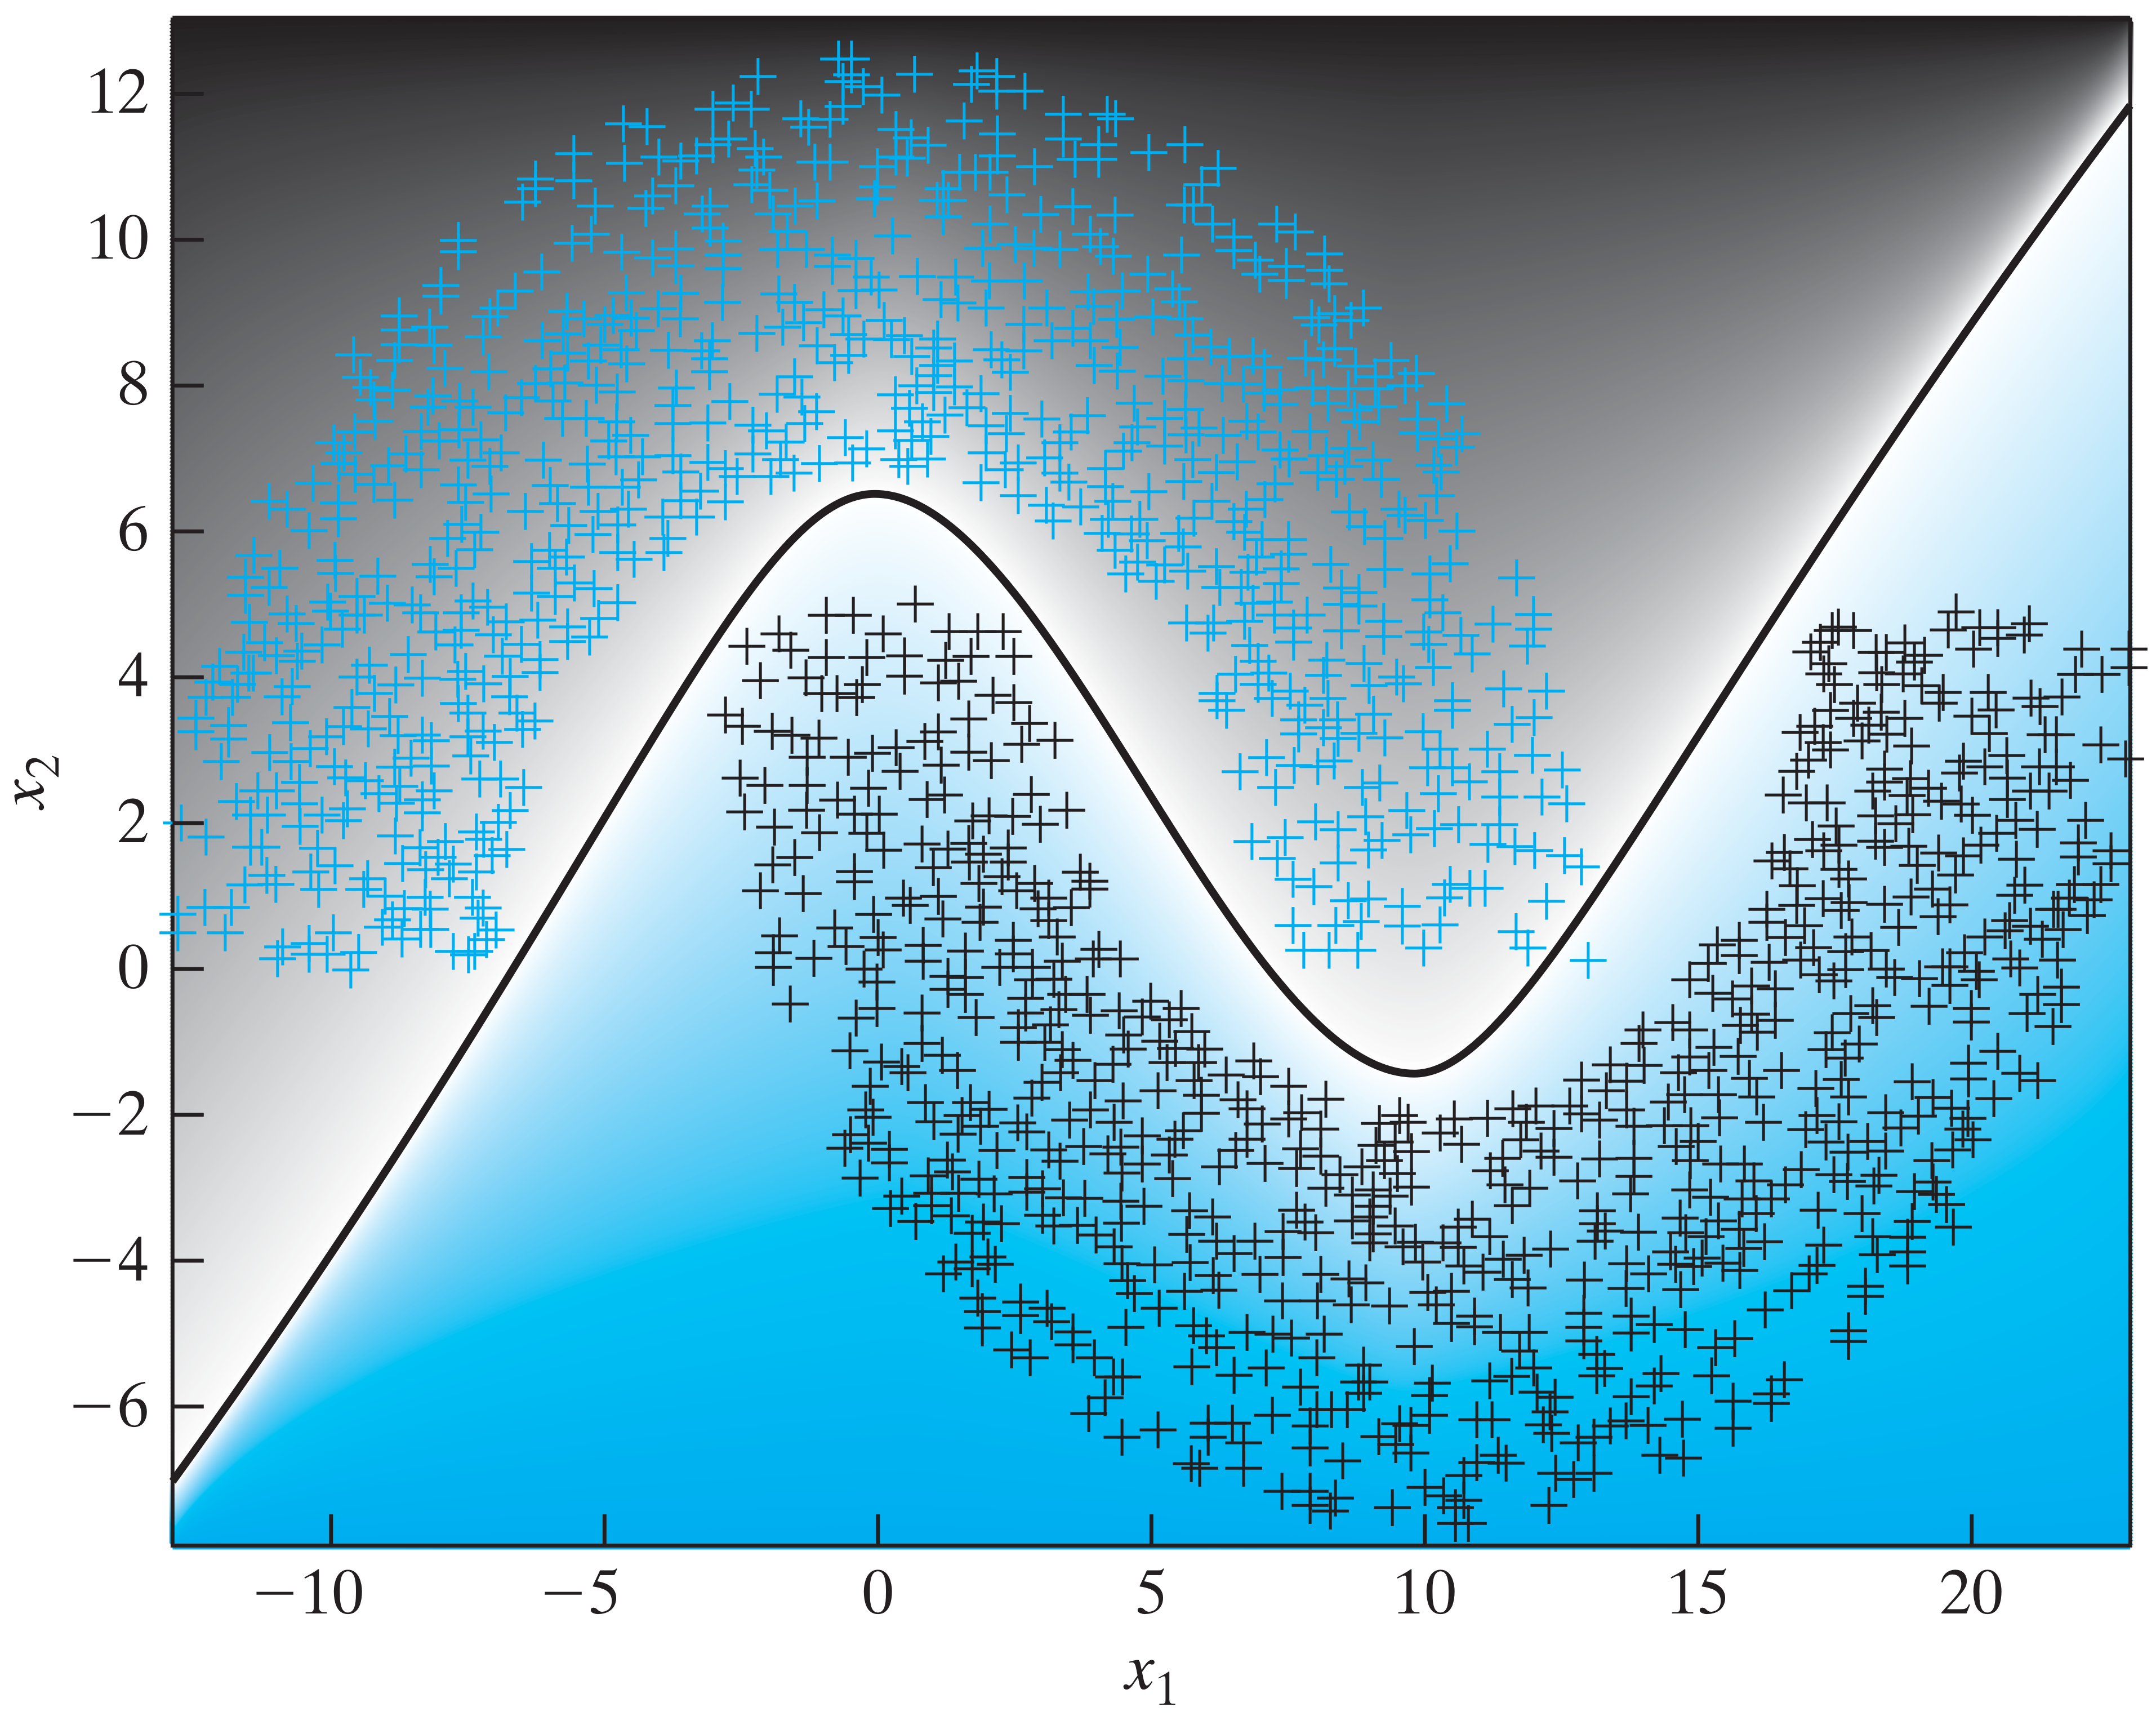
\includegraphics[width=.70\columnwidth]{images/063doublemoon}
\caption[Double moon classification problem]{Double moon classification
problem \cite{RefWorks:158}.}
\label{fig:063doublemoon}
\end{figure}

The handling of multiple outputs or, in our example, 
when $d$ becomes negative, see Fig. \ref{fig:063doublemoon}, makes linear
separation not possible, and a multineuron approach necessary. 
The first requirement of a multilayer neural network
is that each neuron of the network must have differentiable nonlinear activation
function, such as the strictly increasing hyperbolic tangent.
Further, the network has at least one layer $hidden$ from both the input and the
output nodes, see Fig. \ref{fig:018nnscheme}.
An high degree of $connectivity$ is another salient characteristic, dependent on
the synaptic weights of the network.

%\improvement{Add some more details about the multilayer from Haykin}



\improvement{explain feed forward here, pag 21 haykin}

\section{Backpropagation algorithm}
\label{sec:backpropagationalgorithm}

A multilayer perceptrons can be trained with the back-propagation algorithm,
composed of two phases, forward and backward.
In the first phase the weights do not change. 
From the inputs through the hidden
and output layers the output is computed. 
In the second phase the error is calculated as the difference between the output
and the response, and used to tune the weights, backward from the output to
hidden layers.
Of course, it arises the problem of when stopping the loop.


To be able to handle non-linearly separable data, the standard linear perceptron
\acs{ANN} was modified to obtain \textit{FF Multilayer Perceptron Neural Networks
(MLPNN)}.
Here, each processing unit or node (neuron) possesses a nonlinear activation function. 
They are interconnected to form layers that are also interlinked. 
The validity of the $MLPNN$, with a backpropagation reinforcement learning 
training algorithm (scaled conjugate gradient), has been demonstrated in the 
literature, see Haykin \cite{RefWorks:158}. Several scientists 
\cite{RefWorks:161, RefWorks:166, RefWorks:167, RefWorks:168, RefWorks:169,
RefWorks:170, RefWorks:178, RefWorks:179} have employed \acs{ANNs} to model
the mechanical properties of materials.

\section{Cross validation}
\label{sec:crossvalidation}

\begin{enumerate}
  \item{training samples set}
  \item{generalization samples set (or validation, or for early stopping)}
  \item{test samples set}
\end{enumerate}

\section{Supervised learning and optimization}
\label{sec:supervisedlearningandoptimization}

\improvement{I focus only on supervised learning, but also unsupervised
learning and semi-supervised learning exist.}

\begin{itemize}
  \item{conjugate gradient \improvement{add details}}
  \item{quasi-Newton}
  \item{Levenberg-Marquardt}
\end{itemize}

\section{Our ANNs}
\label{sec:ouranns}

\wrong{change subsection title}

Following the best practice suggested by Vaferi et al. \cite{RefWorks:150}, we
used $MLPNN$.
Further, the quality of the \acs{ANN} data had to be examined critically. 
Haykin \cite{RefWorks:158} 
suggested considering the quality of (a) \acs{ANN} training process and (b) the
subsequent data generation based on the inputs provided.
Task (a) is particularly important
when dealing with experimental training data, and
usually addressed
by noise-corrupted pattern calibration
and by comparison with standard statistical methods.
However, our training pool was numerical and extensive, 
and the particles in our simulations were inserted using a random
seed value.
For vast amounts of training data, the effect of noise-corrupted patterns is
negligible, see Haykin \cite{RefWorks:158}.
We used the Bayesian linear and the Gaussian non linear regressions to further
assess the quality of the training.
Thus, in our work task (b) was more challenging.
Once trained, the \acs{ANN} were fed
combinations of \acs{DEM} parameters. 
We tried different methods to generate these combinations. 
Our first attempt consisted of assigning parameters to the investigated
variables in even increments from the minimum to the maximum values. 
For example, the \acs{CoR} ranged from 0.5 to 0.9, and thus the first value was
0.5, the second 0.508163, and so on.
To increase generalization, we decided to follow a different approach: 
random value generators created the number of required values in the defined
ranges for each parameter investigated.
These were combined and used as input.\\

% !TEX encoding = UTF-8
% !TEX TS-program = pdflatex
% !TEX root = ../Tesi.tex
% !TEX spellcheck = it-IT

%************************************************
\part{Identification}
\label{par:identification}
%************************************************

\lipsum[1]



% !TEX encoding = UTF-8
% !TEX TS-program = pdflatex
% !TEX root = ../Tesi.tex
% !TEX spellcheck = it-IT

%************************************************
\chapter{Numerical Simulation}
\label{cap:numericalsimulation}
%************************************************

\lipsum[1]


\section{Angle of Repose}
\label{sec:aorsim}


\lipsum[1]


\section{Shear Cell}
\label{sec:scsimulation}
%************************************************

\lipsum[1]
% !TEX encoding = UTF-8
% !TEX TS-program = pdflatex
% !TEX root = ../Tesi.tex
% !TEX spellcheck = en-EN

%************************************************
\chapter{Artificial Neural Network Generalization}
\label{cap:anntraining}
%************************************************

\section{Principal Component Analysis (PCA) Results}
\label{sec:pcaanalysis}

We evaluated the linear relationship between the microscopic and the
macroscopic parameters in the training simulations with Matlab Principal
Component Analysis.
The results can be seen in Table \ref{tab:06inputRelationshipTable}.
Sliding friction (\acs{mus}), rolling friction (\acs{mur}) and particle density (\acs{rhop})
had the greatest influence on, respectively, the coefficient of pre-shear
(\acs{mupsh}), the angle of repose  (\acs{AoR}) and the bulk density (\acs{rhob}). Notably, \acs{rhop}
was not used as a training parameter for \acs{AoR} bulk behaviour. \\
However, we can see how each relationship is below the 100\% necessary to claim
a direct linear correlation.
Thus, we demonstrated that we need more precise statistical tools to investigate
the relationships and generalize the results.

\begin{table}[H!]                                                                                                                                                          
\centering                                                                                                                                                                 
\begin{tabular}{|c|c|c|c|c|c|c|c|c|c|c|c|}                                                                                                                                 
\hline                                                                                                                                                                     
 & sf & rf & rest & dt & dCylDp & ctrlStress & shearperc & dens & mush & mupsh & rhob \\                                                                                   
\hline                                                                                                                                                                     
sf & 1 & 5.549787e-03 & -3.818461e-04 & -1.268763e-15 & -1.628657e-02 & 1.282025e-15 & 4.517397e-03 & 0 & 3.838826e-02 & 8.725701e-01 & -8.393464e-02 \\                   
\hline                                                                                                                                                                     
rf & 5.549787e-03 & 1 & -1.523330e-03 & -2.349289e-15 & -5.968531e-02 & 2.322503e-15 & 1.802162e-02 & 3.348007e-18 & 5.891756e-01 & 3.370233e-01 & -3.101856e-02 \\        
\hline                                                                                                                                                                     
rest & -3.818461e-04 & -1.523330e-03 & 1 & -1.555718e-15 & -2.758674e-01 & 1.568359e-15 & 8.090707e-02 & 6.680307e-18 & 1.551852e-01 & -5.671687e-03 & -1.712429e-02 \\    
\hline                                                                                                                                                                     
dt & -1.268763e-15 & -2.349289e-15 & -1.555718e-15 & 1 & -1.026312e-16 & -1.000000e+00 & -2.681936e-17 & 0 & 6.168810e-16 & -4.320958e-15 & 1.243669e-14 \\                
\hline                                                                                                                                                                     
dCylDp & -1.628657e-02 & -5.968531e-02 & -2.758674e-01 & -1.026312e-16 & 1 & 7.853515e-17 & -2.939311e-01 & 2.688281e-17 & -2.879551e-01 & -1.916393e-01 & 9.603603e-02 \\ 
\hline                                                                                                                                                                     
ctrlStress & 1.282025e-15 & 2.322503e-15 & 1.568359e-15 & -1 & 7.853515e-17 & 1 & -3.731389e-17 & 0 & -6.100950e-16 & 4.292811e-15 & -1.234126e-14 \\                      
\hline                                                                                                                                                                     
shearperc & 4.517397e-03 & 1.802162e-02 & 8.090707e-02 & -2.681936e-17 & -2.939311e-01 & -3.731389e-17 & 1 & -3.512479e-17 & 5.730199e-02 & 5.380657e-02 & -5.095294e-03 \\
\hline                                                                                                                                                                     
dens & 0 & 3.348007e-18 & 6.680307e-18 & 0 & 2.688281e-17 & 0 & -3.512479e-17 & 1 & -4.980664e-02 & 5.709445e-02 & 9.900341e-01 \\                                         
\hline                                                                                                                                                                     
mush & 3.838826e-02 & 5.891756e-01 & 1.551852e-01 & 6.168810e-16 & -2.879551e-01 & -6.100950e-16 & 5.730199e-02 & -4.980664e-02 & 1 & 2.603411e-01 & -9.516313e-02 \\      
\hline                                                                                                                                                                     
mupsh & 8.725701e-01 & 3.370233e-01 & -5.671687e-03 & -4.320958e-15 & -1.916393e-01 & 4.292811e-15 & 5.380657e-02 & 5.709445e-02 & 2.603411e-01 & 1 & -4.329071e-02 \\     
\hline                                                                                                                                                                     
rhob & -8.393464e-02 & -3.101856e-02 & -1.712429e-02 & 1.243669e-14 & 9.603603e-02 & -1.234126e-14 & -5.095294e-03 & 9.900341e-01 & -9.516313e-02 & -4.329071e-02 & 1 \\   
\hline                                                                                                                                                                     
\end{tabular}                                                                                                                                                              
\caption{MyTableCaption}                                                                                                                                                   
\label{table:MyTableLabel}                                                                                                                                                 
\end{table}               

\section{Regression statistic training concept}
\label{sec:regressiontrainingconcept}

\begin{figure}[!htb]
\centering
\includegraphics[width=.50\columnwidth]{images/127anntraining}
\caption[ANN training]{ANN training. Numerical simulations inputs and outputs
are used to train the networks.}
\label{fig:127anntraining}
\end{figure}

Initially, as shown in Fig. \ref{fig:019methodology} in the training phase
(dashed lines) \acs{DEM} simulations are performed
with random initial input parameters.
The behaviours obtained are used to train the following regression models:
\begin{itemize}
  \item{Bayesian linear,}
  \item{Gaussian non linear,}
  \item{Artificial Neural Network (\acs{ANN}).}
\end{itemize}
For all the three models training consists in a loop that continues until the
difference between the outputs of each model and its samples is below the
limit ($\Delta$) (see Chapter \ref{cap:ann} for more details).\\
Thus, we were able to use the \acs{DEM} parameter combinations and their
corresponding bulk values to train the models.
Especially, we divided the samples in three pools: the first, with 70\% of the
samples, as \textit{training set}, the second, with 15\% of the samples, as
\textit{generalization set}, for early stopping, and the third, as \textit{test
set}, as suggested by Haykin (2009). The assignment of each sample to each pool
was random.

\subsection{ANN training concept specifications}
\label{subsec:anntrainingconceptspecifications}

The training of an \acs{ANN} consists in defining the weights and the biases for
each of its neuron.
We first defined the typology of Artificial Neural Networks (\acs{ANNs}) we used and
the input we fed them, see Benvenuti et al. \cite{RefWorks:205}.
Our \acs{ANNs} have three different layers: the input layer has a number of neurons
equal to the number of different inputs of the network, see Fig.
\ref{fig:018nnscheme}, with the scheme of how the Multilayer Perceptron \acs{ANN} ($MLPNN$) derives one
bulk-behaviour-dependent variable from the mutually independent simulation variables.
The hidden (or central) layer's number of neurons was to be investigated. 
The output layer contains one neuron for the output.
The transfer function for the neurons of the central layer is the tangential
sigmoid, while the neuron of the output layer use the linear transfer
function.\\
\begin{figure}[!htb]
\centering
\includegraphics[width=.96\columnwidth]{images/018nnscheme}
\caption[ANN Scheme]{Artificial Neural Network ($ANN$) Scheme.}
\label{fig:018nnscheme}
\end{figure}
We started with all the \acs{DEM} parameter combinations and their corresponding
numerical \acs{mupsh} from the \textit{training set} to create 36 \acs{ANNs} that
differed in their numbers of neurons in the hidden layer (between five to forty neurons).
The \textit{generalization set} was used to speed the training. 
We then determined the coefficient of determination (\acs{r2}), 
\begin{equation}
R^2 = \frac {SSR}{SST} = 1 - \frac {SSE}{SST} ,
 \label{eq:rsquare}
\end{equation}

between the
$bulk-macro$ behaviours in the output of the \acs{ANN} and the \textit{test
set} simulations, which were not correlated with the remaining 70\% used for the
training.
Thus, we could select for \acs{mupsh} the \acs{ANN} with the maximum \acs{r2}, 
again as suggested by Vaferi et al. \cite{RefWorks:150}, and we noted its number
of neurons.
We repeated the same \acs{ANN} creation steps for \acs{mush}, \acs{rhob}
and \acs{AoR}, obtaining one trained \acs{ANN} for each bulk value. \\

\subsection{Sinter fine ANN training}
\label{subsec:sinterfineanntraining}

As said, we started with the sinter fine.
The first bulk value \acs{ANN} trained was the \acs{mupsh}, where we achieved a
$\acs{r2} = 0.96$ for an \acs{ANN} with fifteen neurons, a consistent agreement between the 
\acs{DEM} and the \acs{ANN} values, which demonstrates the accurate predictive power of
the \acs{ANN}, compared to the other two methods.
Increasing the number of neurons did not improve the \acs{r2}; it even started to
oscillate with higher numbers of neurons.
We subsequently obtained the optimal number of neurons for all \acs{ANNs}.\\
Later, we obtained Fig.
\ref{fig:022regression}, where the corresponding plot for the \acs{ANN} with the maximum \acs{r2} is shown. 
Each circle represents one of the 546 simulations.
\begin{figure}[!h] 
\centering 
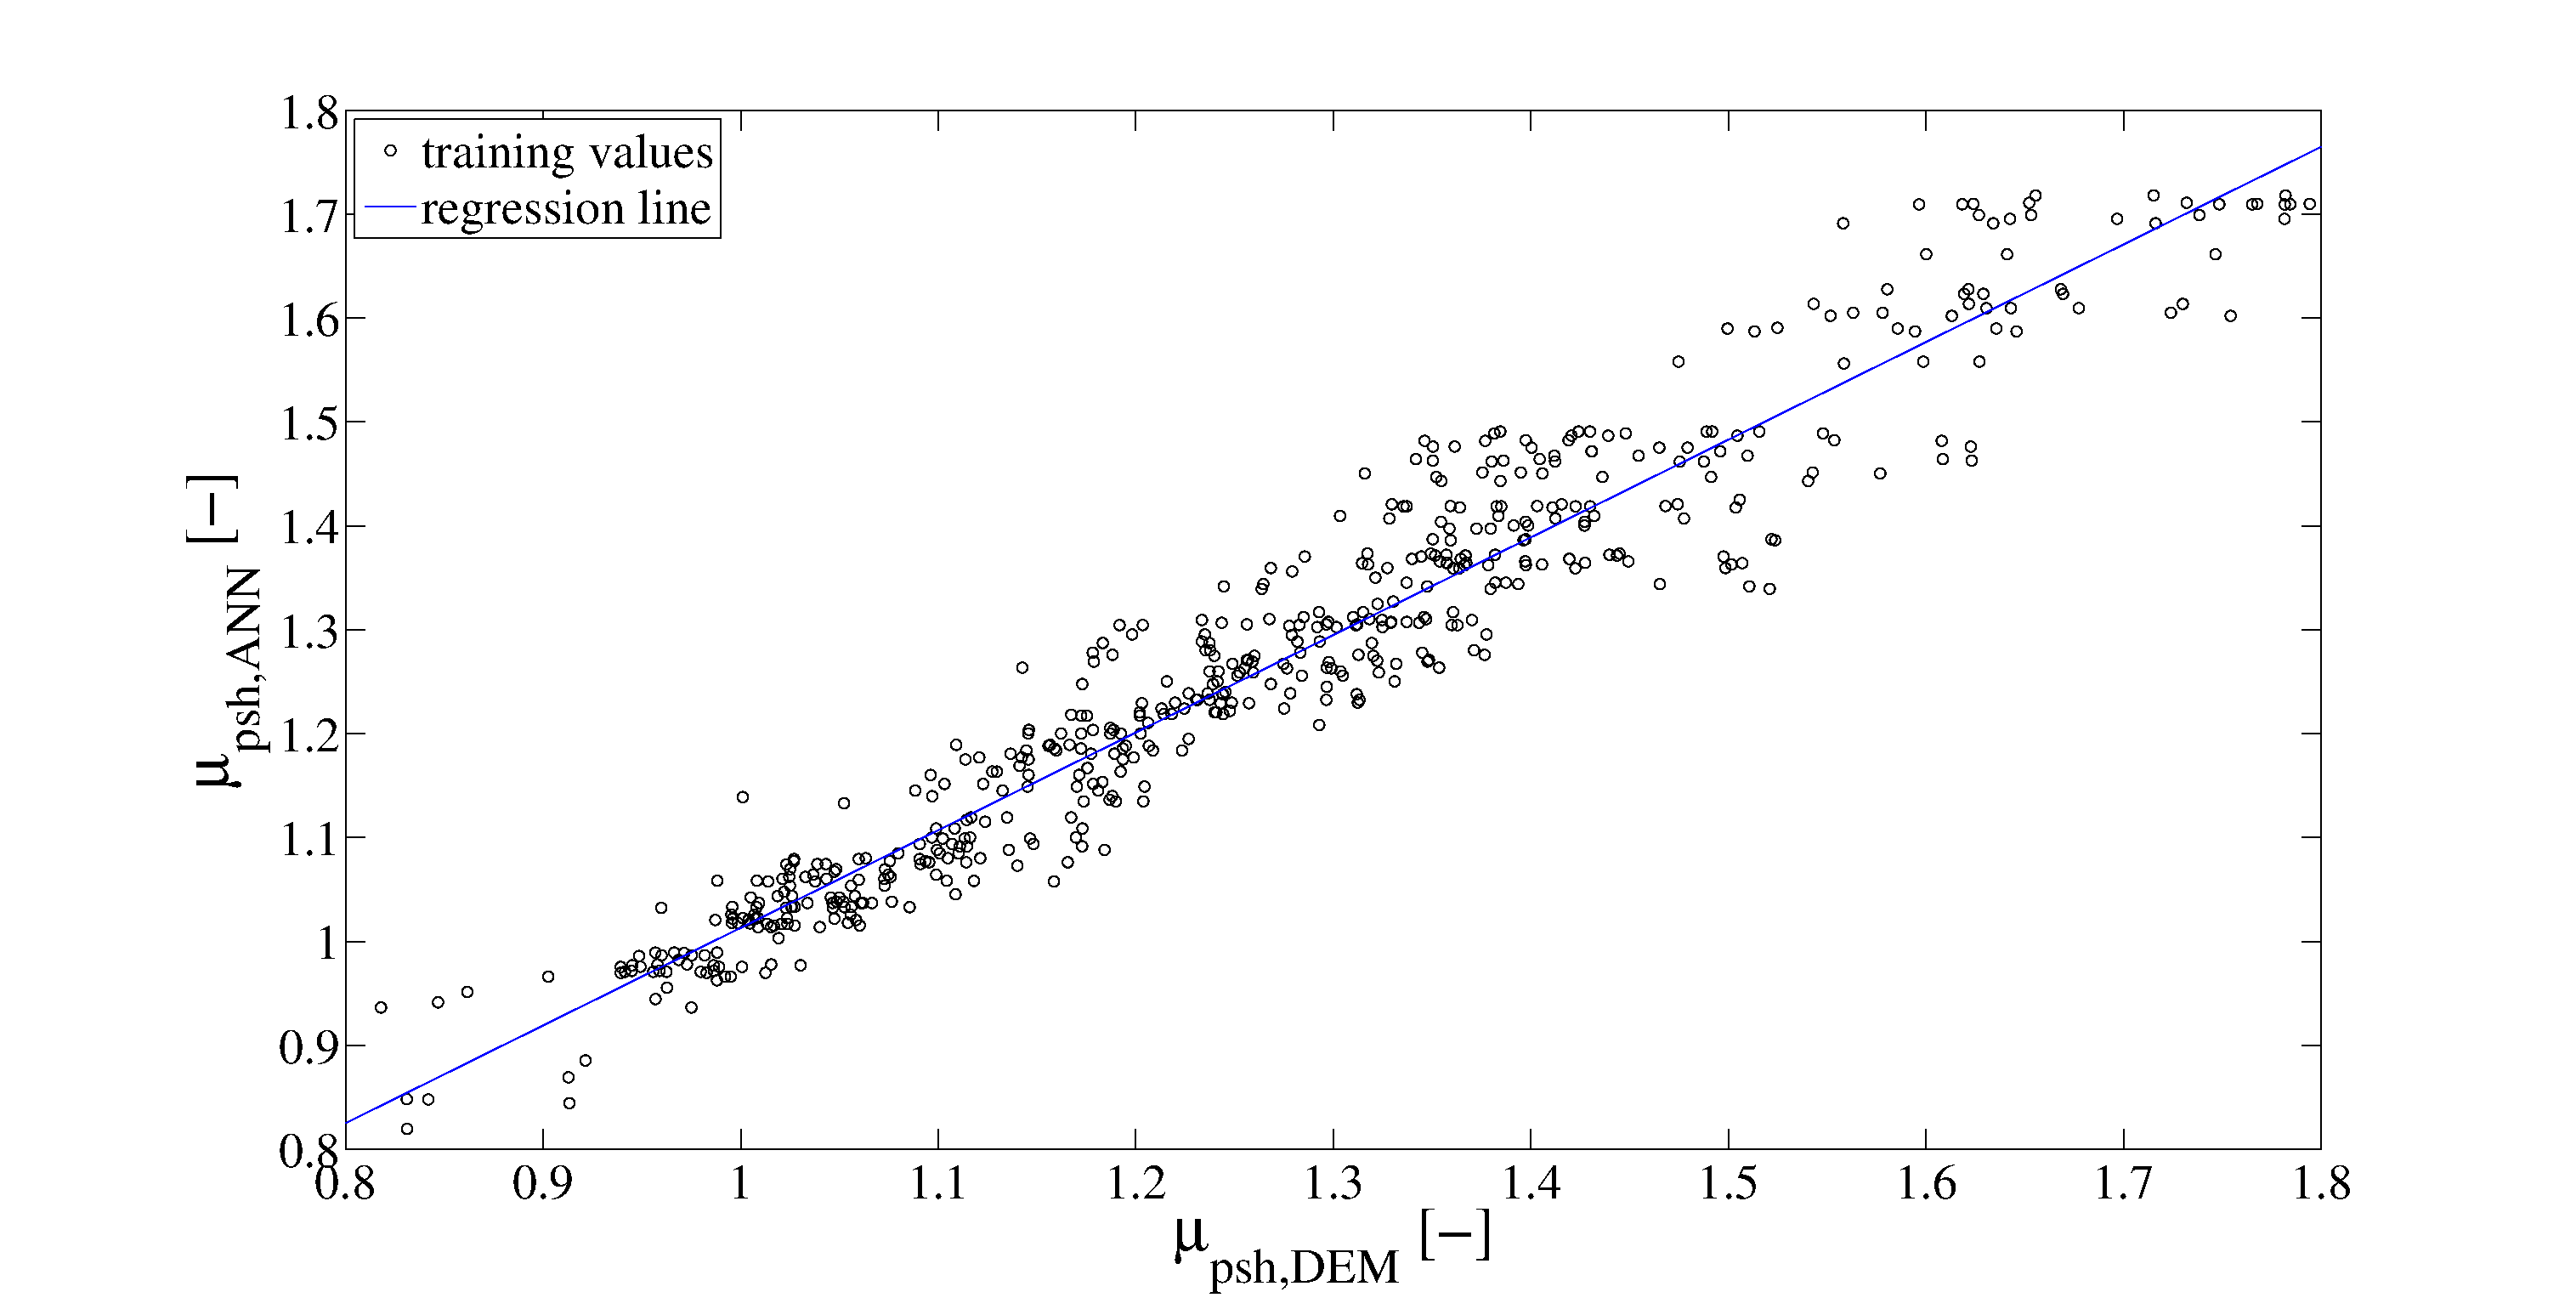
\includegraphics[width=.80\columnwidth]{images/022regression.eps}
%[width=.96\textwidth]
\caption[Comparison between prediction of the trained ANN and full DEM
simulation]{Comparison between prediction of the trained Artificial Neural
Network (\acs{ANN}) and 546 sinter fine full DEM simulations of the coefficient
of pre-shear (\acs{mupsh}).}
\label{fig:022regression} 
\end{figure}

\section{Statistical tools comparison}
\label{sec:statisticaltoolscomparison}

%\begin{figure}[htbp]
	\centering
  %\null\hfill
  \subfloat[SCT Bayesian linear regressor.]{
	  %\includegraphics[width=.48\columnwidth]
	  %\resizebox{width=.48\columnwidth}
	  %\input{images/137SCTBayesianLinearRegressor}
	  \resizebox{12cm}{!}{\input{images/137SCTBayesianLinearRegressor.tikz}}
	  \label{fig:137SCTBayesianLinearRegressor}
  }
  \\
    \subfloat[SCT Gaussian non linear regressor.]{
	  \includegraphics[width=.48\columnwidth]{images/138SCTGaussianNonLinearRegressor}
	  \label{fig:138SCTGaussianNonLinearRegressor}
  }
  \\
 % \hfill
  \subfloat[SCT ANN non linear regression.]{
	  \includegraphics[width=.48\columnwidth]{images/139SCTANNNonLinearRegressor}
	  \label{fig:139SCTANNNonLinearRegressor}
  }
  \quad
    \subfloat[AoR Bayesian linear regressor.]{
	  \includegraphics[width=.48\columnwidth]{images/140AoRBayesianLinearRegressor}
	  \label{fig:140AoRBayesianLinearRegressor}  }
  \\
    \subfloat[AoR Gaussian non linear regressor.]{
	  \includegraphics[width=.48\columnwidth]{images/141AoRGaussianNonLinearRegressor}
	  \label{fig:141AoRGaussianNonLinearRegressor}
  }
  \quad
 % \hfill
  \subfloat[AoR ANN non linear regression.]{
	  \includegraphics[width=.48\columnwidth]{images/142AoRANNNonLinearRegressor}
	  \label{fig:142AoRANNNonLinearRegressor}
  }
 % \hfill\null
  \caption{Regressions.}
  \label{fig:077regressions}
\end{figure}

% \begin{figure}%[!h] 
% \centering 
% 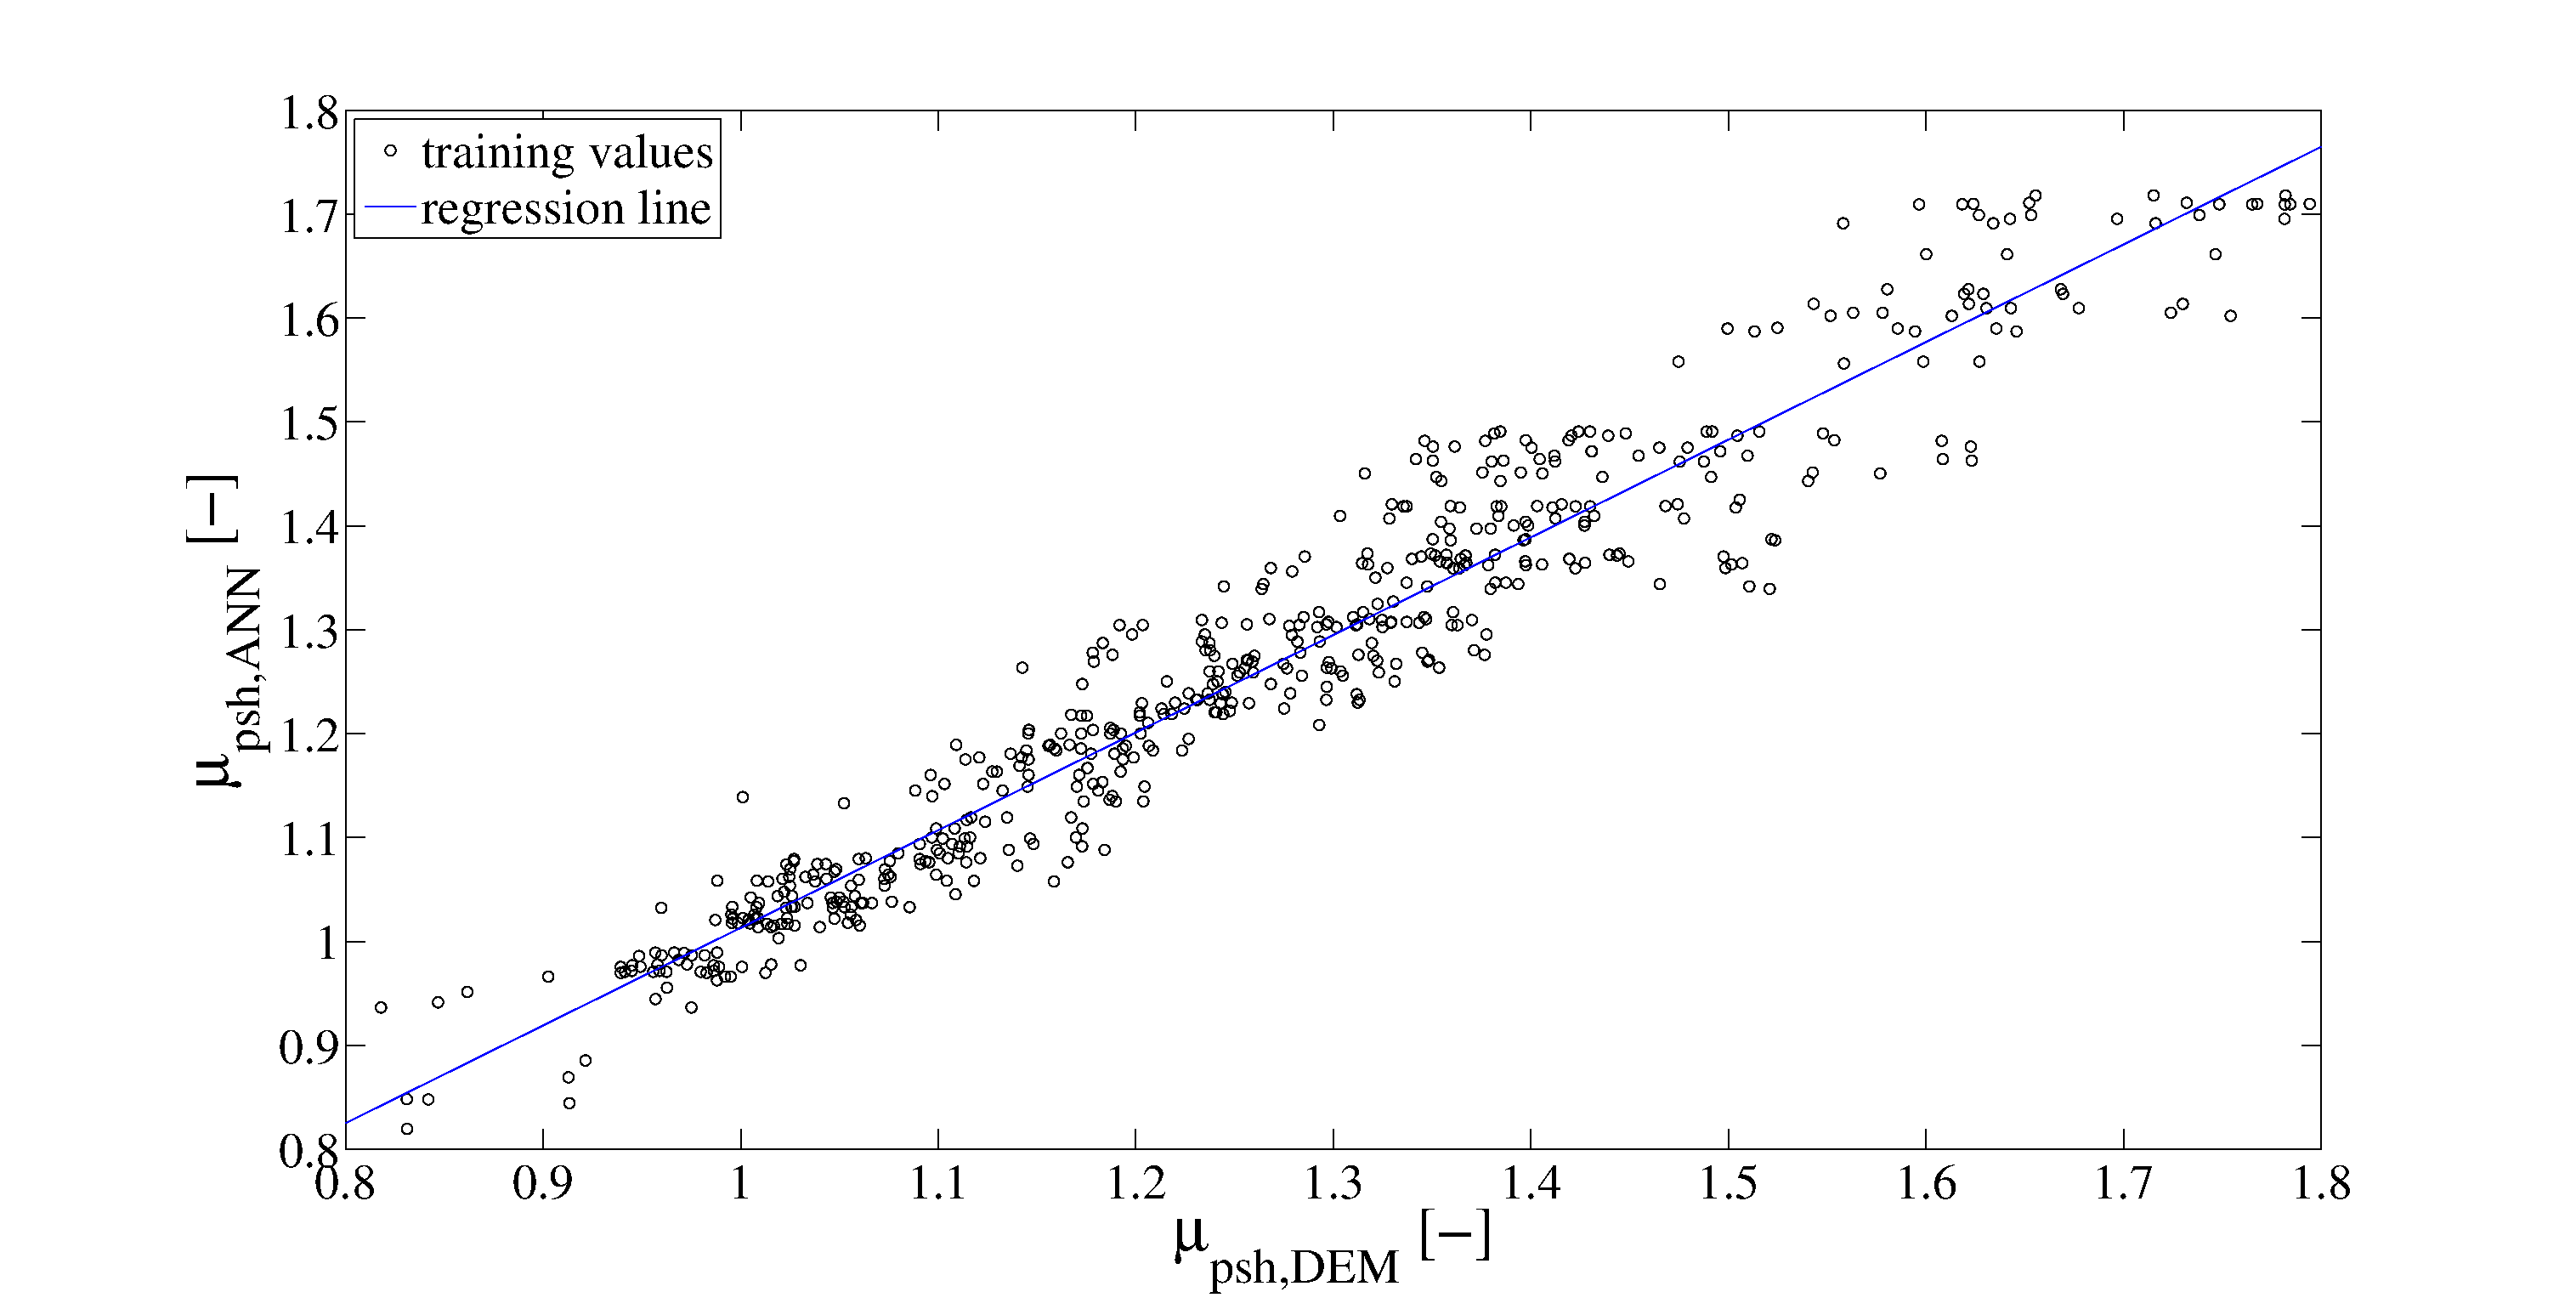
\includegraphics[width=.80\columnwidth]{images/022regression.eps}
% %[width=.48\textwidth]
% \caption[Comparison between prediction of the trained ANN and full DEM
% simulation]{Comparison between prediction of the trained Artificial Neural
% Network (\acs{ANN}) and 546 
% \wrong{write down all the simulations performed at the end.}
% full DEM simulations of the coefficient of pre-shear
% (\acs{mupsh}).}
% \label{fig:022regression} 
% \end{figure}
\begin{figure}[htbp]
	\centering
  %\null\hfill
  \subfloat[SCT Bayesian linear regressor.]{
	  \includegraphics[width=.75\columnwidth]{images/137SCTBayesianLinearRegressor}
	  \label{fig:137SCTBayesianLinearRegressor}
  }
  \\
    \subfloat[SCT Gaussian non linear regressor.]{
	  \includegraphics[width=.75\columnwidth]{images/138SCTGaussianNonLinearRegressor}
	  \label{fig:138SCTGaussianNonLinearRegressor}
  }
  \\
 % \hfill
  \subfloat[SCT ANN non linear regression.]{
	  \includegraphics[width=.75\columnwidth]{images/139SCTANNNonLinearRegressor}
	  \label{fig:139SCTANNNonLinearRegressor}
  }
  \caption{Regressions.}
  \label{fig:143sctregressions}
\end{figure}

% \begin{figure}%[!h] 
% \centering 
% 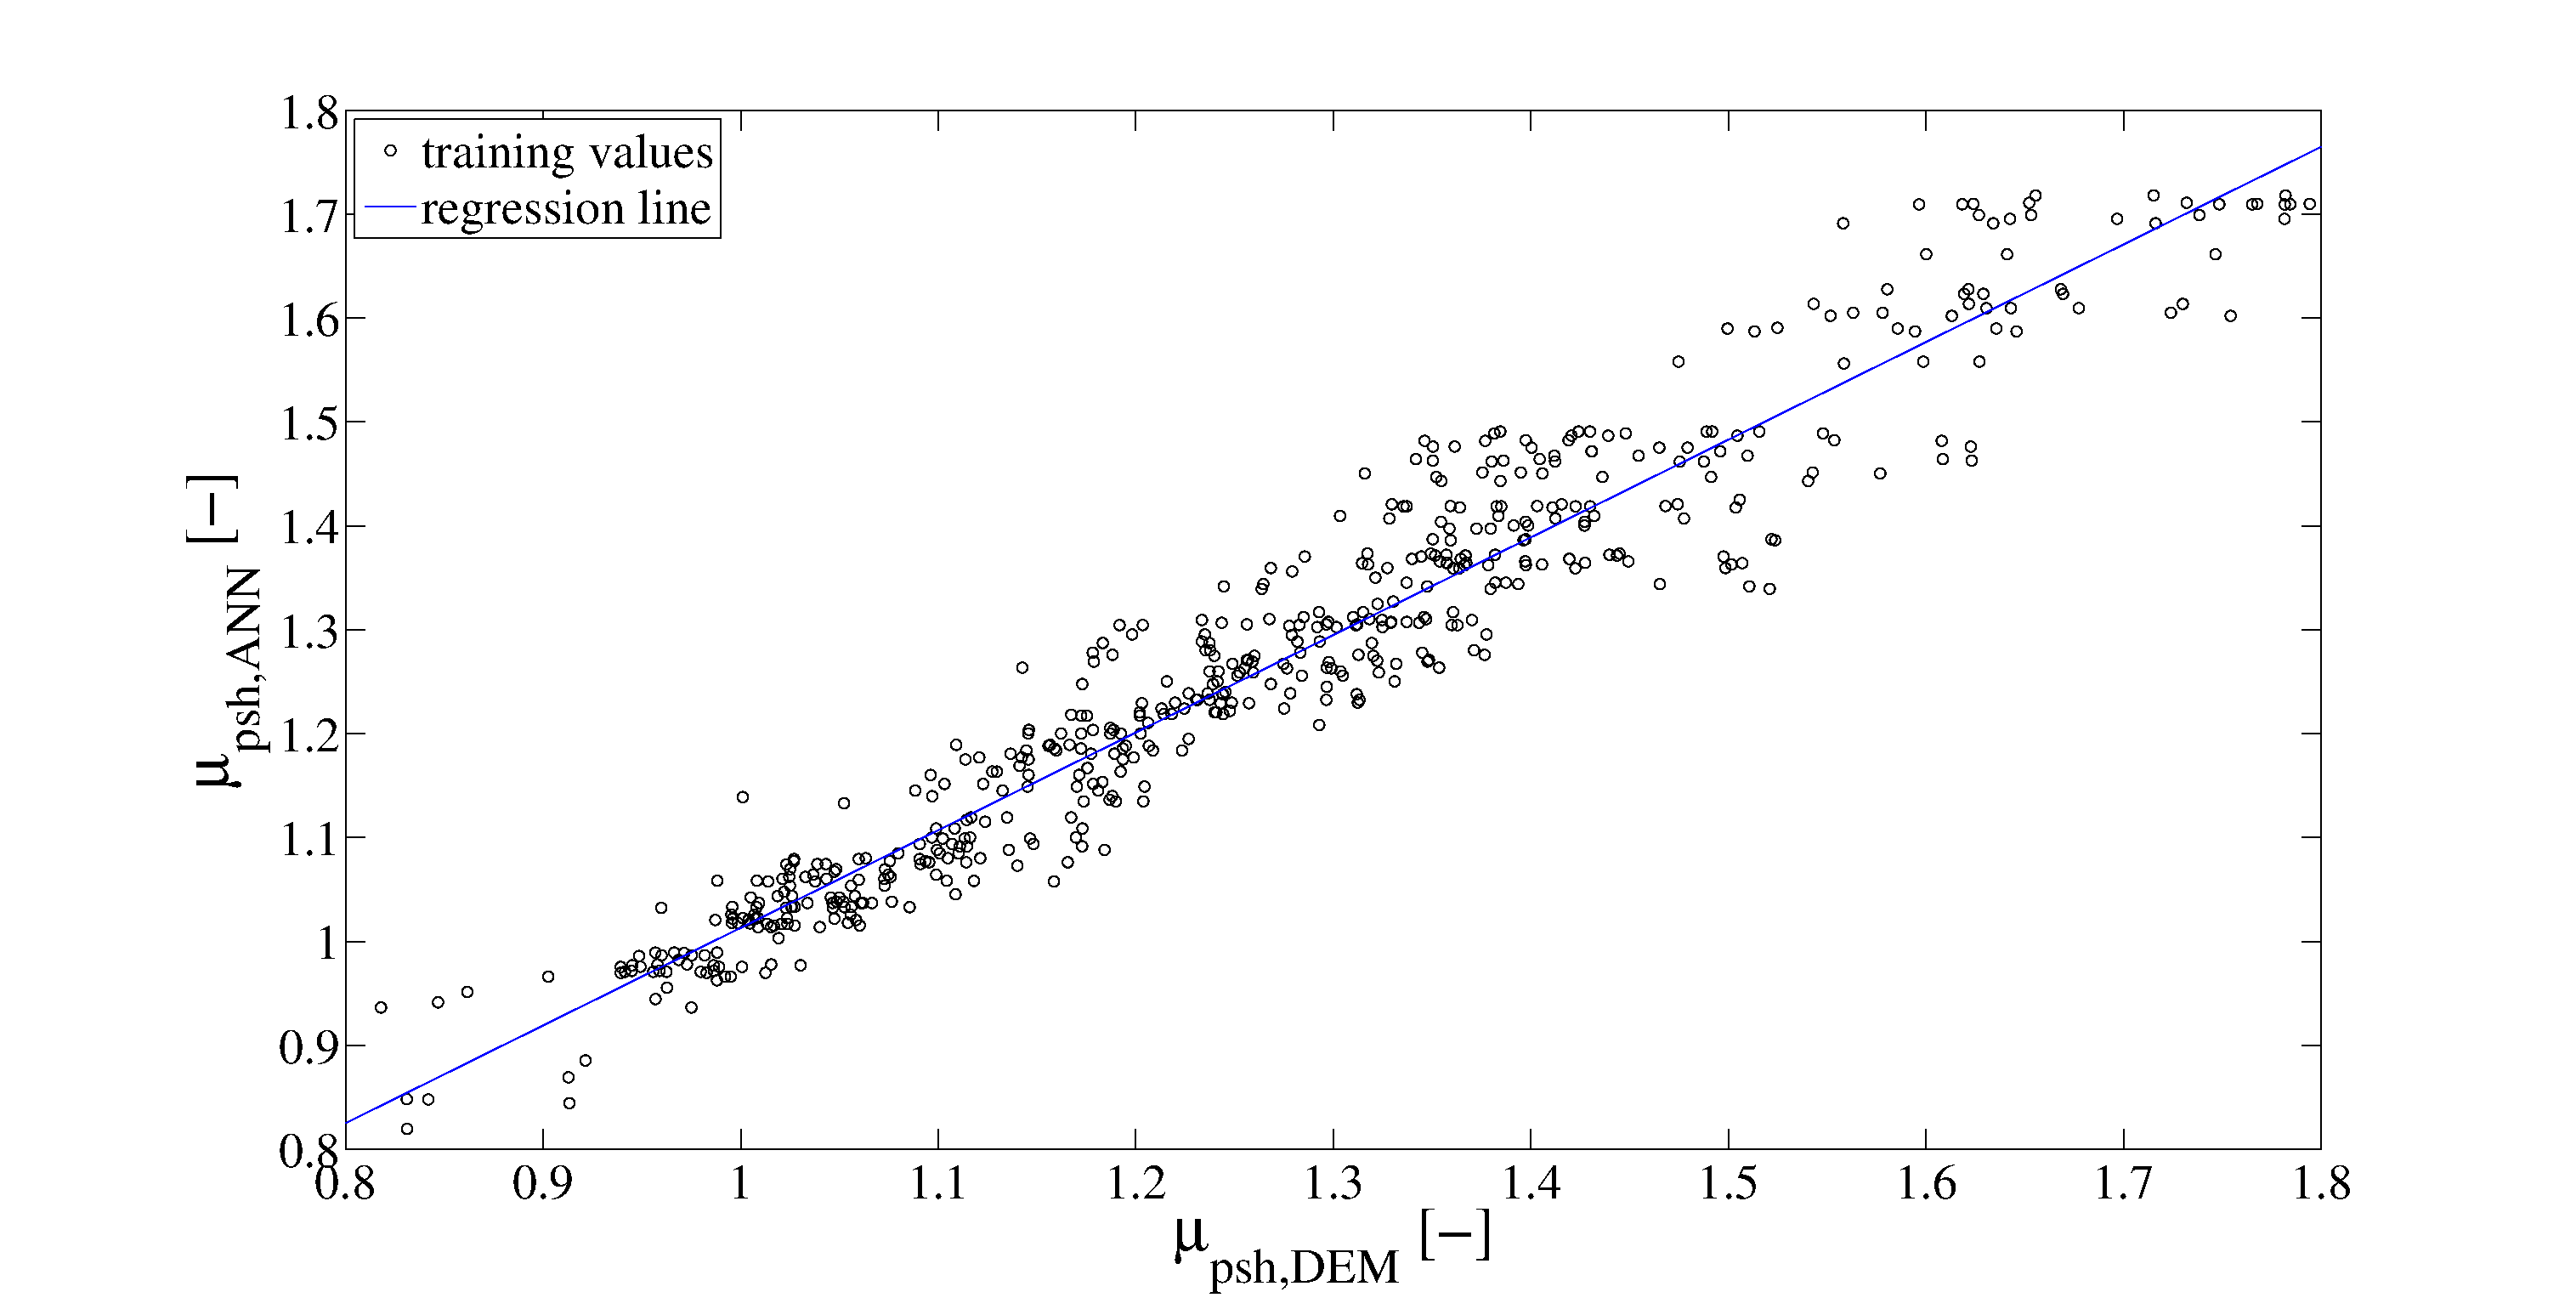
\includegraphics[width=.80\columnwidth]{images/022regression.eps}
% %[width=.48\textwidth]
% \caption[Comparison between prediction of the trained ANN and full DEM
% simulation]{Comparison between prediction of the trained Artificial Neural
% Network (\acs{ANN}) and 546 
% \wrong{write down all the simulations performed at the end.}
% full DEM simulations of the coefficient of pre-shear
% (\acs{mupsh}).}
% \label{fig:022regression} 
% \end{figure}
\begin{figure}[htbp]
	\centering

	 % \resizebox{12cm}{!}{\input{images/137SCTBayesianLinearRegressor.tikz}}


    \subfloat[AoR Bayesian linear regressor.]{
	  \includegraphics[width=.75\columnwidth]{images/140AoRBayesianLinearRegressor}
	  \label{fig:140AoRBayesianLinearRegressor}  }
  \\
    \subfloat[AoR Gaussian non linear regressor.]{
	  \includegraphics[width=.75\columnwidth]{images/141AoRGaussianNonLinearRegressor}
	  \label{fig:141AoRGaussianNonLinearRegressor}
  }
  \\
 % \hfill
  \subfloat[AoR ANN non linear regression.]{
	  \includegraphics[width=.75\columnwidth]{images/142AoRANNNonLinearRegressor}
	  \label{fig:142AoRANNNonLinearRegressor}
  }
 % \hfill\null
  \caption{Regressions.}
  \label{fig:144aorregressions}
\end{figure}

% \begin{figure}%[!h] 
% \centering 
% 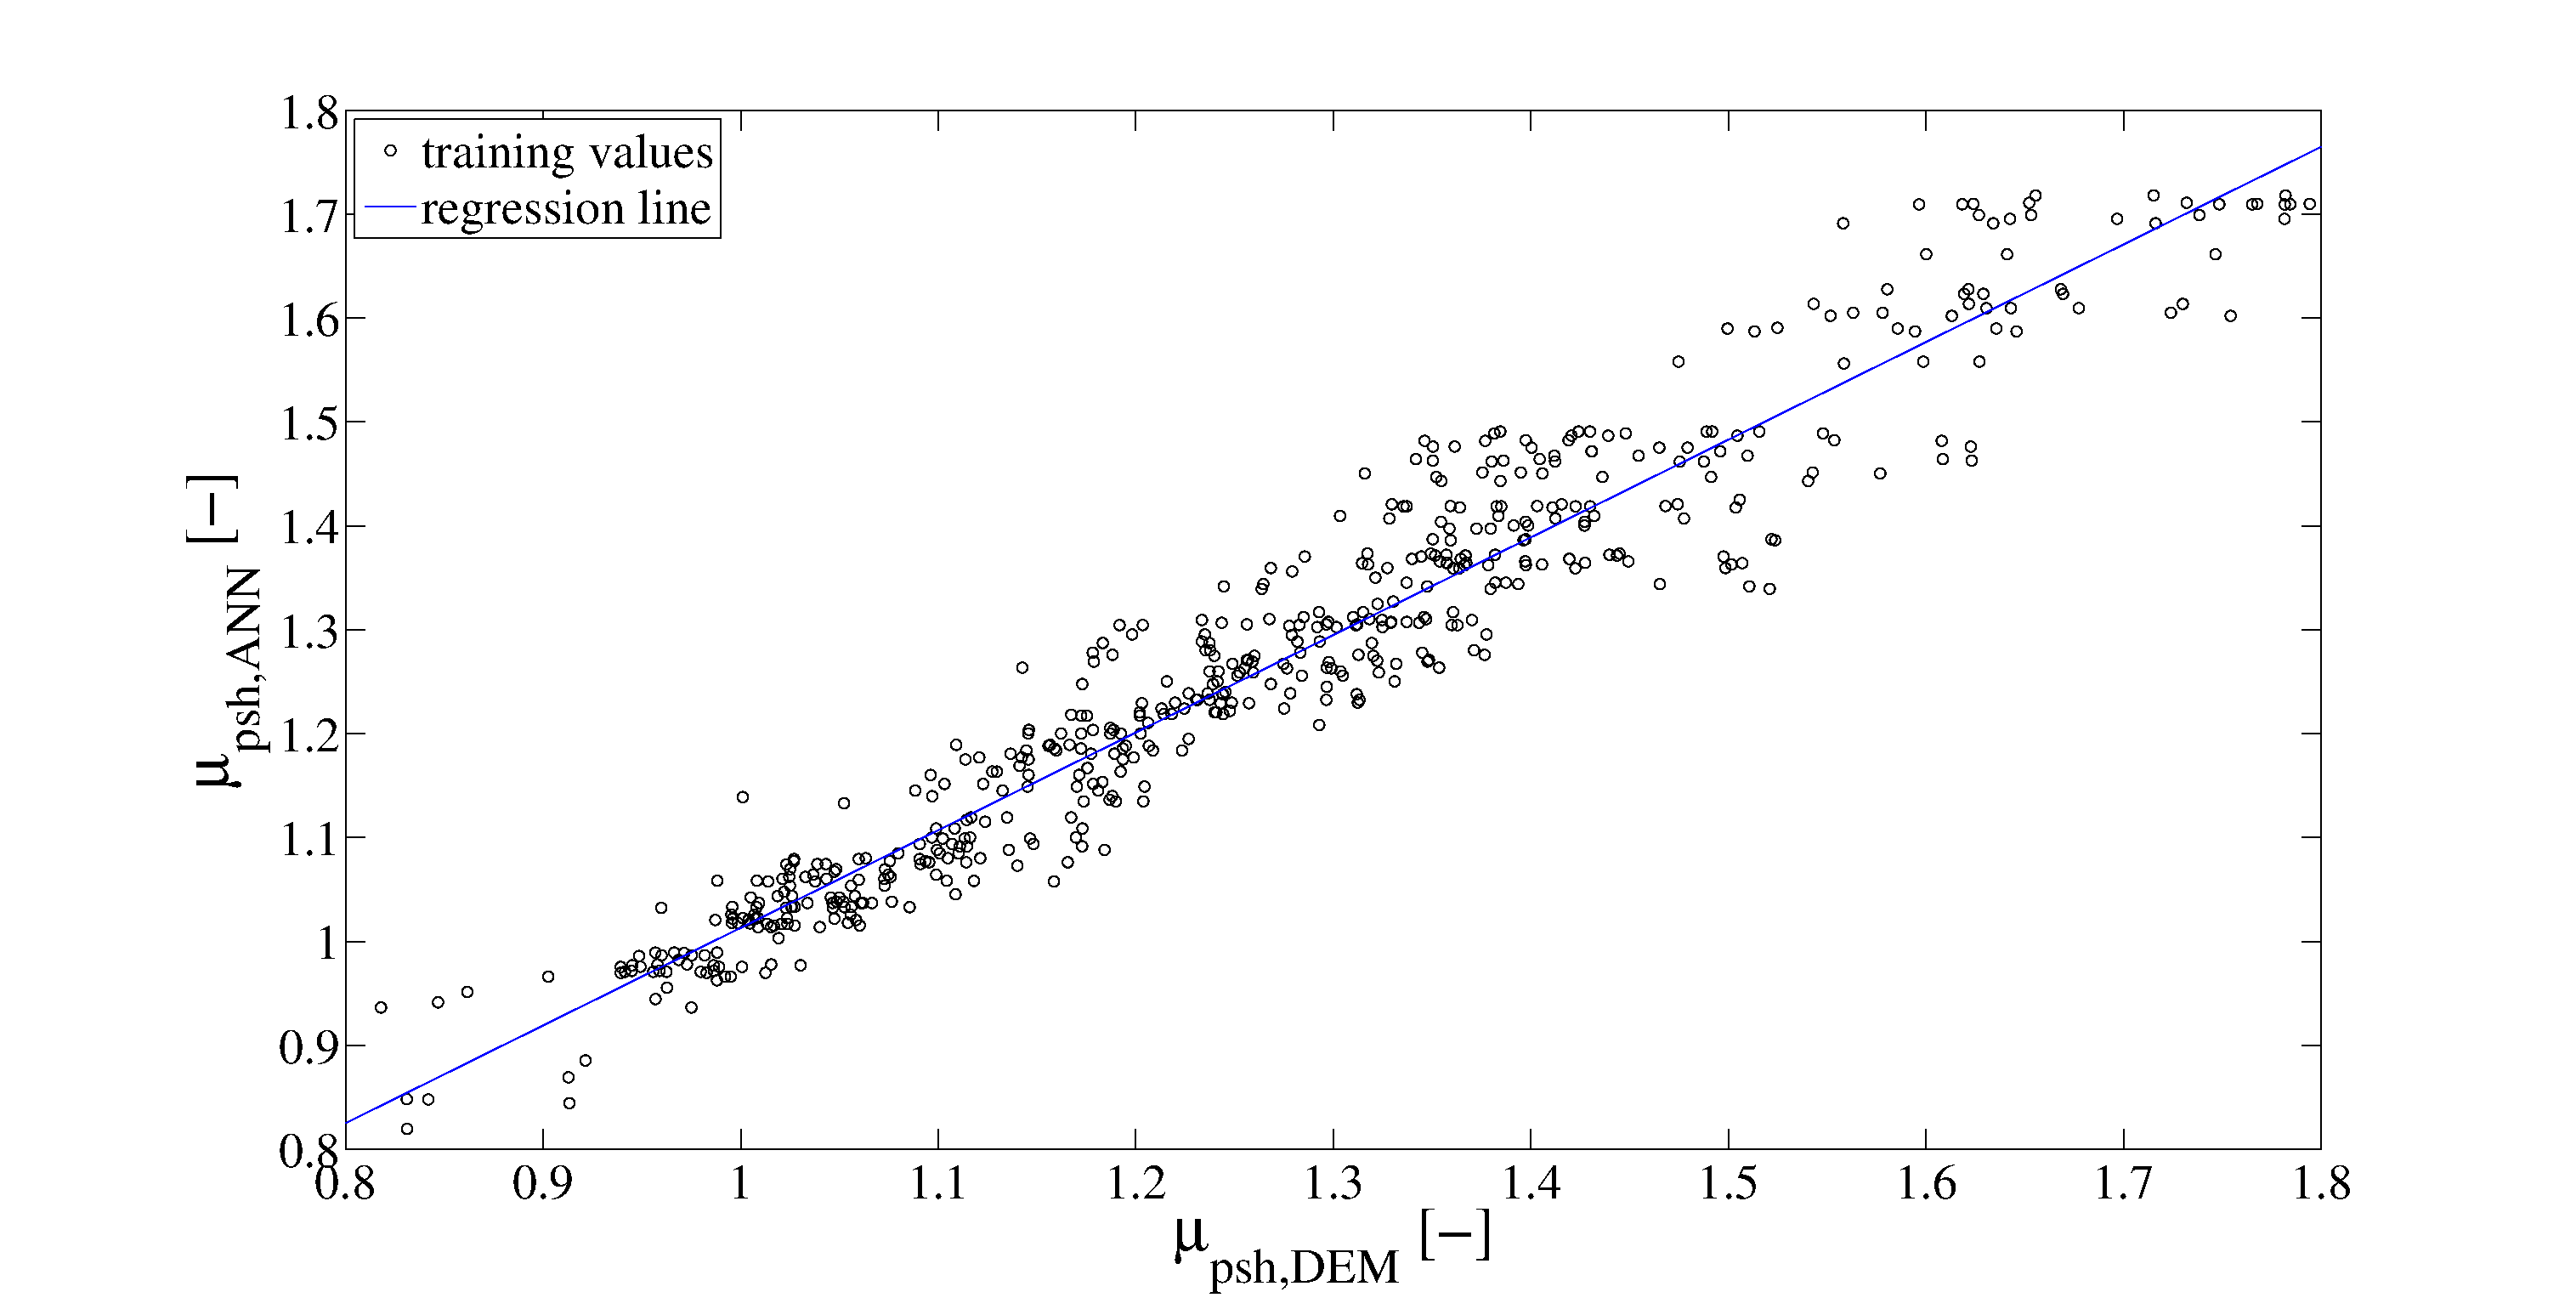
\includegraphics[width=.80\columnwidth]{images/022regression.eps}
% %[width=.48\textwidth]
% \caption[Comparison between prediction of the trained ANN and full DEM
% simulation]{Comparison between prediction of the trained Artificial Neural
% Network (\acs{ANN}) and 546 
% \wrong{write down all the simulations performed at the end.}
% full DEM simulations of the coefficient of pre-shear
% (\acs{mupsh}).}
% \label{fig:022regression} 
% \end{figure}

We checked \acs{r2}, \textit{mean absolute error}, 
\begin{equation}
MAE = \frac{\sum _{i=1}^{n} (x_{i}-\widehat{x}_{i})}{n}
\label{eq:meanAbsoluteError}
\end{equation}
\textit{mean squared error},
\begin{equation}
MSE = \frac{\sum _{i=1}^{n} (x_{i}-\widehat{x}_{i})^{2}}{n}
\label{eq:meanSquareError}
\end{equation}
and \textit{root mean squared error},
\begin{equation}
RMSE = \sqrt{\frac{\sum _{i=1}^{n} (x_{i}-\widehat{x}_{i})^{2}}{n}} ,
\label{eq:rootMeanSquareError}
\end{equation}
for the \textit{Bayesian linear
regression}, the \textit{Gaussian nonlinear
regression}, and the
\textit{\acs{ANN} regression} to establish the most effective method.
All were trained with the same training set. 
For instance, a comparison of the \acs{r2} for the \acs{mupsh} can be see in 
Fig. \ref{fig:143sctregressions}.
In Fig. \ref{fig:144aorregressions} a similar comparison for the \acs{AoR} can
be found.\\
In fact, the check was performed for each method by comparing the
\acs{DEM} bulk values of the test set against the bulk values predicted by each method from the 
corresponding \acs{DEM} input values of the test set. \\
Table \ref{tab:15regressionvalues} shows a quantitative comparison between the
three methods for the \acs{mupsh}. 
\begin{table}[htbp]
  \centering

    \begin{tabular}{lccc}
    \hline
          & Bayesian & Gaussian & ANN \\
          \hline
    Coefficient of determination (\acs{r2}) & 0.860  & 0.843 & 0.959 \\
    Root mean squared error & 0.057 & 0.061 & 0.031 \\
    Mean absolute error & 0.042 & 0.038 & 0.025 \\
    Mean squared error & 0.003 & 0.004 & 0.001 \\
    \hline
    \end{tabular}%
      \caption{Regression methods quantitative comparison.}
  \label{tab:15regressionvalues}%
\end{table}%
%************************************************

\section{Parameter Identification}
\label{sec:parameteridentification}

Since \acs{mupsh}, \acs{mush} and \acs{rhob} belonged to the shear-cell
simulations, their \acs{ANNs} were handled together: we had one cluster with three 
\acs{ANNs} for the shear cell and one with only one \acs{ANN} for the \acs{AoR}.
We could then proceed in identifying valid input parameters.

\subsection{Computational Condiderations}
\label{subsec:computationalcondiderations}

\citet{RefWorks:116, RefWorks:160} suggested using a Design of Experiments
(\acs{DoE}) method to determine the parameter combinations to be simulated.
They stated that this approach allows optimization of computation time
with an acceptable loss of precision.
The speed of the trained \acs{ANNs} enabled us to follow a different approach to
maximizing the precision of the characterization.\\

\begin{table}[h]
\centering
\begin{tabular}{lcccc}
\hline
 &  \ac{mus} & \ac{mur} & \ac{CoR} & \ac{rhop}  \\
  &	$[-]$  & $[-]$   & $[-]$   & $[kg/m3]$ \\
          \hline
    range & $[0.1 \ldots 1.0]$ & $[0.1 \ldots 1.0]$ & $[0.5 \ldots 0.9]$ &
    $[2000 \ldots 3500]$     \\
    \# rnd & 100   & 100   & 25    & 25    \\

\hline
\end{tabular}
\caption[DEM random input values]{DEM random input values. Within each range \#
random values are chosen.}
\label{tab:12DEMRandominputvalues}
\end{table}

\subsection{Decisional Limits}
\label{subsec:decisionallimits}

We created random values
in the range and numbers defined in Table \ref{tab:12DEMRandominputvalues}
according to a standard uniform distribution.
The total number of combinations of these random values was 6,250,000.
These combinations were then fed to and processed by the selected
\acs{ANNs}, and thus three bulk values for the shear
cell and one for the \acs{AoR} were obtained.
The \acs{ANN} evaluation was significantly faster than the \acs{DEM} simulations. The
individuation of the numerical bulk behaviours for all the \acs{DEM} combinations
did not take more than a few seconds on a single core.\\
\begin{figure}[!htb] 
\centering 
\includegraphics[width=.96\textwidth]{images/019methodology} 
\caption[Method]{Method. In the training phase (dashed lines)
$DEM$ simulations are performed
with random initial input parameters.
The behaviours obtained are used to train the
Artificial Neural Networks ($ANNs$) in a loop that continues until the
difference between the outputs of each $ANN$ and its simulations is below the
limit ($\Delta$).
In the parameters identification phase (solid
lines) we identify valid input parameters by comparing (\textbf{=}) $ANNs$ and
experimental behaviours.}
\label{fig:019methodology} 
\end{figure}
As can be seen in Fig. \ref{fig:019methodology}, in the parameters
identification phase (solid lines) we identify valid input parameters by comparing (\textbf{=}) \acs{ANNs} and
experimental behaviours.\\
We obtained for each of the twelve load conditions of the \acs{SCT} three bulk
values (\acs{mupsh}, \acs{mush} and \acs{rhob}).
The fourth bulk value was the result of two angle of repose (\acs{AoR}) tests that
recreated the repose angle observed in a pile of the
real material. 
Subsequently, we compared the \acs{ANN} and experimental bulk behaviours for the
twelve shear-cell load conditions.
If in a DEM-parameter combination all the three bulk values differed by less 
than 5\% from those of the corresponding experiments, i.e.:
%************************************************
 \begin{equation}
 \begin{cases}
\text{if } & \lvert{1-\frac{\mu_{psh,num}}{\mu_{psh,exp}}}\rvert < 5\%  ,\\
\text{and if } & \lvert{1-\frac{\mu_{sh,num}}{\mu_{sh,exp}}}\rvert < 5\% , \\ 
\text{and if } & \lvert{1-\frac{\rho_{p,num}}{\rho_{p,exp}}}\rvert < 5\% ,\\ 
\end{cases}
 \label{eq:check2}
\end{equation}

the combination was marked. The marked combinations were processed by the
\acs{AoR} \acs{ANN}, and then compared with the experiment.
Were considered valid those that differed by less than $5\%$ also in this
comparison (Eq. \ref{eq:checkaor}):
%************************************************
\begin{equation}
\text{if} ~~~~~~ \lvert{1-\frac{AoR_{num}}{AoR_{exp}}}\rvert < 5\% .
\label{eq:checkaor}
\end{equation}
%************************************************

\subsection{Reliability Considerations}
\label{subsec:reliabilityconsiderations}

We tested the marked combinations
by modifying the experimental bulk values of the shear cell to further prove
the validity of the system.
We artificially decreased or increased the shear force, and thus \acs{mupsh} and
\acs{mush}, by a product coefficient ($P$), e.g. Eq. \ref{eq:pcoeff}:
%************************************************
\begin{equation}
\label{eq:pcoeff}
\mu_{psh, new} = \mu_{psh, old} \cdot P .
\end{equation}
%************************************************

\subsection{Value representation}
\label{subsec:valuerepresentation}

\begin{itemize}
  \item{parameter space plot;}
  \item{box plot;}
  \item{density plot.}
\end{itemize}

\subsubsection{Parameter space plot}
\label{subsubsec:parameterspaceplot}

An example of a parameter space plot can be seen
in Fig. \ref{fig:041radarpirker1schulze1068}.
On the axes we can see:
\begin{itemize}
  \item{the \acl{CoR} (\acs{CoR}),}
  \item{the \acl{mus} (\acs{mus}),}
  \item{the \acl{mur} (\acs{mur}),}  
  \item{the \acl{rhob} (\acs{rhob}).}
\end{itemize}
Further, are shown:
\begin{itemize}
  \item{the minimum input values amongst the millions possible combinations,
  with a blue straight line;}
  \item{the minimum values amongst the valid, or marked combinations, with a
  green straight line;}
  \item{the mean values amongst the valid, or marked combinations, with an
  orange dotted line;}
  \item{the negative standard deviations from the mean values amongst the valid,
  or marked combinations, with a red straight line;}
  \item{the positive standard deviations from the mean values amongst the valid,
  or marked combinations, with a red straight line;}  
  \item{the maximum values amongst the valid, or marked combinations, with a
  green straight line;}
  \item{the maximum input values amongst the millions possible combinations,
  with a blue straight line.}  
\end{itemize}

The shaded area indicates valid parameter combinations, and dark shaded
values indicate the confidence range

\begin{figure}[htbp]
	\centering

    \subfloat[Parameter space plot, \acs{SCT}, $\sigma_n=1068$ Pa, P=0.8.]{
	  \includegraphics[width=.5\columnwidth]{images/150ParamSpaceSCT1068p08sinterfine}
	  \label{fig:150ParamSpaceSCT1068p08sinterfine}  }
	 
    \subfloat[Parameter space plot, \acs{SCT}, $\sigma_n=1068$ Pa, P=1.0.]{
	  \includegraphics[width=.5\columnwidth]{images/041radarpirker1schulze1068}
	  \label{fig:041radarpirker1schulze1068}  } 
	  
    \subfloat[Parameter space plot, \acs{SCT}, $\sigma_n=1068$ Pa, P=1.2.]{
	  \includegraphics[width=.5\columnwidth]{images/151ParamSpaceSCT1068p12sinterfine}
	  \label{fig:151ParamSpaceSCT1068p12sinterfine}  } 	  
	  

 % \hfill\null
  \caption[SCT parameter space plots 1]{SCT parameter space
  plots for sinter fine, $\sigma_n=1068$ Pa.}
  \label{fig:149paramspaceplotsct1068}
\end{figure}

% \begin{figure}%[!h] 
% \centering 
% 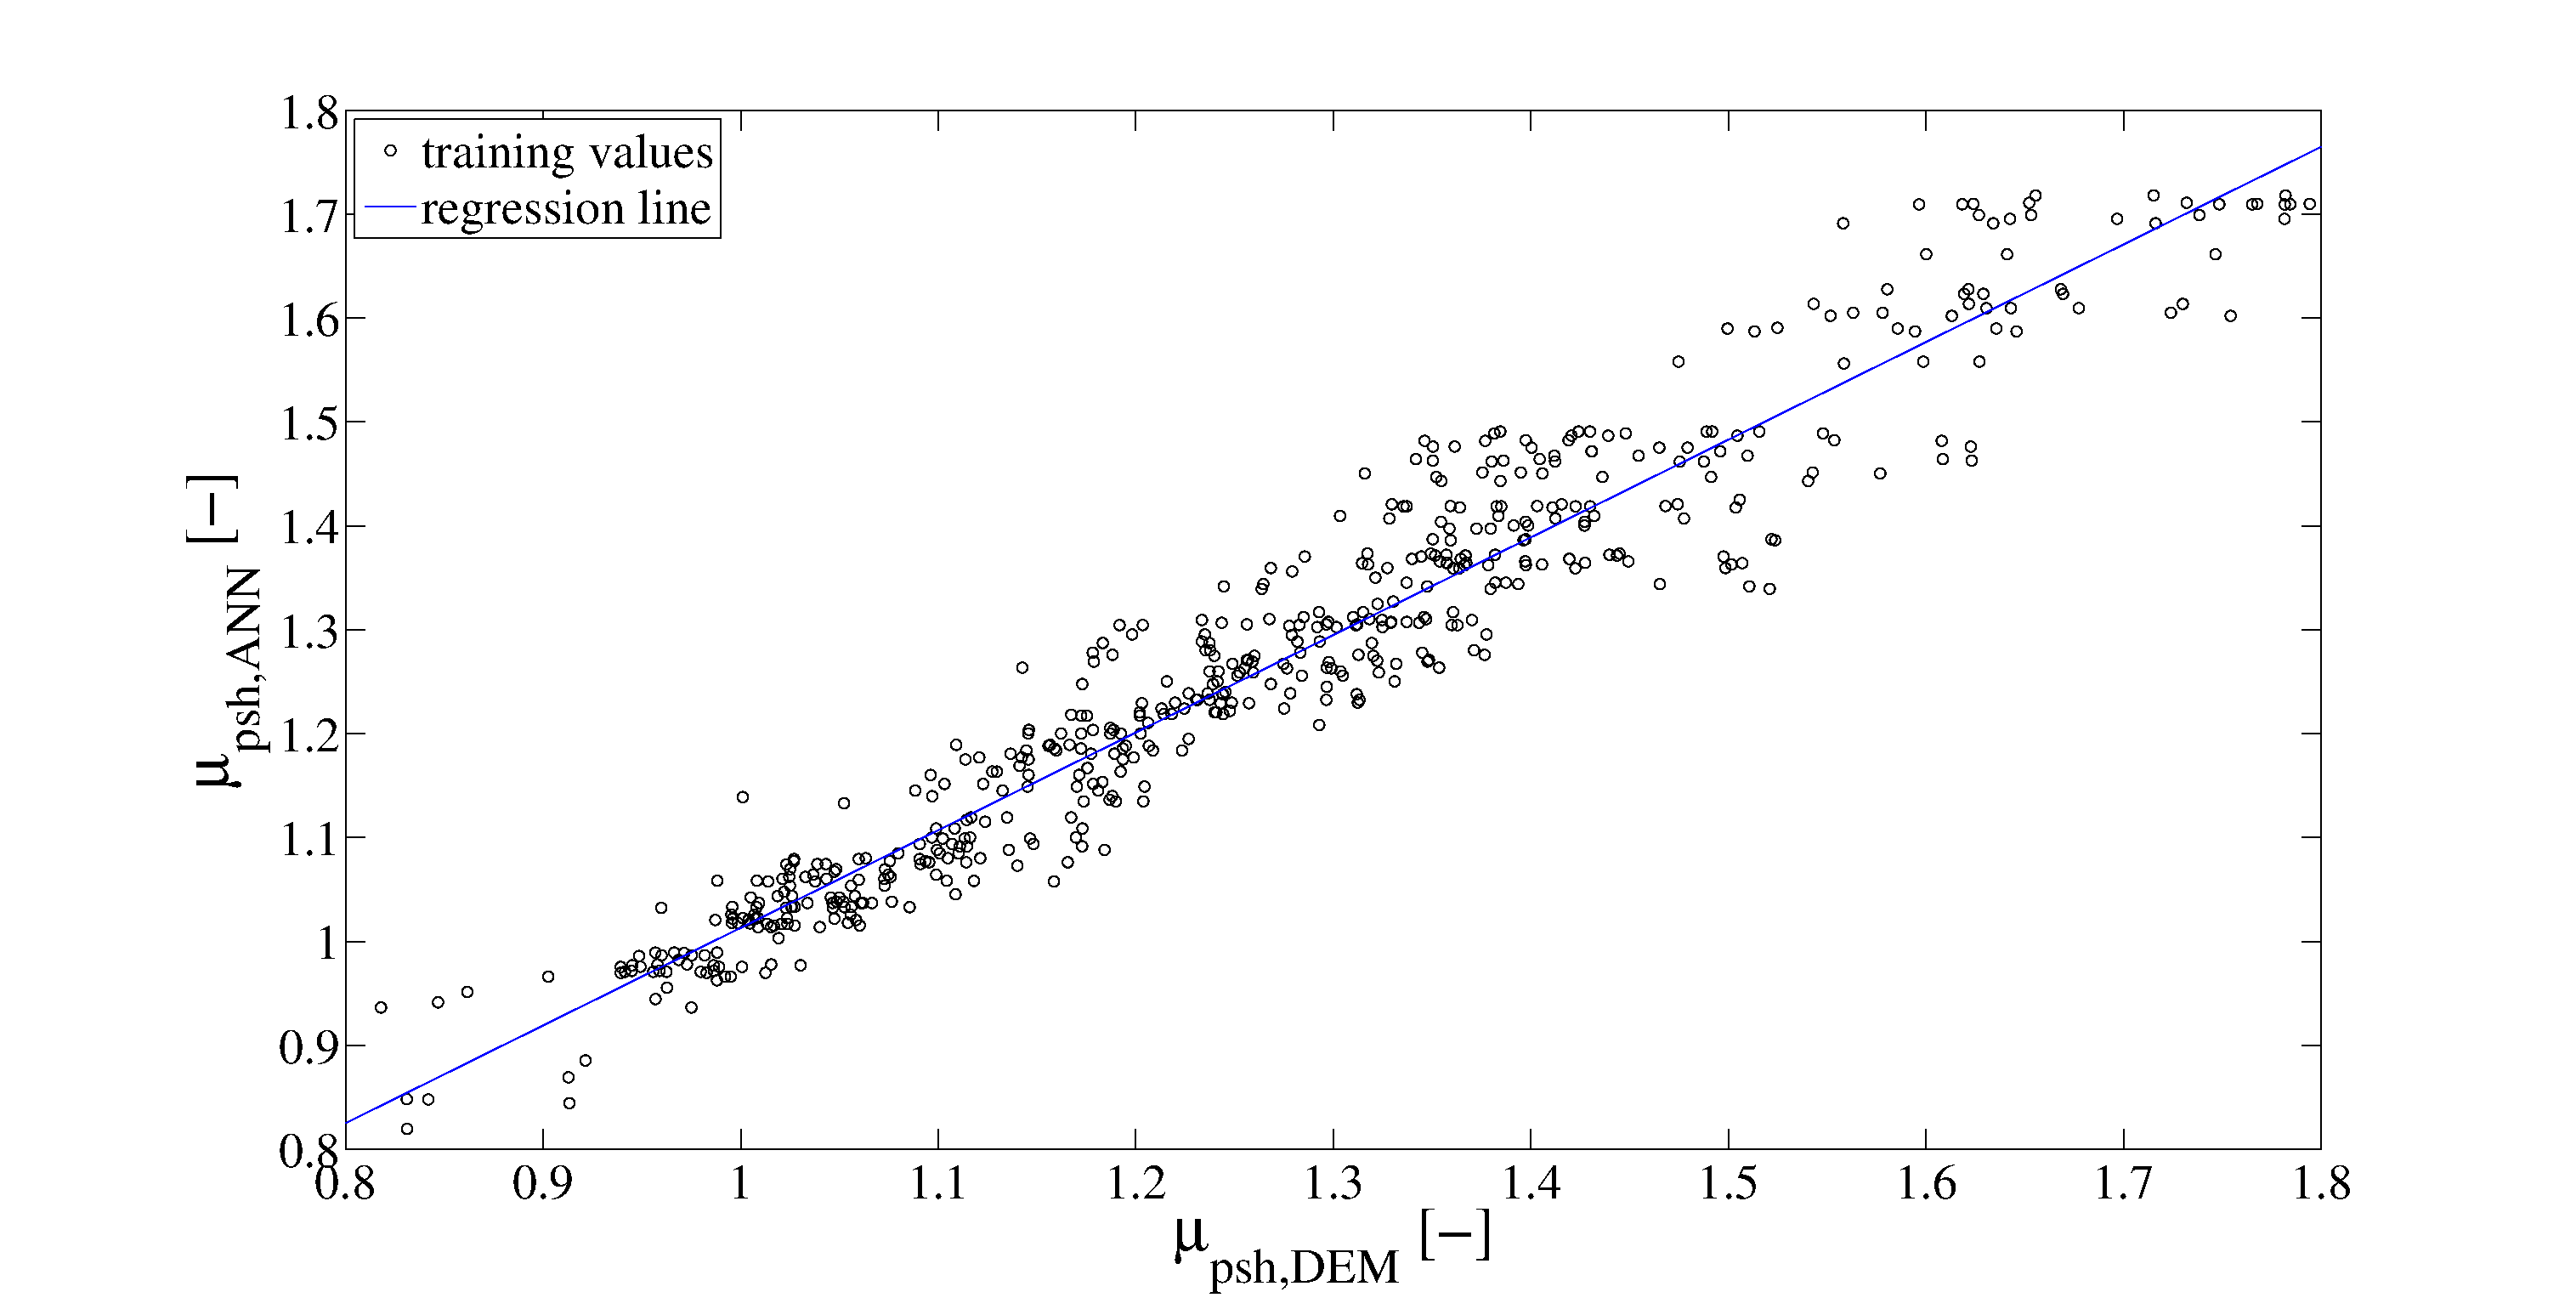
\includegraphics[width=.80\columnwidth]{images/022regression.eps}
% %[width=.48\textwidth]
% \caption[Comparison between prediction of the trained ANN and full DEM
% simulation]{Comparison between prediction of the trained Artificial Neural
% Network (\acs{ANN}) and 546 
% \wrong{write down all the simulations performed at the end.}
% full DEM simulations of the coefficient of pre-shear
% (\acs{mupsh}).}
% \label{fig:022regression} 
% \end{figure}


\subsubsection{Box plot}
\label{subsubsec:boxplot}
  
An example of a box plot can be seen
in Fig. \ref{fig:145BoxSCT1068p08sinterfine}.
\citet{RefWorks:207} defines a box plot a graphical representation of
collections of numerical data by means of their quartiles.
These are three points, which divide the data in four groups that are equals and
contain a quarter of the data each.\\
In a box plot the values between the first quartile (25\%) and the third
quartile (75\%) are included in a blue box.
Further, so called \textit{baffles} or \textit{whishers} are lines, which are
extended as far as the minimum and maximum values.
Finally, the median is represented as a red straight line.

\begin{figure}[htbp]
	\centering

    \subfloat[Box plot, \acs{SCT}, $\sigma_n=1068$ Pa, P=0.8.]{
	  \includegraphics[width=.75\columnwidth]{images/145BoxSCT1068p08sinterfine}
	  \label{fig:145BoxSCT1068p08sinterfine}  }
	 
    \subfloat[Box plot, \acs{SCT}, $\sigma_n=1068$ Pa, P=1.0.]{
	  \includegraphics[width=.75\columnwidth]{images/148BoxSCT1068p10sinterfine}
	  \label{fig:147BoxSCT1068p10sinterfine}  } 
	  
    \subfloat[Box plot, \acs{SCT}, $\sigma_n=1068$ Pa, P=1.2.]{
	  \includegraphics[width=.75\columnwidth]{images/147BoxSCT1068p12sinterfine}
	  \label{fig:148BoxSCT1068p12sinterfine}  } 	  
	  

 % \hfill\null
  \caption[SCT box plots 1]{SCT box
  plots for sinter fine, $\sigma_n=1068$ Pa.}
  \label{fig:146boxplotsct1068}
\end{figure}

% \begin{figure}%[!h] 
% \centering 
% 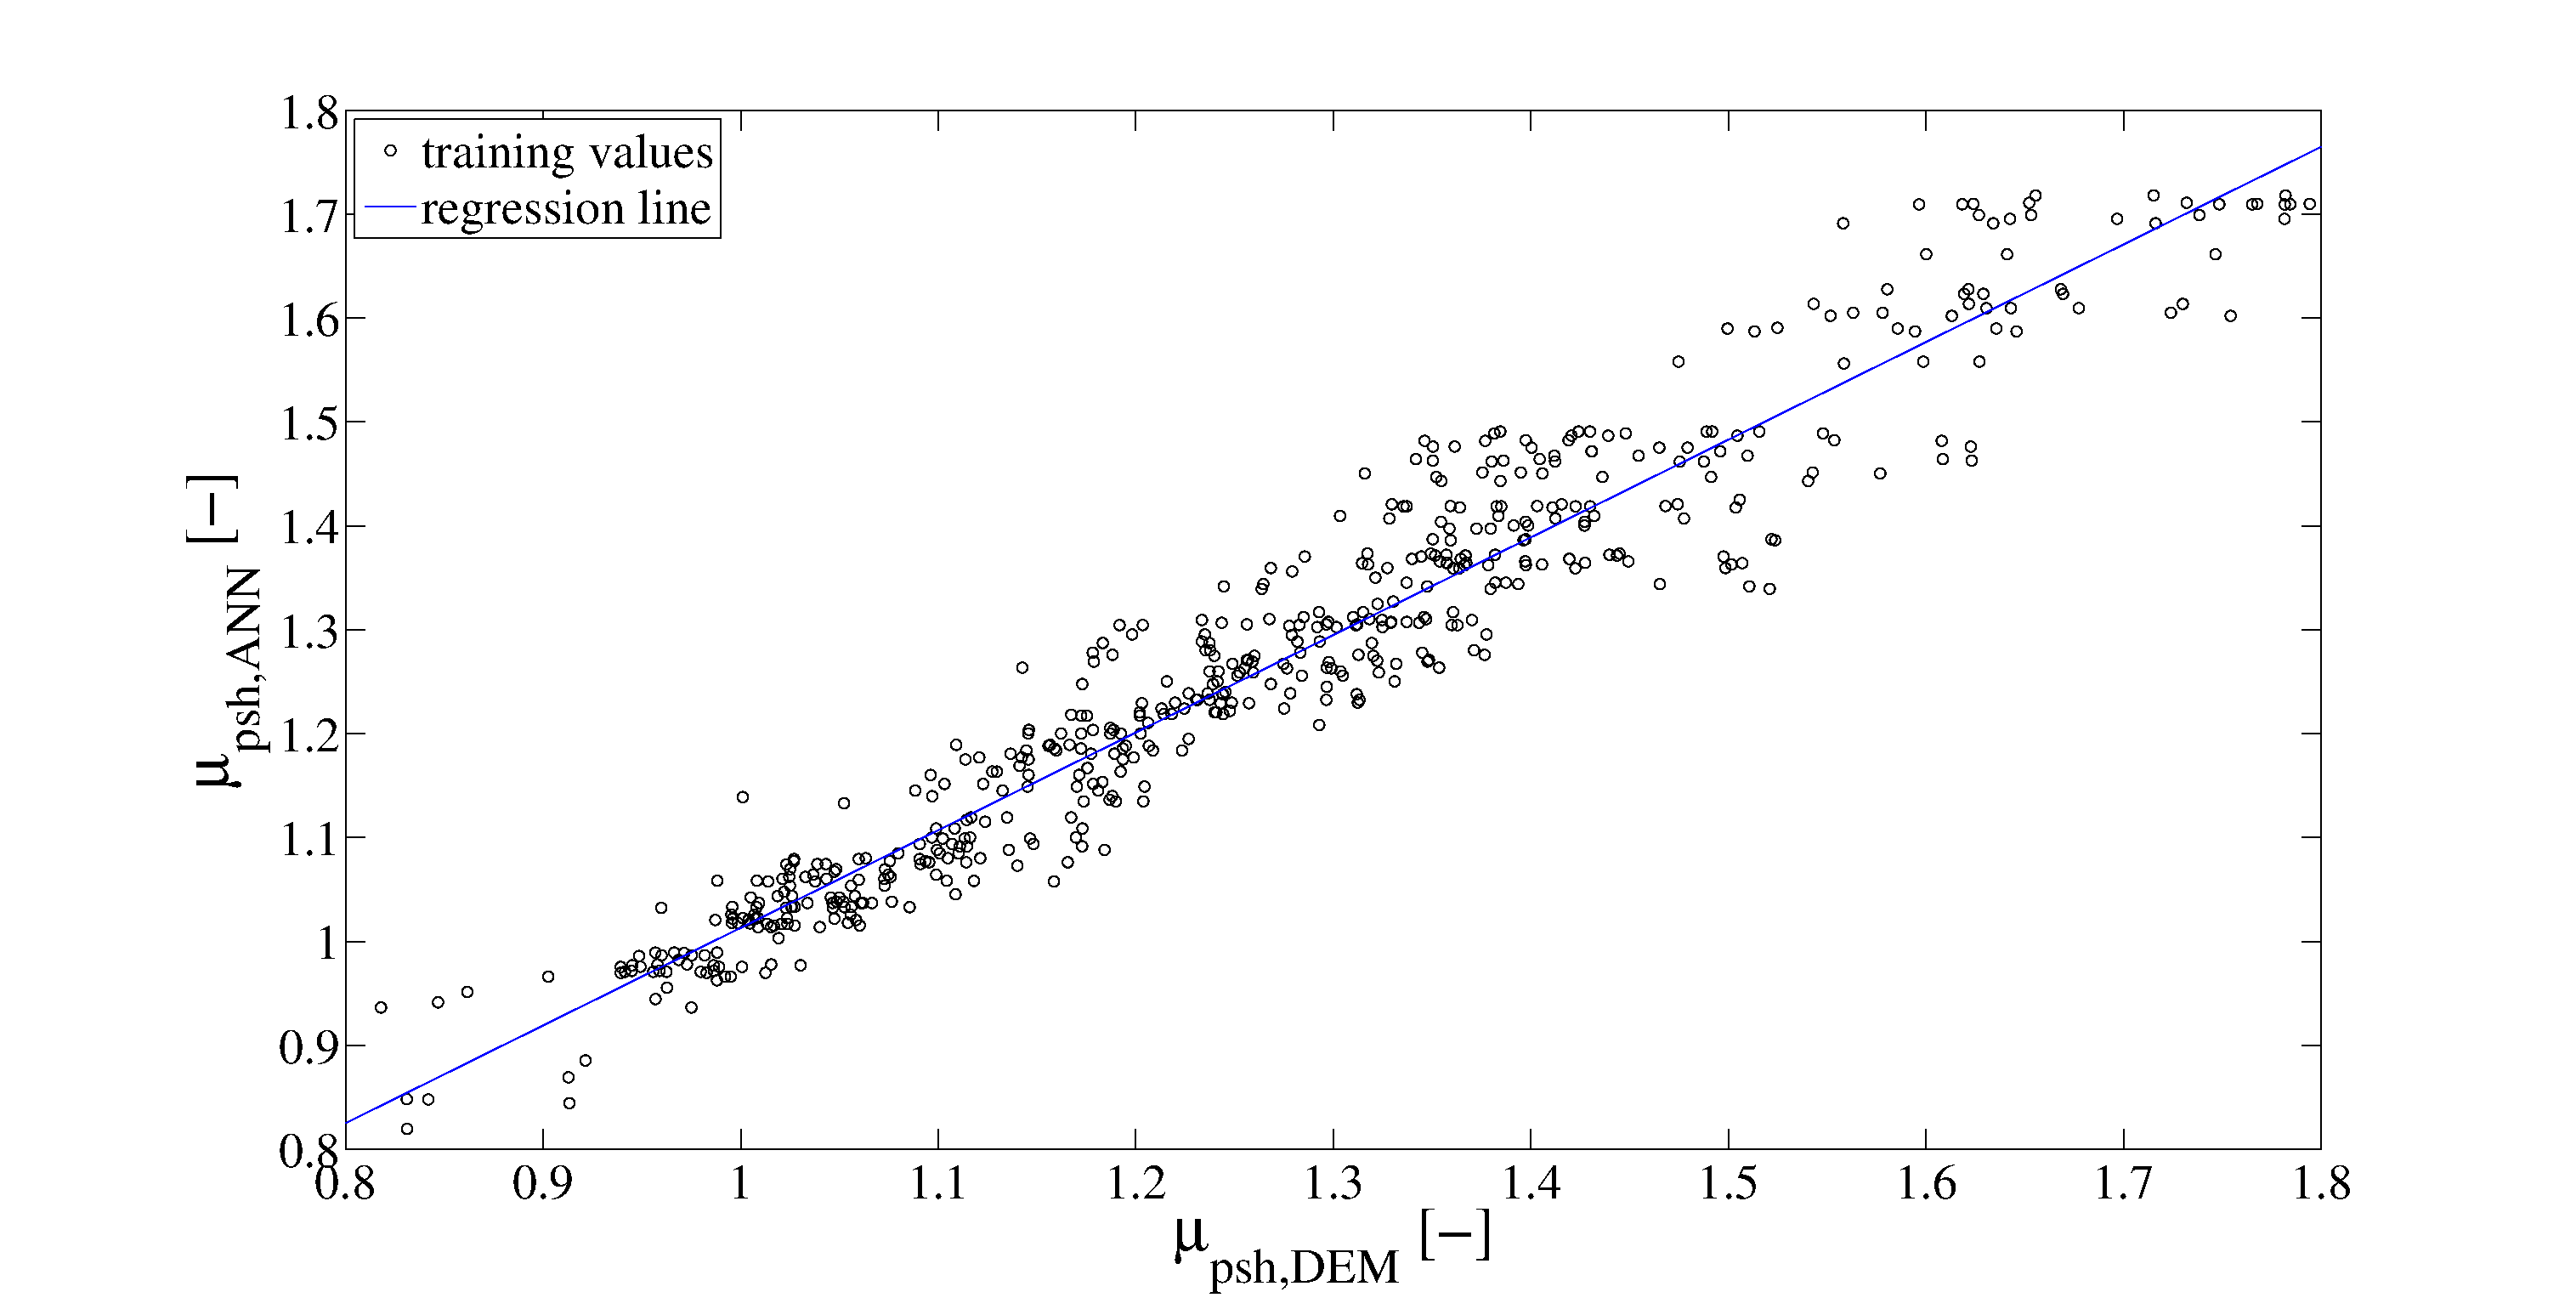
\includegraphics[width=.80\columnwidth]{images/022regression.eps}
% %[width=.48\textwidth]
% \caption[Comparison between prediction of the trained ANN and full DEM
% simulation]{Comparison between prediction of the trained Artificial Neural
% Network (\acs{ANN}) and 546 
% \wrong{write down all the simulations performed at the end.}
% full DEM simulations of the coefficient of pre-shear
% (\acs{mupsh}).}
% \label{fig:022regression} 
% \end{figure}

\subsubsection{Density plot}
\label{subsubsec:densityplot}

Further, we observed that various \acs{DEM} parameter
combinations could reproduce the experimental behaviour, and thus evaluated
their mutual dependencies.
This is shown more clearly in a density plot (e.g., Fig. 
\ref{fig:150ParamSpaceSCT1068p08sinterfine}) 
of the particles' coefficient of restitution (\acs{CoR}) in relation to
the coefficients of sliding friction (\acs{mus}) and rolling friction (\acs{mur}); 
in the white area, no valid sets of simulation parameters could be found.
In each cell the valid sets are grouped according to the 4 different COR
ranges.
Each cell is coloured according to the group with the most members.

\begin{figure}[htbp]
	\centering

    \subfloat[Density plot, \acs{SCT}, $\sigma_n=1068$ Pa, P=0.8.]{
	  \includegraphics[width=.75\columnwidth]{images/152TileSCT1068p08sinterfine}
	  \label{fig:152TileSCT1068p08sinterfine}  }
	 
    \subfloat[Density plot, \acs{SCT}, $\sigma_n=1068$ Pa, P=1.0.]{
	  \includegraphics[width=.75\columnwidth]{images/153TileSCT1068p10sinterfine}
	  \label{fig:153TileSCT1068p10sinterfine}  } 
	  
    \subfloat[Density plot, \acs{SCT}, $\sigma_n=1068$ Pa, P=1.2.]{
	  \includegraphics[width=.75\columnwidth]{images/154TileSCT1068p12sinterfine}
	  \label{fig:154TileSCT1068p12sinterfine}  } 	  
	  

 % \hfill\null
  \caption[SCT Density plots 1]{SCT Density
  plots for sinter fine, $\sigma_n=1068$ Pa.}
  \label{fig:155tileplotsct1068sinterfine}
\end{figure}

% \begin{figure}%[!h] 
% \centering 
% 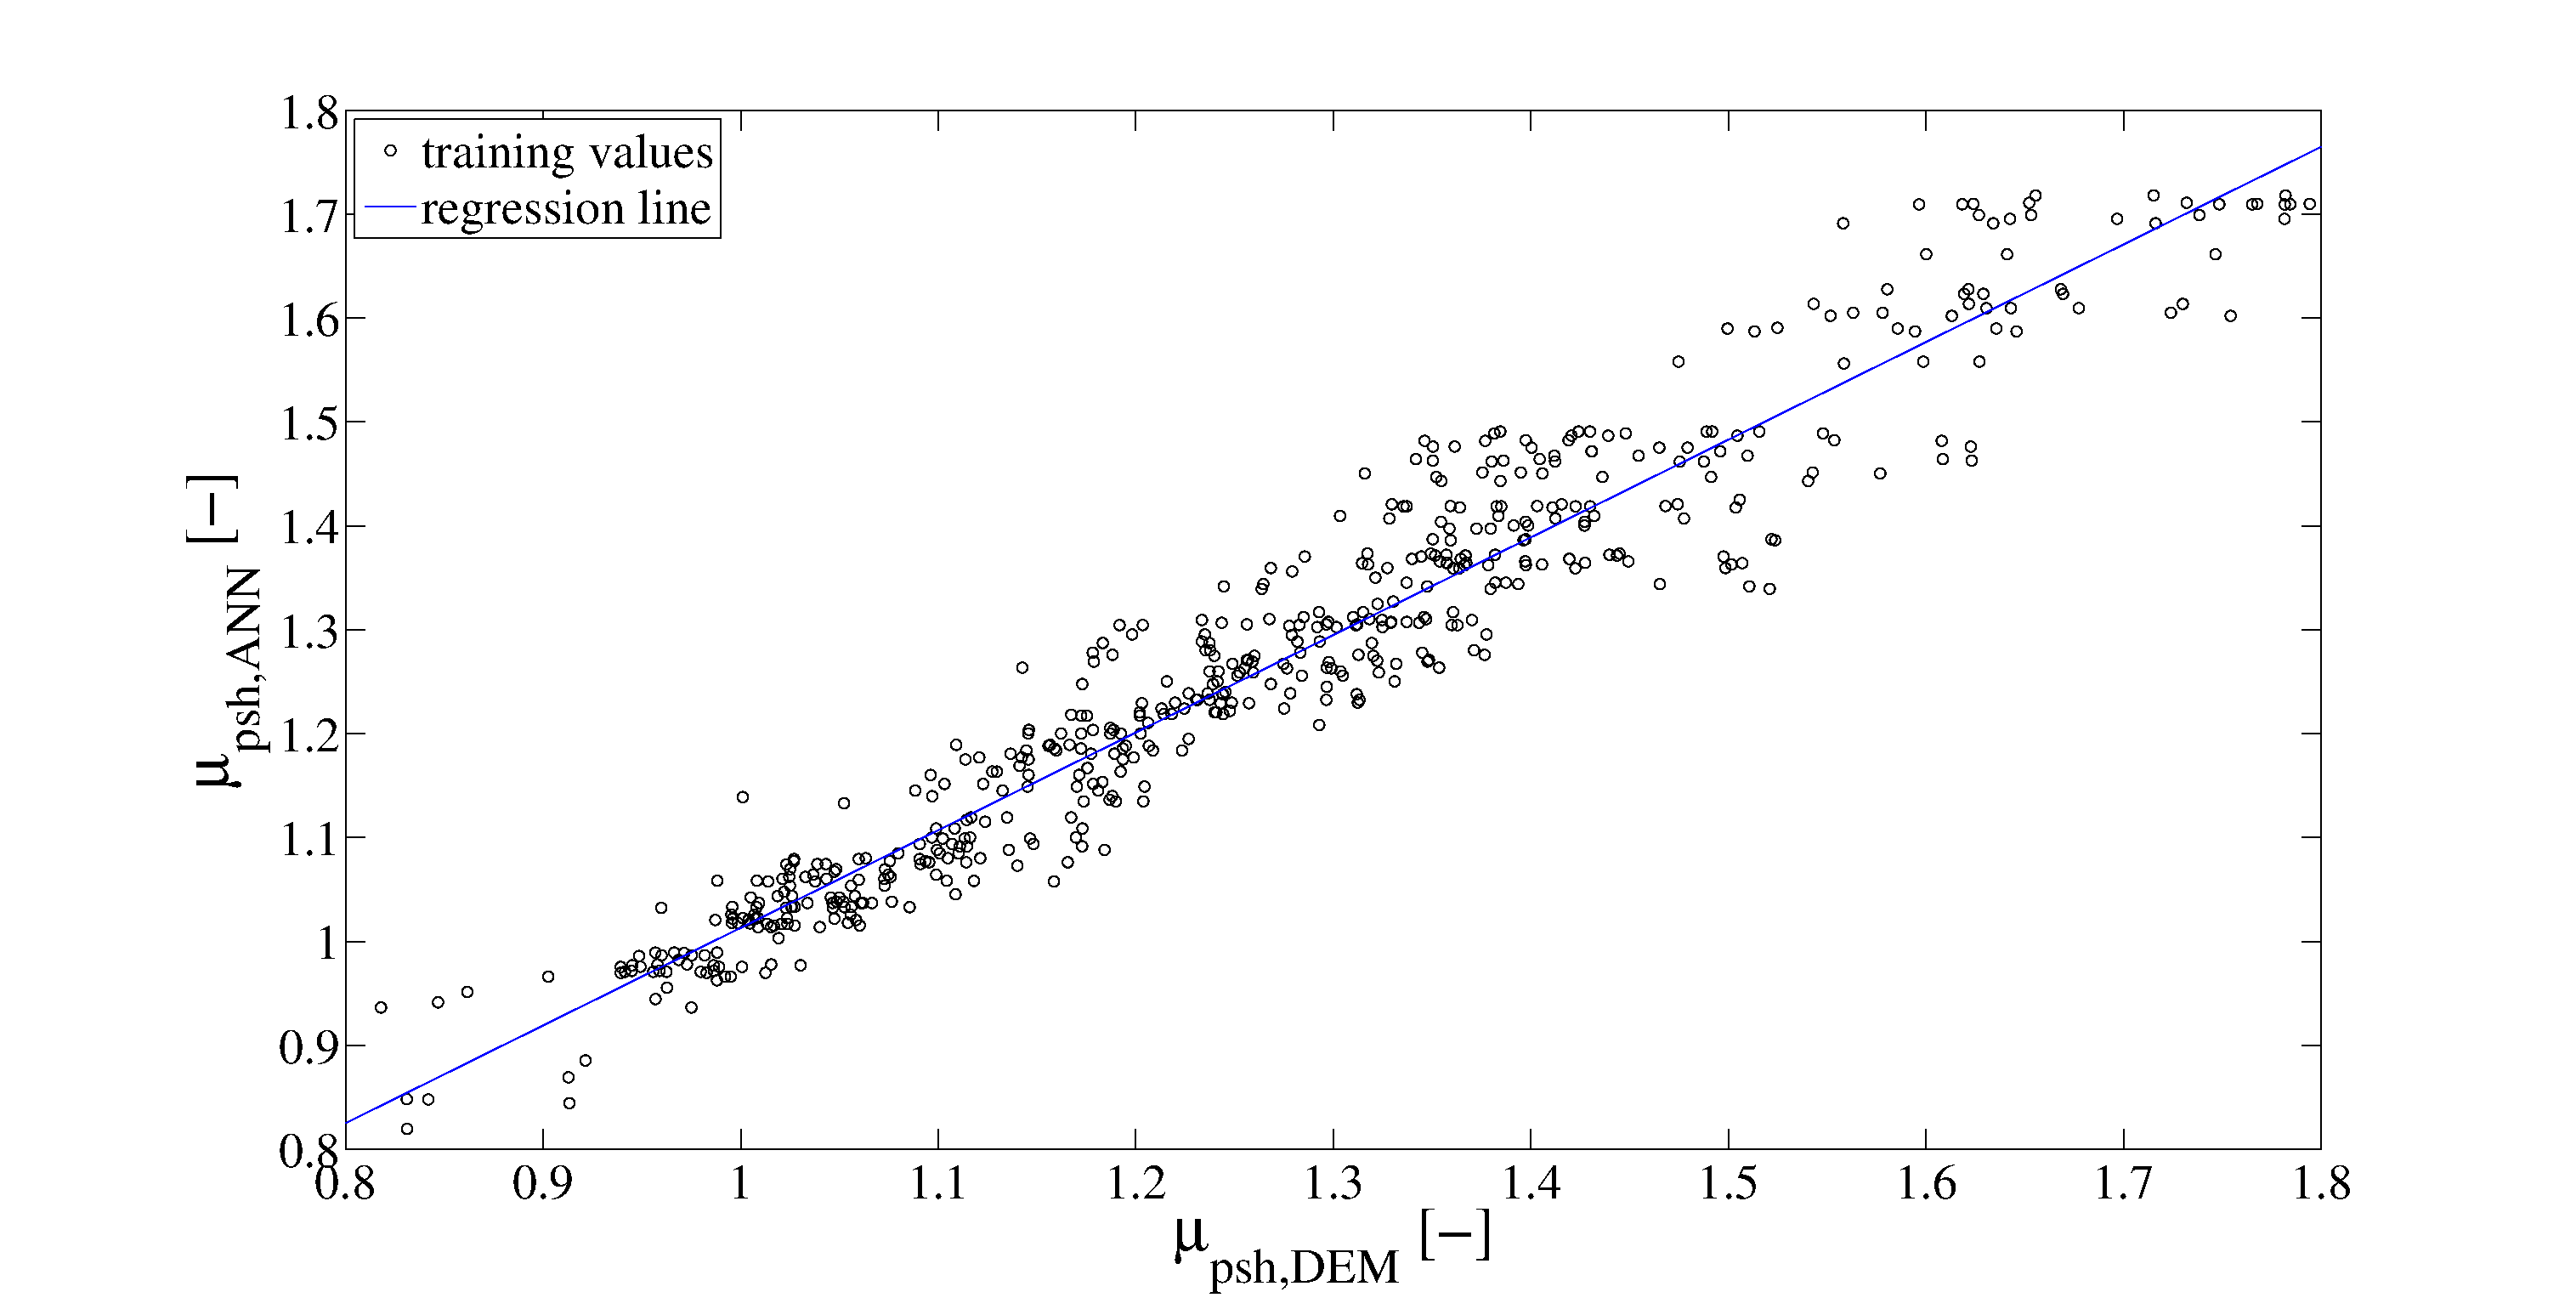
\includegraphics[width=.80\columnwidth]{images/022regression.eps}
% %[width=.48\textwidth]
% \caption[Comparison between prediction of the trained ANN and full DEM
% simulation]{Comparison between prediction of the trained Artificial Neural
% Network (\acs{ANN}) and 546 
% \wrong{write down all the simulations performed at the end.}
% full DEM simulations of the coefficient of pre-shear
% (\acs{mupsh}).}
% \label{fig:022regression} 
% \end{figure}

%************************************************
%************************************************

\subsection{SCT parameter space plot for Sinter fine}
\label{subsec:sctparameterspacesinterfine}

\begin{figure}[htbp]
\centering 
%   \subfloat[Parameter space plot, \acs{SCT}, $\sigma_n=1068$ Pa, P=1.0.]{
% 	  \includegraphics[width=.35\columnwidth]{images/041radarpirker1schulze1068}
% 	  \label{fig:041radarpirker1schulze1068}
%   }
%   \\
    \subfloat[Parameter space plot, \acs{SCT}, $\sigma_n=10070$ Pa, P=0.8.]{
	  \includegraphics[width=.5\columnwidth]{images/026radarpirker08schulze10070}
	  \label{fig:026radarpirker08schulze10070}
  }
  \\
  \subfloat[Parameter space plot, \acs{SCT}, $\sigma_n=10070$ Pa, P=1.0.]{
	  \includegraphics[width=.5\columnwidth]{images/024radarpirker1schulze10070}
	  \label{fig:024radarpirker1schulze10070}
  }
  \\
    \subfloat[Parameter space plot, \acs{SCT}, $\sigma_n=10070$ Pa, P=1.2.]{
	  \includegraphics[width=.5\columnwidth]{images/028radarpirker12schulze10070}
	  \label{fig:028radarpirker12schulze10070}
  }
  \caption[SCT parameter space plots 2]{SCT parameter space
  plots, $\sigma_n=10070$ Pa. The valid parameters are plotted over four axes,
  accounting for average and standard deviation.}
  \label{fig:079sctparameterspaceplots}
\end{figure}

The comparison between numerical and experimental behaviours led to a first
series of marked combinations ($MC1$) for two load conditions of
the shear cell:
\begin{itemize}
  \item{$\acs{sigman} = 1,068$ Pa, P=1.0, as plotted in Fig.
  \ref{fig:041radarpirker1schulze1068},}
  \item{$\acs{sigman} = 10,070$ Pa, P=1.0, as plotted in Fig.
  \ref{fig:024radarpirker1schulze10070}.}
\end{itemize}
Note that the confidence interval is large, 
especially for the \acs{CoR}, which highlights its insignificant influence on the
characterization.
Both the \acs{rhop}  and the \acs{mus}, however, show a narrow confidence interval, 
which demonstrates their influence and the ability of this procedure to find
valid \acs{DEM} parameters.
These results agree with our examination of the ratio of the standard deviation
to the range, see Table \ref{tab:13DEMvalidvalues}.

\subsection{SCT box plot for Sinter fine}
\label{subsec:sctboxsinterfine}

\begin{figure}[htbp]
\centering 
%   \subfloat[Parameter space plot, \acs{SCT}, $\sigma_n=1068$ Pa, P=1.0.]{
% 	  \includegraphics[width=.35\columnwidth]{images/041radarpirker1schulze1068}
% 	  \label{fig:041radarpirker1schulze1068}
%   }
%   \\157BoxSCT10070p08sinterfine.png
%158BoxSCT10070p12sinterfine.png
    \subfloat[Box plot, \acs{SCT}, $\sigma_n=10070$ Pa, P=0.8.]{
	  \includegraphics[width=.70\columnwidth]{images/157BoxSCT10070p08sinterfine}
	  \label{fig:157BoxSCT10070p08sinterfine}  }
  \\
    \subfloat[Box plot, \acs{SCT}, $\sigma_n=10070$ Pa, P=1.0.]{
	  \includegraphics[width=.70\columnwidth]{images/075sctboxplot}
	  \label{fig:075sctboxplot}  }
  \\
    \subfloat[Box plot, \acs{SCT}, $\sigma_n=10070$ Pa, P=1.2.]{
	  \includegraphics[width=.70\columnwidth]{images/158BoxSCT10070p12sinterfine}
	  \label{fig:158BoxSCT10070p12sinterfine}  }
  \\
  \caption[SCT box plots for sinter fine]{SCT box
  plots for sinter fine, $\sigma_n=10070$ Pa. The range of valid parameters is
  shown, together with the average and the 25 and 75 percentile.}
  \label{fig:156boxplotsct10070sinterfine}
\end{figure}

\subsection{SCT cloud space}
\label{subsec:sctcloudspace}

Multiple
combinations (250,407 or 4\% of the total) of \acs{mus} and \acs{mur} reproduced
the experimental behaviour with varying \acs{CoR}.
This underlines once more their correlation, as already stated by Wensrich and 
Katterfeld \cite{RefWorks:87}.

\begin{figure}[htbp]
\centering 
  \subfloat[Density plot, \acs{SCT}, $\sigma_n=10070$ Pa, P=0.8.]{
	  \includegraphics[width=.75\columnwidth]{images/159TileSCT10070p08sinterfine}
	  \label{fig:159TileSCT10070p08sinterfine}
  }
  \\
    \subfloat[Density plot, \acs{SCT}, $\sigma_n=10070$ Pa, P=1.0.]{
	  \includegraphics[width=.75\columnwidth]{images/160TileSCT10070p10sinterfine}
	  \label{fig:160TileSCT10070p10sinterfine}
  }
  \\
  \subfloat[Density plot, \acs{SCT}, $\sigma_n=10070$ Pa, P=1.2.]{
	  \includegraphics[width=.75\columnwidth]{images/161TileSCT10070p12sinterfine}
	  \label{fig:161TileSCT10070p12sinterfine}
  }
  \\
  \caption{Density plot comparison of SCT results.}
  \label{fig:080sctdensityplots}
\end{figure}

\subsection{Product coeffiecient effect}
\label{subsec:productcoeffiecienteffect}

To further demonstrate the validity of the procedure, we modified the product
coefficient. 
First, we set it to $P=0.8$, and we obtained another
series of marked combinations ($MC2$).
It could be seen in the parameter space plot in Fig.
\ref{fig:026radarpirker08schulze10070} that the confidence range is narrower
than for $P=1.0$, while in the density plot in Fig. 
\ref{fig:159TileSCT10070p08sinterfine} the area
appears larger, although slightly less densely populated. Finally, for $P=1.2$
and its marked combinations ($MC3$) the parameter space plot in Fig.
\ref{fig:028radarpirker12schulze10070} shows a largely different confidence
range, while the density plot in Fig. \ref{fig:161TileSCT10070p12sinterfine} 
shows a smaller area. As expected, the procedure was highly sensitive to
variations in the experimental data.
Our approach could therefore be used
for a wide range of bulk materials.\\

\subsection{AoR and merge results}
\label{subsec:aorandmergeresults}

We then processed the random combinations with the \acs{AoR} \acs{ANN}. In Fig.
\ref{fig:031radarpirker1aor} the parameter space plot for the same criteria as
before could be seen.
In accordance with theory (Wensrich and Katterfeld \cite{RefWorks:87}), in a simulation dominated
by rolling particles, the coefficient of rolling friction has the maximum
influence. \\
Finally, we extracted from the $MC1$ values the \acs{AoR} \acs{ANN} behaviour
and compared it with the experimental one.
As could be seen in the parameter space plot in Fig.
\ref{fig:033radarpirker1schulze10070aor}, the confidence interval is very small,
indicating that all the parameters but the \acs{CoR} played an important role, 
and demonstrating the reliability of these parameter
combinations in representing the bulk behaviour.
From the initial 6,250,000 combinations, only 3,884 were valid (0.0621
\%), see Table \ref{tab:13DEMvalidvalues}.
%************************************************
% \begin{table}[h]
\centering
\begin{tabular}{cccccc}
$\sigma_n$ [Pa] & $\tau$ [Pa] & $\mu_{psh}$ [-] & $\mu_{sh}$ [-] &
$\rho_b$ [kg/m3] & AOR $\circ$ \\
\hline
    1068  & 1059  & 0.9916 & 0.9916 & 1718  & 38.85 \\
    2069  & 1818  & 0.8787 & 0.8787 & 1759  & 38.85 \\
    10070 & 8232  & 0.8175 & 0.8175 & 1802  & 38.85 \\

\hline
\end{tabular}
\caption{Experimental values for sinter fine}
\label{tab:05sinterTableExperimental}
\end{table}
% \info{one table for each material? here or in the polydispersity chapter?}

\begin{table}[h]
\centering
\scalebox{0.7}{
\begin{tabular}{llccc}
\hline

          & type  & SCT & AOR   & SCT \& AOR \\
          \hline

    $\mu_s$ & mean  & 0.831 & 0.177 & 0.664 \\
    $[-]$   & std. dev. (SD) & 0.097 & 0.095 & 0.029 \\
          & range ($R$) & 0.9   & 0.9   & 0.9 \\
          & SD / R & 0.108 & 0.106 & 0.032 \\
          \hline
    $\mu_r$ & mean  & 0.692 & 0.830 & 0.916 \\
    $[-]$   & std. dev. (SD) & 0.215 & 0.193 & 0.042 \\
          & range ($R$) & 0.9   & 0.9   & 0.9 \\
          & SD / R & 0.239 & 0.214 & 0.046 \\
          \hline
              COR   & mean  & 0.708 & 0.590 & 0.590 \\
   $ [-]$   & std. dev. (SD) & 0.104 & 0.073 & 0.065 \\
          & range ($R$) & 0.4   & 0.4   & 0.4 \\
          & SD / R & 0.259 & 0.183 & 0.161 \\
          \hline
    $\rho_p$ & mean  & 2245.7 & 3192.8 & 2283.9 \\
    $[kg/m3]$ & std. dev. (SD) & 80.5  & 277.4 & 67.1 \\
          & range ($R$) & 1500  & 1500  & 1500 \\
          & SD / R & 0.054 & 0.185 & 0.045 \\
          \hline
    valid & number & 290203 & 816552 & 3884 \\
    combinations & [$\%$] & 4.64  & 13.06 & 0.06 \\
    

\hline
\end{tabular}}
\caption{DEM valid values.}
\label{tab:13DEMvalidvalues}
\end{table}


%************************************************


%081aorandmergeparameterspaceplots}
\begin{figure}[htbp]
\centering 
  \subfloat[Parameter space plot, $AoR_{exp} = 38.85 ^\circ$.]{
	  \includegraphics[width=.50\columnwidth]{images/031radarpirker1aor}
	  \label{fig:031radarpirker1aor}
  }
  \\
    \subfloat[Box plot, $AoR_{exp} = 38.85 ^\circ$.]{
	  \includegraphics[width=.60\columnwidth]{images/076aorboxplot}
	  \label{fig:076aorboxplot}
  }
  \\
    \subfloat[Density plot plot, $AoR_{exp} = 38.85
        ^\circ$.]{
	  \includegraphics[width=.60\columnwidth]{images/162TileAORsinterfine}
	  \label{fig:162TileAORsinterfine}  }
  \\
  \caption[AoR valid values plots]{\acs{AoR} valid values plots. The valid
  values for the \acs{AoR} sinter fine test are shown in three different plots.
  The results are clearly different from the \acs{SCT} test and the \acs{mur}
  is the most relevant parameter.}
  \label{fig:207aorparameterspaceplots}
\end{figure}
\begin{figure}[htbp]
\centering 
  \subfloat[Parameter space plot, $AoR_{exp} = 38.85 
        ^\circ$ \& \acs{SCT}: $\sigma_n=10070$ Pa.]{
	  \includegraphics[width=.50\columnwidth]{images/033radarpirker1schulze10070aor}
	  \label{fig:033radarpirker1schulze10070aor}
  }
  \\
    \subfloat[Box plot, $AoR_{exp} = 38.85
        ^\circ$ \& \acs{SCT}: $\sigma_n=10070$ Pa.]{
	  \includegraphics[width=.60\columnwidth]{images/078mergeboxplot}
	  \label{fig:078mergeboxplot}  }
  \\
  \subfloat[Density plot plot, $AoR_{exp} = 38.85 
        ^\circ$ \& \acs{SCT}: $\sigma_n=10070$ Pa.]{
	  \includegraphics[width=.60\columnwidth]{images/206TileMixsinterfine_33}
	  \label{fig:206TileMixsinterfine_33}
  }
  \\  
  \caption[Merge parameter space plots of the sinter fine]{Merge parameter space
  plots of the sinter fine. A limited number of parameters are valid for both
  tests. It is clear that the friction coefficients are the most relevant micro
  parameters and only a small range of their values can be used to successfully model the bulk behaviour of the
  sinter fine.}
  \label{fig:208mergeparameterspaceplots}
\end{figure}


%************************************************
%************************************************

\section{Influence of poly-dispersity}
\label{sec:polydispersity}
%************************************************

% \info{Some examples of the new images: relationship between the standard
% deviation of the radius and the shape of the tile plot.}
% 
% \improvement{table similar to \ref{tab:12DEMRandominputvalues} here}
% \wrong{separate all images into single with captions}
% \change{add box plots?}
% 
% Fig. \ref{fig:082ironore0315}\\
% \begin{figure}[!htb]
\centering
\includegraphics[width=.96\columnwidth]{images/082ironore0315}
\caption[Iron ore fine polidispersity evaluation]{Iron ore fine polidispersity evaluation.}
\label{fig:082ironore0315}
\end{figure}
% 
% Fig. \ref{fig:083ironore31510}\\
% \begin{figure}[!htb]
\centering
\includegraphics[width=.96\columnwidth]{images/083ironore31510}
\caption[Iron ore coarse polydispersity evaluation]{Iron ore coarse polydispersity
evaluation.}
\label{fig:083ironore31510}
\end{figure}
% 
% Fig. \ref{fig:084limestone0315}\\
% \begin{figure}[!htb]
\centering
\includegraphics[width=.96\columnwidth]{images/084limestone0315}
\caption[Limestone fine polidispersity evaluation]{Limestone fine polidispersity evaluation.}
\label{fig:084limestone0315}
\end{figure}
% 
% Fig. \ref{fig:085limestone31510}\\
% \begin{figure}[!htb]
\centering
\includegraphics[width=.96\columnwidth]{images/085limestone31510}
\caption[Limestone coarse polidispersity evaluation]{Limestone coarse polidispersity
evaluation.}
\label{fig:085limestone31510}
\end{figure}
% 
% Fig. \ref{fig:086sinter0315}\\
% \begin{figure}[!htb]
\centering
\includegraphics[width=.96\columnwidth]{images/086sinter0315}
\caption[Sinter fine polydispersity evaluation]{Sinter fine polydispersity evaluation.}
\label{fig:086sinter0315}
\end{figure}
% 
% Fig. \ref{fig:087sinter31510}\\
% \begin{figure}[!htb]
\centering
\includegraphics[width=.96\columnwidth]{images/087sinter31510}
\caption[Sinter coarse polidispersity evaluation]{Sinter coarse polidispersity
evaluation.}
\label{fig:087sinter31510}
\end{figure}


\begin{table}[htbp] 
 \centering 
\begin{tabular}{ll|cccc} 
 \hline 
 &    & SSC & SSC & AoR   & SSC \& AoR \\ 
 & $\sigma_n$  [Pa]  & 1000 & 2000 &    &  \\ 
 \hline 
\acs{mus} & mean & 0.611 & 0.582 & 0.541 & 0.456 \\ 
$(-)$ & std. dev. (SD) & 0.118 & 0.118 & 0.138 & 0.037 \\ 
 & range (\acs{R}) & 0.959 & 0.959 & 0.959 & 0.959 \\ 
 & SD / R & 0.123 & 0.123 & 0.144 & 0.038 \\ 
 \hline 
\acs{mur} & mean & 0.616 & 0.637 & 0.612 & 0.811 \\ 
$(-)$ & std. dev. (SD) & 0.231 & 0.194 & 0.263 & 0.081 \\ 
 & range (\acs{R}) & 0.950 & 0.950 & 0.950 & 0.950 \\ 
 & SD / R & 0.243 & 0.205 & 0.277 & 0.085 \\ 
 \hline 
\acs{CoR} & mean & 0.648 & 0.553 & 0.675 & 0.647 \\ 
$(-)$ & std. dev. (SD) & 0.057 & 0.048 & 0.123 & 0.023 \\ 
 & range (\acs{R}) & 0.387 & 0.387 & 0.387 & 0.387 \\ 
 & SD / R & 0.146 & 0.124 & 0.317 & 0.060 \\ 
 \hline 
\acs{rhop} & mean & 2748.1 & 2697.6 & 2747.7 & 2927.3 \\ 
$(-)$ & std. dev. (SD) & 413.4 & 410.0 & 409.3 & 388.4 \\ 
 & range (\acs{R}) & 1394.6 & 1394.6 & 1394.6 & 1394.6 \\ 
 & SD / R &  0.3 &  0.3 &  0.3 &  0.3 \\ 
 \hline 
valid & number & 193070 & 137121 & 654785 & 5481 \\ 
combinations & (\%)  & 0.06 & 0.04 & 0.21 & 0.00 \\ 
 \hline 
\end{tabular} 
\caption[Valid DEM values for cokecoarse]{Valid DEM values for cokecoarse. For each parameter we show the valid parameter statistics in the the tests and in their intersection. Finally, we show the number of valid parameter combinations over the total (3062500).} 
\label{tab:25DEMvalidvaluescokecoarse} 
\end{table}
\begin{table}[htbp] 
 \centering 
\begin{tabular}{ll|ccccc} 
 \hline 
 &    & SSC & SSC & SSC & AoR   & SSC \& AoR \\ 
 & $\sigma_n$  [Pa]  & 1000 & 2000 & 5000 &   &  \\ 
 \hline 
\acs{mus} & mean & 0.216 & 0.151 & 0.173 & 0.541 & 0.256 \\ 
$(-)$ & std. dev. (SD) & 0.028 & 0.026 & 0.023 & 0.138 & 0.017 \\ 
 & range (\acs{R}) & 0.959 & 0.959 & 0.959 & 0.959 & 0.959 \\ 
 & SD / R & 0.029 & 0.027 & 0.024 & 0.144 & 0.018 \\ 
 \hline 
\acs{mur} & mean & 0.310 & 0.330 & 0.229 & 0.612 & 0.535 \\ 
$(-)$ & std. dev. (SD) & 0.139 & 0.139 & 0.215 & 0.263 & 0.053 \\ 
 & range (\acs{R}) & 0.950 & 0.950 & 0.950 & 0.950 & 0.950 \\ 
 & SD / R & 0.146 & 0.146 & 0.226 & 0.277 & 0.056 \\ 
 \hline 
\acs{CoR} & mean & 0.687 & 0.689 & 0.808 & 0.675 & 0.586 \\ 
$(-)$ & std. dev. (SD) & 0.125 & 0.122 & 0.090 & 0.123 & 0.057 \\ 
 & range (\acs{R}) & 0.387 & 0.387 & 0.387 & 0.387 & 0.387 \\ 
 & SD / R & 0.322 & 0.314 & 0.234 & 0.317 & 0.148 \\ 
 \hline 
\acs{rhop} & mean & 2770.6 & 2758.0 & 2358.5 & 2747.7 & 2544.5 \\ 
$(-)$ & std. dev. (SD) & 406.2 & 404.3 & 289.2 & 409.3 & 373.5 \\ 
 & range (\acs{R}) & 1394.6 & 1394.6 & 1394.6 & 1394.6 & 1394.6 \\ 
 & SD / R &  0.3 &  0.3 &  0.2 &  0.3 &  0.3 \\ 
 \hline 
valid & number & 122110 & 136095 & 8767 & 654785 & 2718 \\ 
combinations & (\%)  & 0.04 & 0.04 & 0.00 & 0.21 & 0.00 \\ 
 \hline 
\end{tabular} 
\caption[Valid DEM values for coke fine]{Valid DEM values for coke fine. For
each parameter we show the valid parameter statistics in the the tests and in their intersection. Finally, we show the number of valid parameter combinations over the total (3062500).}
\label{tab:26DEMvalidvaluescokefine} 
\end{table}
\begin{table}[htbp] 
 \centering 
\begin{tabular}{ll|ccccc} 
 \hline 
 &    & SSC & SSC & SSC & AoR   & SSC \& AoR \\ 
 & $\sigma_n$  [Pa]  & 1000 & 2000 & 5000 &   &  \\ 
 \hline 
\acs{mus} & mean & 0.852 & 0.439 & 0.557 & 0.459 & 0.461 \\ 
$(-)$ & std. dev. (SD) & 0.106 & 0.057 & 0.102 & 0.149 & 0.029 \\ 
 & range (\acs{R}) & 0.959 & 0.959 & 0.959 & 0.959 & 0.959 \\ 
 & SD / R & 0.111 & 0.059 & 0.106 & 0.155 & 0.031 \\ 
 \hline 
\acs{mur} & mean & 0.605 & 0.577 & 0.675 & 0.612 & 0.642 \\ 
$(-)$ & std. dev. (SD) & 0.242 & 0.237 & 0.176 & 0.253 & 0.064 \\ 
 & range (\acs{R}) & 0.950 & 0.950 & 0.950 & 0.950 & 0.950 \\ 
 & SD / R & 0.255 & 0.249 & 0.185 & 0.266 & 0.067 \\ 
 \hline 
\acs{CoR} & mean & 0.697 & 0.559 & 0.541 & 0.662 & 0.577 \\ 
$(-)$ & std. dev. (SD) & 0.041 & 0.068 & 0.036 & 0.123 & 0.031 \\ 
 & range (\acs{R}) & 0.387 & 0.387 & 0.387 & 0.387 & 0.387 \\ 
 & SD / R & 0.107 & 0.176 & 0.092 & 0.317 & 0.079 \\ 
 \hline 
\acs{rhop} & mean & 2823.6 & 2692.3 & 2691.0 & 2755.0 & 2612.3 \\ 
$(-)$ & std. dev. (SD) & 408.9 & 410.9 & 410.0 & 408.4 & 405.9 \\ 
 & range (\acs{R}) & 1394.6 & 1394.6 & 1394.6 & 1394.6 & 1394.6 \\ 
 & SD / R &  0.3 &  0.3 &  0.3 &  0.3 &  0.3 \\ 
 \hline 
valid & number & 156816 & 119311 & 119330 & 784045 & 10006 \\ 
combinations & (\%)  & 0.05 & 0.04 & 0.04 & 0.26 & 0.00 \\ 
 \hline 
\end{tabular} 
\caption[Valid DEM values for ironorecoarse]{Valid DEM values for ironorecoarse. For each parameter we show the valid parameter statistics in the the tests and in their intersection. Finally, we show the number of valid parameter combinations over the total (3062500).} 
\label{tab:27DEMvalidvaluesironorecoarse} 
\end{table}
\begin{table}[htbp] 
 \centering 
\begin{tabular}{ll|ccccccc} 
 \hline 
 &    & SSC & SSC & SSC & SSC & SSC & AoR   & SSC \& AoR \\ 
 & $\sigma_n$  [Pa]  & 1000 & 2000 & 5000 & 10000 & 15000 &  &  \\ 
 \hline 
\acs{mus} & mean & 0.352 & 0.356 & 0.314 & 0.373 & 0.462 & 0.459 & 0.379 \\ 
$(-)$ & std. dev. (SD) & 0.029 & 0.031 & 0.027 & 0.025 & 0.055 & 0.149 & 0.020 \\ 
 & range (\acs{R}) & 0.959 & 0.959 & 0.959 & 0.959 & 0.959 & 0.959 & 0.959 \\ 
 & SD / R & 0.030 & 0.033 & 0.028 & 0.026 & 0.057 & 0.155 & 0.021 \\ 
 \hline 
\acs{mur} & mean & 0.192 & 0.218 & 0.264 & 0.527 & 0.481 & 0.612 & 0.313 \\ 
$(-)$ & std. dev. (SD) & 0.122 & 0.139 & 0.156 & 0.239 & 0.258 & 0.253 & 0.093 \\ 
 & range (\acs{R}) & 0.950 & 0.950 & 0.950 & 0.950 & 0.950 & 0.950 & 0.950 \\ 
 & SD / R & 0.128 & 0.146 & 0.164 & 0.251 & 0.271 & 0.266 & 0.098 \\ 
 \hline 
\acs{CoR} & mean & 0.818 & 0.815 & 0.806 & 0.869 & 0.702 & 0.662 & 0.736 \\ 
$(-)$ & std. dev. (SD) & 0.068 & 0.069 & 0.070 & 0.025 & 0.085 & 0.123 & 0.045 \\ 
 & range (\acs{R}) & 0.387 & 0.387 & 0.387 & 0.387 & 0.387 & 0.387 & 0.387 \\ 
 & SD / R & 0.176 & 0.177 & 0.181 & 0.065 & 0.221 & 0.317 & 0.116 \\ 
 \hline 
\acs{rhop} & mean & 2817.5 & 2820.0 & 2838.5 & 2792.8 & 2765.0 & 2755.0 & 2980.5 \\ 
$(-)$ & std. dev. (SD) & 403.2 & 399.2 & 394.7 & 419.4 & 411.9 & 408.4 & 396.3 \\ 
 & range (\acs{R}) & 1394.6 & 1394.6 & 1394.6 & 1394.6 & 1394.6 & 1394.6 & 1394.6 \\ 
 & SD / R &  0.3 &  0.3 &  0.3 &  0.3 &  0.3 &  0.3 &  0.3 \\ 
 \hline 
valid & number & 35334 & 41172 & 57777 & 31413 & 271301 & 784045 &  170 \\ 
combinations & (\%)  & 0.01 & 0.01 & 0.02 & 0.01 & 0.09 & 0.26 & 0.00 \\ 
 \hline 
\end{tabular} 
\caption[Valid DEM values for iron ore fine]{Valid DEM values for iron ore fine.
For each parameter we show the valid parameter statistics in the the tests and in their intersection. 
Finally, we show the number of valid parameter combinations over the total (3062500).}
\label{tab:28DEMvalidvaluesironorefine} 
\end{table}
\begin{table}[htbp] 
 \centering 
\begin{tabular}{ll|cccc} 
 \hline 
 &    & SSC & SSC & AoR   & SSC 2000 \\ 
 & $\sigma_n$  [Pa]  & 1000 & 2000 &    & \& AoR \\ 
 \hline 
\acs{mus} & mean & 0.278 & 0.224 & 0.459 & 0.275 \\ 
$(-)$ & std. dev. (SD) & 0.015 & 0.005 & 0.149 & 0.011 \\ 
 & range (\acs{R}) & 0.959 & 0.959 & 0.959 & 0.959 \\ 
 & SD / R & 0.016 & 0.005 & 0.155 & 0.012 \\ 
 \hline 
\acs{mur} & mean & 0.748 & 0.563 & 0.612 & 0.731 \\ 
$(-)$ & std. dev. (SD) & 0.085 & 0.054 & 0.253 & 0.069 \\ 
 & range (\acs{R}) & 0.950 & 0.950 & 0.950 & 0.950 \\ 
 & SD / R & 0.090 & 0.057 & 0.266 & 0.072 \\ 
 \hline 
\acs{CoR} & mean & 0.518 & 0.518 & 0.662 & 0.519 \\ 
$(-)$ & std. dev. (SD) & 0.011 & 0.010 & 0.123 & 0.011 \\ 
 & range (\acs{R}) & 0.387 & 0.387 & 0.387 & 0.387 \\ 
 & SD / R & 0.028 & 0.026 & 0.317 & 0.028 \\ 
 \hline 
\acs{rhop} & mean & 2201.6 & 2029.4 & 2755.0 & 2197.7 \\ 
$(-)$ & std. dev. (SD) & 120.1 &  0.0 & 408.4 & 118.6 \\ 
 & range (\acs{R}) & 1394.6 & 1394.6 & 1394.6 & 1394.6 \\ 
 & SD / R &  0.1 &  0.0 &  0.3 &  0.1 \\ 
 \hline 
valid & number & 1733 &  111 & 784045 & 1561 \\ 
combinations & (\%)  & 0.00 & 0.00 & 0.26 & 0.00 \\ 
 \hline 
\end{tabular} 
\caption[Valid DEM values for limestone coarse]{Valid DEM values for
limestone coarse.
For each parameter we show the valid parameter statistics in the the tests and in 
their intersection. Finally, we show the number of valid parameter combinations over the total (3062500).} 
\label{tab:29DEMvalidvalueslimestonecoarse} 
\end{table}
\begin{table}[htbp] 
 \centering 
\begin{tabular}{ll|cccccc} 
 \hline 
 &    & SSC & SSC & SSC & SSC & AoR   & SSC \& AoR \\ 
 & $\sigma_n$  [Pa]  & 1000 & 2000 & 5000 & 10000 &   &  \\ 
 \hline 
\acs{mus} & mean & 0.300 & 0.213 & 0.288 & 0.331 & 0.708 & 0.308 \\ 
$(-)$ & std. dev. (SD) & 0.053 & 0.044 & 0.040 & 0.040 & 0.129 & 0.032 \\ 
 & range (\acs{R}) & 0.959 & 0.959 & 0.959 & 0.959 & 0.959 & 0.959 \\ 
 & SD / R & 0.055 & 0.046 & 0.042 & 0.042 & 0.134 & 0.033 \\ 
 \hline 
\acs{mur} & mean & 0.576 & 0.512 & 0.224 & 0.577 & 0.526 & 0.645 \\ 
$(-)$ & std. dev. (SD) & 0.222 & 0.191 & 0.114 & 0.257 & 0.220 & 0.106 \\ 
 & range (\acs{R}) & 0.950 & 0.950 & 0.950 & 0.950 & 0.950 & 0.950 \\ 
 & SD / R & 0.234 & 0.202 & 0.120 & 0.271 & 0.231 & 0.112 \\ 
 \hline 
\acs{CoR} & mean & 0.649 & 0.703 & 0.698 & 0.778 & 0.667 & 0.634 \\ 
$(-)$ & std. dev. (SD) & 0.110 & 0.118 & 0.124 & 0.079 & 0.114 & 0.051 \\ 
 & range (\acs{R}) & 0.387 & 0.387 & 0.387 & 0.387 & 0.387 & 0.387 \\ 
 & SD / R & 0.285 & 0.305 & 0.321 & 0.203 & 0.296 & 0.133 \\ 
 \hline 
\acs{rhop} & mean & 2454.6 & 2473.6 & 2453.1 & 2170.5 & 2739.4 & 2404.2 \\ 
$(-)$ & std. dev. (SD) & 228.0 & 235.4 & 226.4 & 105.9 & 410.1 & 231.2 \\ 
 & range (\acs{R}) & 1394.6 & 1394.6 & 1394.6 & 1394.6 & 1394.6 & 1394.6 \\ 
 & SD / R &  0.2 &  0.2 &  0.2 &  0.1 &  0.3 &  0.2 \\ 
 \hline 
valid & number & 106966 & 88907 & 53567 & 15514 & 1089496 & 25714 \\ 
combinations & (\%)  & 0.03 & 0.03 & 0.02 & 0.01 & 0.36 & 0.01 \\ 
 \hline 
\end{tabular} 
\caption[Valid DEM values for limestonefine]{Valid DEM values for limestonefine. For each parameter we show the valid parameter statistics in the the tests and in their intersection. Finally, we show the number of valid parameter combinations over the total (3062500).} 
\label{tab:30DEMvalidvalueslimestonefine} 
\end{table}
\begin{table}[htbp] 
 \centering 
\begin{tabular}{ll|ccccc} 
 \hline 
 &    & SSC & SSC & SSC & AoR   & SSC \& AoR \\ 
 & $\sigma_n$  [Pa]  & 1000 & 2000 & 5000 &   &  \\ 
 \hline 
\acs{mus} & mean & 0.211 & 0.463 & 0.427 & 0.708 & 0.433 \\ 
$(-)$ & std. dev. (SD) & 0.031 & 0.077 & 0.043 & 0.129 & 0.045 \\ 
 & range (\acs{R}) & 0.959 & 0.959 & 0.959 & 0.959 & 0.959 \\ 
 & SD / R & 0.033 & 0.080 & 0.045 & 0.134 & 0.047 \\ 
 \hline 
\acs{mur} & mean & 0.752 & 0.696 & 0.726 & 0.526 & 0.794 \\ 
$(-)$ & std. dev. (SD) & 0.096 & 0.164 & 0.131 & 0.220 & 0.109 \\ 
 & range (\acs{R}) & 0.950 & 0.950 & 0.950 & 0.950 & 0.950 \\ 
 & SD / R & 0.101 & 0.172 & 0.138 & 0.231 & 0.115 \\ 
 \hline 
\acs{CoR} & mean & 0.536 & 0.535 & 0.532 & 0.667 & 0.526 \\ 
$(-)$ & std. dev. (SD) & 0.033 & 0.029 & 0.023 & 0.114 & 0.018 \\ 
 & range (\acs{R}) & 0.387 & 0.387 & 0.387 & 0.387 & 0.387 \\ 
 & SD / R & 0.086 & 0.076 & 0.059 & 0.296 & 0.047 \\ 
 \hline 
\acs{rhop} & mean & 2398.2 & 2409.5 & 2303.6 & 2739.4 & 2327.7 \\ 
$(-)$ & std. dev. (SD) & 237.7 & 231.7 & 178.0 & 410.1 & 175.4 \\ 
 & range (\acs{R}) & 1394.6 & 1394.6 & 1394.6 & 1394.6 & 1394.6 \\ 
 & SD / R &  0.2 &  0.2 &  0.1 &  0.3 &  0.1 \\ 
 \hline 
valid & number & 9413 & 54607 & 20063 & 1089496 & 9332 \\ 
combinations & (\%)  & 0.00 & 0.02 & 0.01 & 0.36 & 0.00 \\ 
 \hline 
\end{tabular} 
\caption[Valid DEM values for sinter coarse]{Valid DEM values for sinter coarse. 
For each parameter we show the valid parameter statistics in the the tests and in their 
intersection. Finally, we show the number of valid parameter combinations over the total (3062500).} 
\label{tab:31DEMvalidvaluessintercoarse} 
\end{table}


\begin{table}[htbp] 
 \centering 
\begin{tabular}{l|ccccccccc} 
 \hline 
   &    \multicolumn{9}{l}{Weights of connection between input and hidden layer}  \\ 
 Neurons & 1 &  2 &  3 &  4 &  5 &  6 &  7 &  8 & 9 \\ 
 \hline 
  & 1.312 &  -1.389 &  -1.470 &  0.368 &  -0.259 &  -0.014 &  3.356 &  -0.692 &  0.446 \\ 
  & -1.729 &  0.699 &  -0.660 &  0.622 &  0.769 &  1.156 &  0.488 &  -0.656 &  0.601 \\ 
  & -0.539 &  -1.052 &  0.228 &  -0.535 &  -0.180 &  -0.870 &  -0.149 &  0.672 &  -0.721 \\ 
  & 0.029 &  -0.100 &  0.357 &  -1.181 &  1.490 &  -0.777 &  0.016 &  -0.824 &  -0.620 \\ 
  & -0.022 &  -0.173 &  0.597 &  1.444 &  0.736 &  1.141 &  -0.029 &  -1.045 &  -0.859 \\ 
  & 0.192 &  -0.239 &  0.320 &  -0.151 &  0.357 &  -0.464 &  -0.042 &  -0.759 &  0.735 \\ 
\hline 
   &    \multicolumn{9}{l}{Weights of connection between hidden and output layer}  \\ 
  & -0.512 &  0.242 &  -0.098 &  0.030 &  -0.068 &  -0.003 &  0.750 &  -0.013 &  -0.010 \\ 
\hline 
   &    \multicolumn{9}{l}{Biases of hidden layer}  \\ 
  & -2.204 &  1.678 &  0.999 &  -0.526 &  -0.294 &  -0.298 &  0.683 &  -1.631 &  2.343 \\ 
\hline 
   &    \multicolumn{9}{l}{Biases of output layer}  \\ 
 &    \multicolumn{9}{c}{-0.739}  \\ 
\hline 
 \end{tabular} 
\caption[Weights and biases table for AOR]{Weights and biases table for AOR.} 
\label{tab:32weightsbiasesAOR} 
\end{table}
\begin{sidewaystable}[htbp] 
 \centering 
\begin{tabular}{l|ccccccccccccccc} 
 \hline 
   &    \multicolumn{15}{l}{Weights of connection between input and hidden layer}  \\ 
 Neurons & 1 &  2 &  3 &  4 &  5 &  6 &  7 &  8 & 9 & 10 & 11 & 12 & 13 & 14 & 15  \\ 
 \hline 
  & 0.407 &  -0.055 &  -1.384 &  0.616 &  -0.436 &  -1.082 &  -0.155 &  0.667 &  -0.071  &  -0.567 &  1.388 &  -0.367 &  0.796 &  -0.815 &  1.607 \\ 
  & 0.242 &  -1.367 &  -1.057 &  -1.475 &  1.112 &  0.049 &  -0.002 &  0.688 &  0.517  &  1.395 &  0.009 &  -1.091 &  0.845 &  0.163 &  -0.122 \\ 
  & -0.045 &  0.866 &  0.026 &  0.012 &  0.277 &  0.221 &  -0.008 &  0.358 &  0.473  &  0.037 &  -0.004 &  -0.405 &  -0.507 &  -0.154 &  -0.170 \\ 
  & 0.803 &  0.001 &  -0.158 &  -0.039 &  0.491 &  -0.255 &  0.779 &  -0.004 &  -0.734  &  -0.339 &  -0.257 &  -0.862 &  -0.014 &  -1.375 &  0.403 \\ 
  & -1.984 &  -0.734 &  0.533 &  0.182 &  0.754 &  0.861 &  -0.627 &  0.790 &  -0.505  &  0.048 &  -0.262 &  0.093 &  0.160 &  0.810 &  -0.038 \\ 
  & 0.092 &  -0.320 &  -0.327 &  -0.046 &  -0.596 &  0.175 &  0.805 &  -1.232 &  1.130  &  0.601 &  0.303 &  0.505 &  -1.295 &  0.245 &  -0.347 \\ 
  & -0.285 &  -0.094 &  1.291 &  -0.007 &  -0.352 &  -0.947 &  0.077 &  0.452 &  0.557  &  -0.245 &  -0.096 &  -1.089 &  0.297 &  -1.300 &  -0.340 \\ 
  & -0.058 &  0.250 &  -0.061 &  -0.147 &  -0.864 &  0.893 &  0.422 &  0.690 &  -0.246  &  -0.239 &  -0.036 &  0.569 &  0.448 &  -0.639 &  1.007 \\ 
\hline 
   &    \multicolumn{15}{l}{Weights of connection between hidden and output layer}  \\ 
  & 1.114 &  -0.026 &  -0.156 &  -0.348 &  -0.024 &  -0.024 &  -0.172 &  0.065 &  -0.085  &  -0.121 &  0.404 &  -0.057 &  -0.083 &  -0.117 &  0.009 \\ 
\hline 
   &    \multicolumn{15}{l}{Biases of hidden layer}  \\ 
  & -2.744 &  -1.815 &  1.032 &  -1.501 &  0.845 &  0.385 &  0.324 &  -0.113 &  -0.567  &  -0.573 &  1.114 &  -0.982 &  1.564 &  -1.068 &  1.630 \\ 
\hline 
   &    \multicolumn{15}{l}{Biases of output layer}  \\ 
 &    \multicolumn{15}{c}{0.151}  \\ 
\hline 
 \end{tabular} 
\caption[Weights and biases table for coefficient of internal friction]{Weights and biases table for coefficient of internal friction.} 
\label{tab:33weightsbiasesmuie} 
\end{sidewaystable}


\begin{figure}[htbp]
\centering 
  \subfloat[Box plot \acs{SCT}.]{
	  \includegraphics[width=.47\columnwidth]{images/166BoxSCTcokecoarsetest01coeffP1}
	  \label{fig:166BoxSCTcokecoarsetest01coeffP1}
  }
  \quad
  \subfloat[Density plot \acs{SCT}.]{
	  \includegraphics[width=.47\columnwidth]{images/172TileSCcokecoarsetest01coeffP1}
	  \label{fig:172TileSCcokecoarsetest01coeffP1}
  }
  \\
    \subfloat[Box plot \acs{AoR}.]{
	  \includegraphics[width=.47\columnwidth]{images/177BoxAORcokecoarse}
	  \label{fig:177BoxAORcokecoarse}  }
  \quad
   \subfloat[Density plot \acs{AoR}.]{
	  \includegraphics[width=.47\columnwidth]{images/178TileAORcokecoarse}
	  \label{fig:178TileAORcokecoarse}  }
  \\
  \subfloat[Box plot intersection: \acs{AoR} \& \acs{SCT}.]{
	  \includegraphics[width=.47\columnwidth]{images/197BoxMixcokecoarse_27}
	  \label{fig:197BoxMixcokecoarse_27}
  }
  \quad  
    \subfloat[Density plot intersection: \acs{AoR} \& \acs{SCT}.]{
	  \includegraphics[width=.47\columnwidth]{images/198TileMixcokecoarse_27}
	  \label{fig:198TileMixcokecoarse_27}
  }
  \\    
  \caption[Coke coarse]{Coke coarse. The valid values for the \acs{SCT} and
  \acs{AoR} tests are shown, together with the merge values, valid for both.
  The plots referring to the single test show reasonably narrow confidence
  ranges, while Fig. \ref{fig:197BoxMixcokecoarse_27} shows unreasonably large
  valid ranges. See Section \ref{sec:remainingmaterialscharacterization} for
  the interpretation.}
  \label{fig:209boxplotscokecoarse}
\end{figure}
%\begin{figure}[htbp]
%\centering 
%  \subfloat[\acs{SCT}.]{
%	  \includegraphics[width=.60\columnwidth]{images/172TileSCcokecoarsetest01coeffP1}
%	  \label{fig:172TileSCcokecoarsetest01coeffP1}
%  }
%  \\
%    \subfloat[\acs{AoR}.]{
%	  \includegraphics[width=.60\columnwidth]{images/178TileAORcokecoarse}
%	  \label{fig:178TileAORcokecoarse}  }
%  \\
%  \subfloat[Intersection: \acs{AoR} \& \acs{SCT}.]{
%	  \includegraphics[width=.60\columnwidth]{images/198TileMixcokecoarse_27}
%	  \label{fig:198TileMixcokecoarse_27}
%  }
%  \\  
%  \caption{Density plot plots coke coarse.}
%  \label{fig:210tileplotscokecoarse}
%\end{figure}

\begin{figure}[htbp]
\centering 
  \subfloat[Box plot \acs{SCT}.]{
	  \includegraphics[width=.47\columnwidth]{images/167BoxSCTcokefinetest02coeffP1}
	  \label{fig:167BoxSCTcokefinetest02coeffP1}
  }
  \quad
  \subfloat[Density plot \acs{SCT}.]{
	  \includegraphics[width=.47\columnwidth]{images/173TileSCcokefinetest02coeffP1-2}
	  \label{fig:173TileSCcokefinetest02coeffP1-2}
  }
  \\  
  \subfloat[Box plot \acs{AoR}.]{
	  \includegraphics[width=.47\columnwidth]{images/179BoxAORcokefine}
	  \label{fig:179BoxAORcokefine}  }
  \quad
  \subfloat[Density plot \acs{AoR}.]{
	  \includegraphics[width=.47\columnwidth]{images/180TileAORcokefine}
	  \label{fig:180TileAORcokefine}  }
  \\  
  \subfloat[Box plot intersection: \acs{AoR} \& \acs{SCT}.]{
	  \includegraphics[width=.47\columnwidth]{images/191BoxMixcokefine_3}
	  \label{fig:191BoxMixcokefine_3}
  }
  \quad
  \subfloat[Density plot intersection: \acs{AoR} \& \acs{SCT}.]{
	  \includegraphics[width=.47\columnwidth]{images/192TileMixcokefine_3}
	  \label{fig:192TileMixcokefine_3}
  }
  \\     
  \caption[Coke fine valid values]{Coke fine valid values. The valid values for the \acs{SCT} and
  \acs{AoR} tests are shown, together with the merge values, valid for both.
  The plots referring to the single test show reasonably narrow confidence
  ranges, while Fig. \ref{fig:191BoxMixcokefine_3} shows unreasonably large
  valid ranges. See Section \ref{sec:remainingmaterialscharacterization} for
  the interpretation.}
  \label{fig:211boxplotscokefine}
\end{figure}
\begin{figure}[htbp]
\centering 
  \subfloat[\acs{SCT}.]{
	  \includegraphics[width=.60\columnwidth]{images/173TileSCcokefinetest02coeffP1-2}
	  \label{fig:173TileSCcokefinetest02coeffP1-2}
  }
  \\
    \subfloat[\acs{AoR}.]{
	  \includegraphics[width=.60\columnwidth]{images/180TileAORcokefine}
	  \label{fig:180TileAORcokefine}  }
  \\
  \subfloat[Intersection: \acs{AoR} \& \acs{SCT}.]{
	  \includegraphics[width=.60\columnwidth]{images/192TileMixcokefine_3}
	  \label{fig:192TileMixcokefine_3}
  }
  \\  
  \caption{Density plot plots coke fine.}
  \label{fig:212tileplotscokefine}
\end{figure}
\begin{figure}[htbp]
\centering 
  \subfloat[Box plot \acs{SCT}.]{
	  \includegraphics[width=.47\columnwidth]{images/168BoxSCTironorecoarsetest01coeffP1}
	  \label{fig:168BoxSCTironorecoarsetest01coeffP1}
  }
  \quad
  \subfloat[Density plot \acs{SCT}.]{
	  \includegraphics[width=.47\columnwidth]{images/174TileSCironorecoarsetest01coeffP1}
	  \label{fig:174TileSCironorecoarsetest01coeffP1}
  }
  \\
    \subfloat[Box plot \acs{AoR}.]{
	  \includegraphics[width=.47\columnwidth]{images/181BoxAORironorecoarse}
	  \label{fig:181BoxAORironorecoarse}  }
  \quad
  \subfloat[Density plot \acs{AoR}.]{
	  \includegraphics[width=.47\columnwidth]{images/182TileAORironorecoarse}
	  \label{fig:182TileAORironorecoarse}  }
  \\
  \subfloat[Box plot intersection: \acs{AoR} \& \acs{SCT}.]{
	  \includegraphics[width=.47\columnwidth]{images/199BoxMixironorecoarse_28}
	  \label{fig:199BoxMixironorecoarse_28}
  }
  \quad
  \subfloat[Density plot intersection: \acs{AoR} \& \acs{SCT}.]{
	  \includegraphics[width=.47\columnwidth]{images/200TileMixironorecoarse_28}
	  \label{fig:200TileMixironorecoarse_28}
  }
  \\    
  \caption{Iron ore coarse.}
  \label{fig:213boxplotsironorecoarse}
\end{figure}
\begin{figure}[htbp]
\centering 
  \subfloat[\acs{SCT}.]{
	  \includegraphics[width=.60\columnwidth]{images/174TileSCironorecoarsetest01coeffP1}
	  \label{fig:174TileSCironorecoarsetest01coeffP1}
  }
  \\
    \subfloat[\acs{AoR}.]{
	  \includegraphics[width=.60\columnwidth]{images/182TileAORironorecoarse}
	  \label{fig:182TileAORironorecoarse}  }
  \\
  \subfloat[Intersection: \acs{AoR} \& \acs{SCT}.]{
	  \includegraphics[width=.60\columnwidth]{images/200TileMixironorecoarse_28}
	  \label{fig:200TileMixironorecoarse_28}
  }
  \\  
  \caption{Tile plots iron ore coarse.}
  \label{fig:214tileplotsironorecoarse}
\end{figure}
\begin{figure}[htbp]
\centering 
  \subfloat[Box plot \acs{SCT}.]{
	  \includegraphics[width=.47\columnwidth]{images/169BoxSCTironorefinetest01coeffP1-20}
	  \label{fig:169BoxSCTironorefinetest01coeffP1-20}
  }
  \quad
  \subfloat[Density plot \acs{SCT}.]{
	  \includegraphics[width=.47\columnwidth]{images/175TileSCironorefinetest01coeffP1}
	  \label{fig:175TileSCironorefinetest01coeffP1}
  }
  \\
    \subfloat[Box plot \acs{AoR}.]{
	  \includegraphics[width=.47\columnwidth]{images/183BoxAORironorefine}
	  \label{fig:183BoxAORironorefine}  }
  \quad
  \subfloat[Density plot \acs{AoR}.]{
	  \includegraphics[width=.47\columnwidth]{images/184TileAORironorefine}
	  \label{fig:184TileAORironorefine}  }
  \\
  \subfloat[Box plot intersection: \acs{AoR} \& \acs{SCT}.]{
	  \includegraphics[width=.47\columnwidth]{images/201BoxMixironorefine_30}
	  \label{fig:201BoxMixironorefine_30}
  }
  \quad
  \subfloat[Density plot intersection: \acs{AoR} \& \acs{SCT}.]{
	  \includegraphics[width=.47\columnwidth]{images/202TileMixironorefine_30}
	  \label{fig:202TileMixironorefine_30}
  }
  \\    
  \caption{Iron ore fine.}
  \label{fig:215boxplotsironorefine}
\end{figure}
%\begin{figure}[htbp]
%\centering 
%  \subfloat[\acs{SCT}.]{
%	  \includegraphics[width=.60\columnwidth]{images/175TileSCironorefinetest01coeffP1}
%	  \label{fig:175TileSCironorefinetest01coeffP1}
%  }
%  \\
%    \subfloat[\acs{AoR}.]{
%	  \includegraphics[width=.60\columnwidth]{images/184TileAORironorefine}
%	  \label{fig:184TileAORironorefine}  }
%  \\
%  \subfloat[Intersection: \acs{AoR} \& \acs{SCT}.]{
%	  \includegraphics[width=.60\columnwidth]{images/202TileMixironorefine_30}
%	  \label{fig:202TileMixironorefine_30}
%  }
%  \\  
%  \caption{Density plot plots iron ore fine.}
%  \label{fig:216tileplotsironorefine}
%\end{figure}
\begin{figure}[htbp]
\centering 
  \subfloat[Box plot \acs{SCT}.]{
	  \includegraphics[width=.47\columnwidth]{images/164BoxSCTlimestonecoarsetest01coeffP1}
	  \label{fig:164BoxSCTlimestonecoarsetest01coeffP1}
  }
  \quad
  \subfloat[Density plot \acs{SCT}.]{
	  \includegraphics[width=.47\columnwidth]{images/170TileSClimestonecoarsetest01co36-10}
	  \label{fig:170TileSClimestonecoarsetest01co36-10}
  }
  \\
    \subfloat[Box plot \acs{AoR}.]{
	  \includegraphics[width=.47\columnwidth]{images/185BoxAORlimestonecoarse}
	  \label{fig:185BoxAORlimestonecoarse}  }
  \quad
  \subfloat[Density plot \acs{AoR}.]{
	  \includegraphics[width=.47\columnwidth]{images/186TileAORlimestonecoarse}
	  \label{fig:186TileAORlimestonecoarse}  }
  \\
  \subfloat[Box plot intersection: \acs{AoR} \& \acs{SCT}.]{
	  \includegraphics[width=.47\columnwidth]{images/193BoxMixlimestonecoarse_14}
	  \label{fig:193BoxMixlimestonecoarse_14}
  }
  \quad
  \subfloat[Density plot intersection: \acs{AoR} \& \acs{SCT}.]{
	  \includegraphics[width=.47\columnwidth]{images/194TileMixlimestonecoarse_14}
	  \label{fig:194TileMixlimestonecoarse_14}
  }
  \\  
  \caption{Limestone coarse.}
  \label{fig:217boxplotslimestonecoarse}
\end{figure}
\begin{figure}[htbp]
\centering 
  \subfloat[\acs{SCT}.]{
	  \includegraphics[width=.60\columnwidth]{images/170TileSClimestonecoarsetest01co36-10}
	  \label{fig:170TileSClimestonecoarsetest01co36-10}
  }
  \\
    \subfloat[\acs{AoR}.]{
	  \includegraphics[width=.60\columnwidth]{images/186TileAORlimestonecoarse}
	  \label{fig:186TileAORlimestonecoarse}  }
  \\
  \subfloat[Intersection: \acs{AoR} \& \acs{SCT}.]{
	  \includegraphics[width=.60\columnwidth]{images/194TileMixlimestonecoarse_14}
	  \label{fig:194TileMixlimestonecoarse_14}
  }
  \\  
  \caption{Tile plots limestone coarse.}
  \label{fig:218tileplotslimestonecoarse}
\end{figure}

\begin{figure}[htbp]
\centering 
  \subfloat[\acs{SCT}.]{
	  \includegraphics[width=.60\columnwidth]{images/165BoxSCTlimestonefinetest01coeffP1}
	  \label{fig:165BoxSCTlimestonefinetest01coeffP1}
  }
  \\
    \subfloat[\acs{AoR}.]{
	  \includegraphics[width=.60\columnwidth]{images/187BoxAORlimestonefine}
	  \label{fig:187BoxAORlimestonefine}  }
  \\
  \subfloat[Intersection: \acs{AoR} \& \acs{SCT}.]{
	  \includegraphics[width=.60\columnwidth]{images/195BoxMixlimestonefine_16}
	  \label{fig:195BoxMixlimestonefine_16}
  }
  \\  
  \caption{Box plots limestone fine.}
  \label{fig:219boxplotslimestonefine}
\end{figure}
\begin{figure}[htbp]
\centering 
  \subfloat[\acs{SCT}.]{
	  \includegraphics[width=.47\columnwidth]{images/171TileSClimestonefinetest01coef-21}
	  \label{fig:171TileSClimestonefinetest01coef-21}
  }
  \\
    \subfloat[\acs{AoR}.]{
	  \includegraphics[width=.47\columnwidth]{images/188TileAORlimestonefine}
	  \label{fig:188TileAORlimestonefine}  }
  \\
  \subfloat[Intersection: \acs{AoR} \& \acs{SCT}.]{
	  \includegraphics[width=.47\columnwidth]{images/196TileMixlimestonefine_16}
	  \label{fig:196TileMixlimestonefine_16}
  }
  \\  
  \caption{Density plot plots limestone fine.}
  \label{fig:220tileplotslimestonefine}
\end{figure}

\begin{figure}[htbp]
\centering 
  \subfloat[Box plot \acs{SCT}.]{
	  \includegraphics[width=.47\columnwidth]{images/163BoxSCTsintercoarsetest01coeffP1}
	  \label{fig:163BoxSCTsintercoarsetest01coeffP1}
  }
  \quad
  \subfloat[Density plot \acs{SCT}.]{
	  \includegraphics[width=.47\columnwidth]{images/176ileSCTsintercoarsetest02coeffP1}
	  \label{fig:176ileSCTsintercoarsetest02coeffP1}
  }
  \\
    \subfloat[Box plot \acs{AoR}.]{
	  \includegraphics[width=.47\columnwidth]{images/189BoxAORsintercoarse}
	  \label{fig:189BoxAORsintercoarse}  }
  \quad
  \subfloat[Density plot \acs{AoR}.]{
	  \includegraphics[width=.47\columnwidth]{images/190TileAORsintercoarse}
	  \label{fig:190TileAORsintercoarse}  }
  \\
  \subfloat[Box plot intersection: \acs{AoR} \& \acs{SCT}.]{
	  \includegraphics[width=.47\columnwidth]{images/203BoxMixsintercoarse_31}
	  \label{fig:203BoxMixsintercoarse_31}
  }
  \quad
  \subfloat[Density plot intersection: \acs{AoR} \& \acs{SCT}.]{
	  \includegraphics[width=.47\columnwidth]{images/204TileMixsintercoarse_31}
	  \label{fig:204TileMixsintercoarse_31}
  }
  \\    
  \caption[Sinter coarse valid values]{Sinter coarse valid values. The
  valid values for the \acs{SCT} and \acs{AoR} tests are shown, together with the merge values, valid for both.
  The plots referring to the single test show reasonably narrow confidence
  ranges, while Fig. \ref{fig:203BoxMixsintercoarse_31} shows unreasonably large
  valid ranges. See Section \ref{sec:remainingmaterialscharacterization} for
  the interpretation.}
  \label{fig:221boxplotssintercoarse}
\end{figure}
\begin{figure}[htbp]
\centering 
  \subfloat[\acs{SCT}.]{
	  \includegraphics[width=.60\columnwidth]{images/176ileSCTsintercoarsetest02coeffP1}
	  \label{fig:176ileSCTsintercoarsetest02coeffP1}
  }
  \\
    \subfloat[\acs{AoR}.]{
	  \includegraphics[width=.60\columnwidth]{images/190TileAORsintercoarse}
	  \label{fig:190TileAORsintercoarse}  }
  \\
  \subfloat[Intersection: \acs{AoR} \& \acs{SCT}.]{
	  \includegraphics[width=.60\columnwidth]{images/204TileMixsintercoarse_31}
	  \label{fig:204TileMixsintercoarse_31}
  }
  \\  
  \caption{Density plot plots limestone coarse.}
  \label{fig:222tileplotssintercoarse}
\end{figure}

\section{Discussion of Model Limitations}
\label{sec:discussion}
%************************************************
In our approach we established a relationship between particle scale contact law
parameters and macroscopic bulk behaviour by means of $ANN$. 
In case the chosen contact law is physically correct by its functional dependencies, 
this micro to macro relationship can be used in a reversed way to identify 
valid sets of contact law parameters.\\
However, in case the chosen contact law is not applicable to the granular 
material under consideration, 
our procedure might lead to a wrong set of parameters, which might lead to the
correct bulk behaviour.
In this case a first error (incorrect contact law) might be annulled by another
one (wrong parameters).\\
To avoid such misleading results, the functional dependency of the particle based contact 
law should be chosen with care, taking into account the contact physics in the granular 
flow regime under investigation. 
Further, our $ANN$ based parameter
identification should be applied to different macroscopic bulk behaviours. 
If those parameter identifications do not 
lead to a common set of valid parameters, most probably the chosen contact law was not applicable. 
% !TEX encoding = UTF-8
% !TEX TS-program = pdflatex
% !TEX root = ../Tesi.tex
% !TEX spellcheck = en-EN

%************************************************
\chapter[Experimental Characterization]{Experimental Characterization}
\chaptermark{Experimental}
\label{cap:experimentalcharacterization}
%************************************************

\improvement{Add some propaganda for experimental characterization}



\section{Particle Distribution}
\label{sec:particledistribution}

\improvement{Make a table with the particles diameter distributions of all
materials.}

\section{Angle of Repose (p-p) - Small Scale}
\label{sec:aor}

A sample was deposited on a 20 cm diameter plate with liftable boundary called
static angle of repose (\ac{AoR}) tester, see Fig. \ref{fig:051aorLab}.
Once the particles were in position, the boundary was lifted, allowing some particles to drop. 
Once stabilized, the \ac{AoR} was measured eight times using a digital protractor at different positions of the heap. 
The average of the measurements gave the fourth bulk value.
Note that, since the experiments were performed only for larger-size bulk
solids, the compaction condition in the initial state was not critical to the
final result.\\
\begin{figure}[!htb]
\centering
\includegraphics[width=.80\columnwidth]{images/051aorLab}
\caption[AoR]{Drained angle of repose.}
\label{fig:051aorLab}
\end{figure}
\ref{fig:005aor}.\\
\begin{figure}[!htb]
\centering
\includegraphics[width=.80\columnwidth]{images/005aor}
\caption[AoR tester]{Drained angle of repose tester.}
\label{fig:005aor}
\end{figure}

\section{Angle of Repose (p-p) - Large Scale}
\label{sec:aorlargescale}

At the Leoben VAS facility a new rotating double chute was used: 
9 large scale dynamic angle of repose tests were performed. 
\improvement{Evaluate large-small scale AoR relationship.}

\section{Jenike Shear Cell tester}
\label{sec:jsct}
%************************************************

\improvement{Write something about JSCT (simplified version of RSCT, or
viceversa).}
Fig. \ref{fig:052ShearCellLab} \\
Fig. \ref{fig:053PoorMan} \\

\begin{figure}[!htb]
\centering
\includegraphics[width=.80\columnwidth]{images/052ShearCellLab}
\caption[JSCT]{Jenike shear cell tester.}
\label{fig:052ShearCellLab}
\end{figure}
\begin{figure}[!htb]
\centering
\includegraphics[width=.80\columnwidth]{images/053PoorMan}
\caption[SJSCT]{Laboratory setup of the simplified Jenike shear cell
tester.}
\label{fig:053PoorMan}
\end{figure}

Fig. \ref{fig:003sjsct} \\
\begin{figure}[!htb]
\centering
\includegraphics[width=.80\columnwidth]{images/003sjsct}
\caption[Jenike shear cell tester]{Jenike shear cell tester.}
\label{fig:003sjsct}
\end{figure}

Fig. \ref{fig:004sjsctdiagram} \\
\begin{figure}[!htb]
\centering
\includegraphics[width=.80\columnwidth]{images/004sjsctdiagram}
\caption[Jenike shear cell diagram]{Jenike shear cell diagram
\cite{RefWorks:69}.}
\label{fig:004sjsctdiagram}
\end{figure}

\section{Schulze Ring Shear Cell tester (p-p)}
\label{sec:SRSCT}
%************************************************

A representative sample of bulk solid was placed in a shear cell of specified
dimensions ($external ~ radius = 100 ~ mm$, $internal ~ radius = 50 ~ mm$).
A normal load was applied to the cover. As soon as the lid touched the sample,
its position was calculated.
Together with the area of the ring, the total volume can be calculated, and subsequently the $bulk ~ density ~ (\rho_b)$ 
of the sample was obtained the first bulk value.
Then the specimen was pre-sheared until a steady-state shear value was reached.
The steady-state flow horizontal stress
is called steady-state flow/pre-shear stress.
If the normal stress is known, it provides (Eq. \ref{eq:phi_ps}) the angle of
internal friction of the pre-shear phase ($\phi_{e-psh}$), and consequently the
pre-shear coefficient of internal friction $ (\mu_{psh})$, the second
bulk value, see Schulze \cite{RefWorks:118}:
%************************************************
\begin{equation}
\begin{aligned}
\phi_{e-psh} &= \arctan \left(\frac{\tau_{psh}}{\sigma_{n,psh}} \right) ,\\
\mu_{psh} &=\tan(\phi_{e-psh}) .
\end{aligned}
 \label{eq:phi_ps}
\end{equation}

%************************************************
The normal stress and the angular velocity were then immediately reduced to zero. 
Subsequently, the specimen was sheared under a fraction ($shear-perc$) of the first normal load until the shear force 
reached a maximum and began to decrease. 
Both the pre-shear and shear phases were executed at constant velocity. 
We define the horizontal stress at the shear force peak as the maximum shear
stress, thus obtaining the incipient flow/shear coefficient of internal friction $
(\mu_{sh})$, third bulk value (Eq. \ref{eq:phi_s})\cite{RefWorks:118}:
%************************************************
\begin{equation}
\begin{aligned}
\phi_{e-sh} &= \arctan \left(\frac{\tau_{sh}}{\sigma_{n,sh}} \right) ,\\
\mu_{sh} &= \tan(\phi_{e-sh}) .
\end{aligned}
 \label{eq:phi_s}
\end{equation}

%************************************************
Three different pre-shear normal loads were applied in the experiment
(1,000, 2,000, and 10,000 Pa).
For each we used a normal load proportional to the initial one
(\textit{shear-perc}), increasing from stage one (40\%) to stage four (100\%)
with two escalating intermediate stages (60\% and 80\%) for a total of twelve load conditions.
Each experiment was performed on a fresh material sample. \\

\ref{fig:001srsct}.\\
\begin{figure}[!htb]
\centering
\includegraphics[width=.80\columnwidth]{images/001srsct}
\caption[Schulze ring shear cell tester]{Schulze ring shear cell tester.}
\label{fig:001srsct}
\end{figure}

\ref{fig:002srsctdiagram}.\\
\begin{figure}[!htb]
\centering
\includegraphics[width=.80\columnwidth]{images/002srsctdiagram}
\caption[Ring shear cell diagram]{Ring shear cell diagram \cite{RefWorks:69}.}
\label{fig:002srsctdiagram}
\end{figure}

\ref{fig:020experimental}.\\
\begin{figure}[!htb] 
\centering 
\includegraphics[width=.96\textwidth]{images/020experimental} 
\caption[Experimental shear cell tester stress path]{Experimental shear-cell tester stress path - $\sigma_n = 10000
        ~Pa$.}
\label{fig:020experimental} 
\end{figure}

% \begin{figure}[htp] \centering
%     \begin{subfigure}[b]{0.96\columnwidth}
%         \includegraphics[width=\textwidth]{20experimental}
%         \caption{Experimental shear-cell tester stress path - $\sigma_n = 10000
%         ~Pa$}
%         \label{fig:20experimental} 
%     \end{subfigure}\\
%         \begin{subfigure}[b]{0.96\columnwidth}
%         \includegraphics[width=\textwidth]{21simexample}
%         \caption{Numerical shear-cell tester stress path - $\sigma_n = 10000
%         ~Pa$}
%         \label{fig:21simexample} 
%     \end{subfigure}
%     \caption[Stress path]{Experimental and numerical samples of the stress path
%     for the Schulze ring shear cell tester.
% 	Time was normalized: $\tilde{t} = t/t_{change}$, where $t_{change}$ is the
% 	point in time at which the normal stress ($\sigma_n$) was modified during the
% 	tests.
% 	Until $\tilde{t}=1$, the $\sigma_n$ was kept constant at 10,000 Pa. 
% 	In Fig. \ref{fig:20experimental}, 
%  	a plateau was reached at $\tilde{t}~=0.91$.
% 	The coefficient of pre-shear ($\mu_{psh}$) was calculated as the average of the
% 	coefficient of internal friction ($\mu_{ie}$) in this first plateau.
% 	At $\tilde{t}=1$, the $\sigma_n$ was reduced to $80 \%$ of its initial
% 	value, and soon after
% 	a second plateau developed.
% 	We obtained the coefficient of
% 	shear ($ \mu_{sh}$) as the average of $\mu_{ie}$ in this second plateau.
% 	The stress paths agree well, especially the plateaux.
% 	They were clearly relevant because
% 	the values representative of the bulk behaviours 
% 	were collected there.}
%     \label{fig:40experimentalsimulation}
% \end{figure}

Experimental and numerical samples of the stress path
    for the Schulze ring shear cell tester.
	Time was normalized: $\tilde{t} = t/t_{change}$, where $t_{change}$ is the
	point in time at which the normal stress ($\sigma_n$) was modified during the
	tests.
	Until $\tilde{t}=1$, the $\sigma_n$ was kept constant at 10,000 Pa. 
	In Fig. \ref{fig:020experimental}, 
 	a plateau was reached at $\tilde{t}~=0.91$.
	The coefficient of pre-shear (\ac{mupsh}) was calculated as the average of the
	coefficient of internal friction ($\mu_{ie}$) in this first plateau.
	At $\tilde{t}=1$, the $\sigma_n$ was reduced to $80 \%$ of its initial
	value, and soon after
	a second plateau developed.
	We obtained the coefficient of
	shear ($ \mu_{sh}$) as the average of $\mu_{ie}$ in this second plateau.
	The stress paths agree well, especially the plateaux.
	They were clearly relevant because
	the values representative of the bulk behaviours 
	were collected there.










\section{Parameter Identification}
\label{sec:parameteridentification}

We obtained for each of the twelve load conditions of the $SSC$ three bulk
values (\ac{mupsh}, \ac{mush} and \ac{rhob}).
The fourth bulk value was the result of two angle of repose (\ac{AoR}) tests that
recreated the repose angle observed in a pile of the
real material. 

Subsequently, we compared the $ANN$ and experimental bulk behaviours for the
twelve shear-cell load conditions.
If in a DEM-parameter combination all the three bulk values differed by less 
than 5\% from those of the corresponding experiments, i.e.:
%************************************************
 \begin{equation}
 \begin{cases}
\text{if } & \lvert{1-\frac{\mu_{psh,num}}{\mu_{psh,exp}}}\rvert < 5\%  ,\\
\text{and if } & \lvert{1-\frac{\mu_{sh,num}}{\mu_{sh,exp}}}\rvert < 5\% , \\ 
\text{and if } & \lvert{1-\frac{\rho_{p,num}}{\rho_{p,exp}}}\rvert < 5\% ,\\ 
\end{cases}
 \label{eq:check2}
\end{equation}

the combination was marked. The marked combinations were processed by the
\ac{AoR} $ANN$, and then compared with the experiment.
Were considered valid those that differed by less than $5\%$ also in this
comparison (Eq. \ref{eq:checkaor}):
%************************************************
\begin{equation}
\text{if} ~~~~~~ \lvert{1-\frac{AoR_{num}}{AoR_{exp}}}\rvert < 5\% .
\label{eq:checkaor}
\end{equation}
%************************************************
Further, to prove the validity of the system, we tested the marked combinations
by modifying the experimental bulk values of the shear cell. 
We artificially decreased or increased the shear force, and thus \ac{mupsh} and
\ac{mush}, by a product coefficient ($P$), e.g. Eq. \ref{eq:pcoeff}:
%************************************************
\begin{equation}
\label{eq:pcoeff}
\mu_{psh, new} = \mu_{psh, old} \cdot P .
\end{equation}
%************************************************
% % !TEX encoding = UTF-8
% !TEX TS-program = pdflatex
% !TEX root = ../Tesi.tex
% !TEX spellcheck = it-IT

%************************************************
\chapter{DEM Parameters}
\label{cap:demparameters}
%************************************************

\lipsum[1]

\section{Literature Values}
\label{sec:literaturevalues}

\lipsum[1]

\section{Particle Distribution}
\label{sec:particledistribution}

\lipsum[1]

\subsection{coke}
\label{subsec:coke}

\lipsum[2]

\section{Bulk Density}
\label{sec:bulkdensity}


\lipsum[1]


\section{Angle of Repose (p-p) - Small Scale}
\label{sec:aor}


\lipsum[1]

\section{Angle of Repose (p-p) - Large Scale}
\label{sec:aorlargescale}


\lipsum[1]

\section{Angle of Repose Simulation}
\label{sec:aorsimulation}


\lipsum[1]

\section{Maximum Static Angle (p-w)}
\label{sec:msa}
%************************************************

\lipsum[1]

\section{Maximum Static Angle Simulation}
\label{sec:msasimulation}
%************************************************

\lipsum[1]

\section{Schulze Ring Shear Cell tester (p-p)}
\label{sec:SRSCT}
%************************************************

\lipsum[1]

\section{Jenike Shear Cell tester}
\label{sec:jsct}
%************************************************

\lipsum[1]

\subsection{p-p}
\label{subsec:JSCTpp}

\lipsum[2]

\subsubsection{Instructions}
\label{subsubsec:instructions}

1. Scope*
1.1 This method covers the apparatus and procedures for measuring the cohesive strength of bulk solids during both continuous flow and after storage at rest. In addition, measurements of internal friction, bulk density, and wall friction on various wall surfaces are included.\\
1.2 This standard is not applicable to testing bulk solids that do not reach the steady state requirement within the travel limit of the shear cell. It is impossible to classify ahead of time which bulk solids cannot be tested, but one example may be those consisting of highly elastic particles. \\
1.3 The values stated in SI units are to be regarded as standard.\\
1.4 The most common use of this information is in the design of storage bins and hoppers to prevent flow stoppages due to arching and ratholing, including the slope and smoothness of hopper walls to provide mass flow. Parameters for structural design of such equipment also may be derived from this data.\\
3. Terminology \\
3.1 Definitions: \\
3.1.1 Definitions of terms used in this test method are in accordance with Terminology D653. \\
3.1.2 adhesion test, a static wall friction test with time consolidation. \\
3.1.3 angle of internal friction, $\phi_e$, the angle between the axis of normal stress (abscissa) and the tangent to the yield locus. \\
3.1.4 angle of wall friction, $\phi_w$, the arctan of the ratio of the wall shear stress to the wall normal stress. \\
3.1.5 bin, a container or vessel for holding a bulk solid, frequently consisting of a vertical cylinder with a converging hopper. Sometimes referred to as silo, bunker, or elevator. \\
3.1.6 bulk density,  $\rho_b$, the mass of a quantity of a bulk solid divided by its total volume. \\
3.1.7 bulk solid, an assembly of solid particles handled in sufficient quantities that its characteristics can be described by the properties of the mass of particles rather than the characteristics of each individual particle. May also be referred to as granular material, particulate solid, or powder. Examples are sugar, flour, ore, and coal. \\
3.1.8 bunker, synonym for bin, but sometimes understood as being a bin without any or only a small vertical part at the top of the hopper. \\
3.1.9 cohesive strength, synonym for unconfined yield strength. \\
3.1.10 consolidation, the process of increasing the strength of a bulk solid. \\
3.1.11 critical state, a state of stress in which the bulk density of a bulk solid and the shear stress in the shear zone remain constant. \\
3.1.12 effective angle of friction, $\delta$, the inclination of the effective yield locus (EYL). \\
3.1.13 effective yield locus (EYL), straight line passing through the origin of the $\sigma, \tau$-plane and tangential to the steady state Mohr circle, corresponding to steady state flow conditions of a bulk solid of given bulk density. \\
3.1.14 elevator, synonym for bin, commonly used in the grain industry. \\
3.1.15 failure (of a bulk solid), plastic deformation of an overconsolidated bulk solid subject to shear, causing dilation and a decrease in strength. \\
3.1.16 flow, steady state, continuous plastic deformation of a bulk solid at critical state.  \\
3.1.17 flow function, FF, the plot of unconfined yield strength versus major consolidation stress for one specific bulk solid. \\
3.1.18 granular material, synonym for bulk solid. \\
3.1.19 hopper, the converging portion of a bin. \\
3.1.20 major consolidation stress, $\sigma_1$, the major principal stress given by the Mohr stress circle of steady state flow. This Mohr stress circle is tangential to the effective yield locus. \\
3.1.21 Mohr stress circle, the graphical representation of a state of stress in coordinates of normal and shear stress, that is, in the $\sigma, \tau$-plane. \\
3.1.22 normal stress, $\sigma$, the stress acting normally to the considered plane. \\
3.1.23 overconsolidated specimen, a condition in which the shear force passes through a maximum and then decreases during preshear. \\
3.1.24 particulate solid, synonym for bulk solid. \\
3.1.25 powder, synonym for bulk solid, particularly when the particles of the bulk solid are fine. \\
3.1.26 silo, synonym for bin. \\
3.1.27 shear test, an experiment to determine the flow properties of a bulk solid by applying different states of stress and strain to it. \\
3.1.28 shear tester, an apparatus for performing shear tests. \\
%##3.1.29 time angle of internal friction, ft, inclination of the time yield locus of the tangency point with the Mohr stress circle passing through the origin. \\
%##3.1.30 time yield locus, the yield locus of a bulk solid which has remained at rest under a given normal stress for a certain time. \\ 
3.1.31 unconfined yield strength, $f_c$, the major principal stress of the Mohr stress circle being tangential to the yield locus with the minor principal stress being zero.A synonym for compressive strength. \\
3.1.32 underconsolidated specimen, a condition in which the shear force increases continually during preshear. \\
3.1.33 wall normal stress, $\sigma_w$, the normal stress present at a confining wall. \\
3.1.34 wall shear stress, $\tau_w$, the shear stress present at a confining wall. \\
3.1.35 wall yield locus,  a plot of the wall shear stress versus wall normal stress. The angle of wall friction is obtained from the wall yield locus as the arctan of the ratio of the wall shear stress to wall normal stress. \\
3.1.36 yield locus, plot of shear stress versus normal stress at failure. The yield locus (YL) is sometimes called the instantaneous yield locus to differentiate it from the time yield locus. \\
 
4. Summary of Test Method \\
4.1 A representative sample of bulk solid is placed in a shear cell of specific dimensions. This specimen is preconsolidated by twisting the shear cell cover while applying a compressive load normal to the cover.
4.2 When running an instantaneous
% or time shear test
, a normal load is applied to the cover, and the specimen is presheared until a steady state shear value has been reached. \\
4.3 An instantaneous test is run by shearing the specimen under a reduced normal load until the shear force goes through a maximum value and then begins to decrease. \\
%4.4 A time shear test is run similarly to an instantaneous
%shear test, except that the specimen is placed in a consolidation
%bench between preshear and shear.
4.5 A wall friction test is run by sliding the specimen over a coupon of wall material and measuring the frictional resistance as a function of normal, compressive load. \\
%4.6 A wall friction time test involves sliding the specimen
%over the coupon of wall material, leaving the load on the
%specimen for a predetermined period of time, then sliding it
%again to see if the shearing force has increased.

5. Significance and Use \\
5.1 Reliable, controlled flow of bulk solids from bins and hoppers is essential in almost every industrial facility. Unfortunately, flow stoppages due to arching and ratholing are common. Additional problems include uncontrolled flow (flooding) of powders, segregation of particle mixtures, useable capacity which is significantly less than design capacity, caking and spoilage of bulk solids in stagnant zones, and structural failures. \\
5.2 By measuring the flow properties of bulk solids, and designing bins and hoppers based on these flow properties, most flow problems can be prevented or eliminated. \\
5.3 For bulk solids with a significant percentage of particles (typically, one third or more) finer than about 6 mm (1/4 in.), the cohesive strength is governed by the fines (6mm fraction). For such bulk solids, cohesive strength and wall friction tests may be performed on the fine fraction only. \\
NOTE 1: The quality of the result produced by this test method is dependent on the competence of the personnel performing it, and the suitability of the equipment and facilities used. \\


6. Apparatus
6.1 The Jenike shear cell is shown in \textbf{Fig. 1}. It consists of a base (1), shear ring (2), and shear lid (3), the latter having a bracket (4) and pin (5). Before shear, the ring is placed in an offset position as shown in \textbf{Fig. 1}, and a vertical force $F_v$ is applied to the lid, and hence, to the particulate solid within the cell by means of a weight hanger (6) and weights (7). A horizontal force is applied to the bracket by a mechanically driven measuring stem (8). \\
6.2 It is especially important that the shear force measuring stem acts on the bracket in the shear plane (plane between base and shear ring) and not above or below this plane. \\
6.3 The dimensions of the Jenike shear cells supplied by Jenike and Johanson, Inc. are given in the first two columns of the table in \textbf{Fig. 4}. These dimensions have been derived from English units. The standard size Jenike shear cell is made from aluminum or stainless steel, and a smaller 63mm diameter cell made from stainless steel is also available. Since the actual dimensions are not believed to be critical, the same results could be obtained with a shear cell of the dimensions listed in the third column of the table in \textbf{Fig. 4} or with other shear cells of different sizes provided that proportions of these dimensions are maintained approximately. In addition, \textbf{the shear cell diameter must be at least 20 times the maximum particle size of the bulk solid being tested}. Besides the shear cell, the complete shear tester includes a force transducer which measures the shear force $F_s$, an amplifier and a recorder, a motor driving the force measuring stem, a twisting wrench, a weight hanger, 
%a time consolidation bench, 
an accessory for mounting wall material sample plates, and a calibrating device. A spatula having a blade at least 50 % longer than the diameter of the shear cell, 
%and at least a 10-mm width, 
is needed. The force  transducer should be capable of measuring a force up to 300 N with a precision of 0.1 % of full scale. The signal from the force transducer is conditioned by an amplifier and shown on
a recorder. The motor driving the force measuring stem advances the stem at a constant speed in the range from 1 to 3 mm/min. \\

7. Specimen Preparation \\
7.1 Filling the Cell \textbf{Fig. 8}: \\
7.1.1 Place the shear ring on the base in the offset position shown in \textbf{Fig. 1} and gently press the ring with the fingers against the locating screws (10) as shown in Fig. 3 and Fig. 9. Set these  screws to give an overlap of approximately 3 mm for standard cell sizes and to ensure that the axis of the cell is aligned with the force measuring stem. Then place the mould ring (11) on the shear ring. \\
7.1.2 Fill the assembled cell uniformly in small horizontal layers by a spoon or spatula without applying force to the surface of the material until the material is somewhat over the top of the mould ring. The filling should be conducted in such a way as to ensure that there are no voids within the cell, particularly at ??????? \textbf{Fig. 8} where the ring and the base overlap. Remove excess material in small quantities by scraping off with a blade (1). The blade should be scraped across the ring in a zig-zag motion. Take care not to disturb the position of the ring on the base. For scraping, a rigid sharp  straight blade should be used, and, during scraping, the blade should be tilted as shown in \textbf{Fig. 8}. \\
7.2 Preconsolidation:\\
7.2.1 Place the twisting or consolidation lid (12) shown in \textbf{Fig. 9} on the leveled surface of the material in the mould, then place the hanger (6) on the twisting lid with weights (7) of mass $m_{Wtw}$ being hung from the hanger. See \textbf{Fig. 1}. Lower the lid, hanger, and weights as slowly as possible to minimize aerated material being ejected from the cell. \\
7.2.2 Visually observe the vertical movement of the lid as the material of the cell is compressed.Wait until this movement appears to stop. \\
7.2.3 Remove the weights, hanger, and twisting lid. Fill and level the space above the compressed material as during filling. \\
NOTE 3: As will be mentioned later, this refilling procedure may not be necessary at all or may need to be performed several times, depending on the compressibility of the powder being tested. This operation determines what height of compacted material will have to be scraped off the ring after twisting. \\
7.3 Twisting: \\
7.3.1 Place the twisting lid (12) with a smooth bottom surface on the leveled surface of material in the mould after filling or refilling. Place the hanger with weights of $m_{Wtw}$ on the twisting lid. The weights on the hanger should correspond to a pressure of $\sigma_{tw}$, approximately equal to $\sigma_{p}$. \\
7.3.2 Empty the cell and repeat the filling operation if the surface of material in the cell does not appear to the naked eye to be level. \\
7.3.3 Having filled the cell, the twisting lid is usually twisted through 20 cycles by means of the twisting wrench (spanner) (13) or twisting device. Each twisting cycle consists of a $90 ~ degrees$ rotation of the lid which is then reversed. Care must be taken not to apply vertical forces to the lid during twisting. While twisting, press the ring against the locating screws with the fingers to prevent it from sliding from its original offset position.\\

\subsection{p-w}
\label{subsec:JSCTpw}

\lipsum[3]

\section{Shear Cell Simulation}
\label{sec:scsimulation}
%************************************************

\lipsum[1]


\section{Coefficient of Restitution}
\label{sec:COR}
%************************************************

\lipsum[1]

\subsection{p-p}
\label{subsec:CORpp}

\lipsum[2]

\subsection{p-w}
\label{subsec:CORpw}

\lipsum[3]

\section{Coefficient of Restitution Simulation - Estimation Matlab}
\label{sec:corsimulation}
%************************************************

\lipsum[1]

% % !TEX encoding = UTF-8
% !TEX TS-program = pdflatex
% !TEX root = ../Tesi.tex
% !TEX spellcheck = it-IT

%************************************************
\chapter{CFD Parameters}
\label{cap:cfdparameters}
%************************************************

\lipsum[1]

% \section{Pressure Drop Test (p-p and p-w)}
% \label{sec:pressuredrop}
% %************************************************
% 
% \lipsum[1]


\section{Pressure Drop Test Simulation}
\label{sec:pressuredropsimulation}
%************************************************

\lipsum[1]

%\input{Capitoli/LiteratureValues}
%\input{Capitoli/ParticleDistribution}
%\input{Capitoli/BulkDensity}
%\input{Capitoli/AOR}
%\input{Capitoli/AORLargeScale}
%\input{Capitoli/AORSimulation}
%\input{Capitoli/MSA}
% \input{Capitoli/MSASimulation}
%\input{Capitoli/SRSCT}
%\input{Capitoli/JSCT}
%\input{Capitoli/SCSimulation}
%\input{Capitoli/COR}
%\input{Capitoli/CORSimulation}
%\input{Capitoli/PressureDrop}
%\input{Capitoli/PressureDropSimulation}
%% !TEX encoding = UTF-8
% !TEX TS-program = pdflatex
% !TEX root = ../Tesi.tex
% !TEX spellcheck = it-IT

%************************************************
\part{Coupled Behavior of Numerical Parameters}
\label{par:bondedbehavior}
%************************************************

\lipsum[1]



% !TEX encoding = UTF-8
% !TEX TS-program = pdflatex
% !TEX root = ../Tesi.tex
% !TEX spellcheck = it-IT

%************************************************
\part{Results and Discussion}
\label{par:resultsanddiscussion}
%************************************************

\lipsum[1]



% !TEX encoding = UTF-8
% !TEX TS-program = pdflatex
% !TEX root = ../Tesi.tex
% !TEX spellcheck = it-IT

%************************************************
\chapter{Validation}
\label{cap:validation}
%************************************************

\lipsum[1]


% \section{Mass Hopper Flow (p-p and p-w) - Validation 1}
% \label{sec:masshopperflow}
% %************************************************
% 
% \lipsum[1]
% 
% \section{Mass Hopper Flow Simulation - Validation 1}
% \label{sec:masshopperflowsimulation}
% %************************************************
% 
% \lipsum[1]
% !TEX encoding = UTF-8
% !TEX TS-program = pdflatex
% !TEX root = ../Tesi.tex
% !TEX spellcheck = en-EN

%************************************************
\chapter{Influence of variations of input parameters}
\label{cap:influence}
%************************************************

\info{Some examples on how the numerical bulk values change when the DEM input
values change.}
\info{or sub-chapter with PCA?}



The linear relationship between the
training values can be seen in Table \ref{tab:06inputRelationshipTable}.
Sliding friction ($\mu_s$), rolling friction ($\mu_r$) and particle density ($\rho_p$)
had the greatest influence on, respectively, the coefficient of pre-shear
($\mu_{psh}$), the angle of repose  ($AoR$) and the bulk density ($\rho_b$). Notably, $\rho_p$
was not used as a training parameter for $AoR$ bulk behaviour. 
\begin{table}[H!]                                                                                                                                                          
\centering                                                                                                                                                                 
\begin{tabular}{|c|c|c|c|c|c|c|c|c|c|c|c|}                                                                                                                                 
\hline                                                                                                                                                                     
 & sf & rf & rest & dt & dCylDp & ctrlStress & shearperc & dens & mush & mupsh & rhob \\                                                                                   
\hline                                                                                                                                                                     
sf & 1 & 5.549787e-03 & -3.818461e-04 & -1.268763e-15 & -1.628657e-02 & 1.282025e-15 & 4.517397e-03 & 0 & 3.838826e-02 & 8.725701e-01 & -8.393464e-02 \\                   
\hline                                                                                                                                                                     
rf & 5.549787e-03 & 1 & -1.523330e-03 & -2.349289e-15 & -5.968531e-02 & 2.322503e-15 & 1.802162e-02 & 3.348007e-18 & 5.891756e-01 & 3.370233e-01 & -3.101856e-02 \\        
\hline                                                                                                                                                                     
rest & -3.818461e-04 & -1.523330e-03 & 1 & -1.555718e-15 & -2.758674e-01 & 1.568359e-15 & 8.090707e-02 & 6.680307e-18 & 1.551852e-01 & -5.671687e-03 & -1.712429e-02 \\    
\hline                                                                                                                                                                     
dt & -1.268763e-15 & -2.349289e-15 & -1.555718e-15 & 1 & -1.026312e-16 & -1.000000e+00 & -2.681936e-17 & 0 & 6.168810e-16 & -4.320958e-15 & 1.243669e-14 \\                
\hline                                                                                                                                                                     
dCylDp & -1.628657e-02 & -5.968531e-02 & -2.758674e-01 & -1.026312e-16 & 1 & 7.853515e-17 & -2.939311e-01 & 2.688281e-17 & -2.879551e-01 & -1.916393e-01 & 9.603603e-02 \\ 
\hline                                                                                                                                                                     
ctrlStress & 1.282025e-15 & 2.322503e-15 & 1.568359e-15 & -1 & 7.853515e-17 & 1 & -3.731389e-17 & 0 & -6.100950e-16 & 4.292811e-15 & -1.234126e-14 \\                      
\hline                                                                                                                                                                     
shearperc & 4.517397e-03 & 1.802162e-02 & 8.090707e-02 & -2.681936e-17 & -2.939311e-01 & -3.731389e-17 & 1 & -3.512479e-17 & 5.730199e-02 & 5.380657e-02 & -5.095294e-03 \\
\hline                                                                                                                                                                     
dens & 0 & 3.348007e-18 & 6.680307e-18 & 0 & 2.688281e-17 & 0 & -3.512479e-17 & 1 & -4.980664e-02 & 5.709445e-02 & 9.900341e-01 \\                                         
\hline                                                                                                                                                                     
mush & 3.838826e-02 & 5.891756e-01 & 1.551852e-01 & 6.168810e-16 & -2.879551e-01 & -6.100950e-16 & 5.730199e-02 & -4.980664e-02 & 1 & 2.603411e-01 & -9.516313e-02 \\      
\hline                                                                                                                                                                     
mupsh & 8.725701e-01 & 3.370233e-01 & -5.671687e-03 & -4.320958e-15 & -1.916393e-01 & 4.292811e-15 & 5.380657e-02 & 5.709445e-02 & 2.603411e-01 & 1 & -4.329071e-02 \\     
\hline                                                                                                                                                                     
rhob & -8.393464e-02 & -3.101856e-02 & -1.712429e-02 & 1.243669e-14 & 9.603603e-02 & -1.234126e-14 & -5.095294e-03 & 9.900341e-01 & -9.516313e-02 & -4.329071e-02 & 1 \\   
\hline                                                                                                                                                                     
\end{tabular}                                                                                                                                                              
\caption{MyTableCaption}                                                                                                                                                   
\label{table:MyTableLabel}                                                                                                                                                 
\end{table}               
\improvement{underline that is good that the input parameters are not
correlated}

%% !TEX encoding = UTF-8
% !TEX TS-program = pdflatex
% !TEX root = ../Tesi.tex
% !TEX spellcheck = it-IT

%************************************************
\chapter{Behavior extrapolation and prediction}
\label{cap:extrapolation}
%************************************************

the possbility to extrapolate (e.g. given 3 different fraction distributions, with known behaviors, extrapolate the behavior of a fourth fraction distribution).\\

\lipsum[1]

\section{Confrontation with AOR Large Scale}
\label{sec:confrontationaorlargescale}

\lipsum[1]
% !TEX encoding = UTF-8
% !TEX TS-program = pdflatex
% !TEX root = ../Tesi.tex
% !TEX spellcheck = en-EN

%************************************************
\chapter{Influence of poly-dispersity}
\label{cap:polidispersity}
%************************************************

\info{Some examples of the new images: relationship between the standard
deviation of the radius and the shape of the tile plot.}

\improvement{table similar to \ref{tab:12DEMRandominputvalues} here}
\wrong{separate all images into single with captions}
\change{add box plots?}

Fig. \ref{fig:082ironore0315}\\
\begin{figure}[!htb]
\centering
\includegraphics[width=.96\columnwidth]{images/082ironore0315}
\caption[Iron ore fine polidispersity evaluation]{Iron ore fine polidispersity evaluation.}
\label{fig:082ironore0315}
\end{figure}

Fig. \ref{fig:083ironore31510}\\
\begin{figure}[!htb]
\centering
\includegraphics[width=.96\columnwidth]{images/083ironore31510}
\caption[Iron ore coarse polydispersity evaluation]{Iron ore coarse polydispersity
evaluation.}
\label{fig:083ironore31510}
\end{figure}

Fig. \ref{fig:084limestone0315}\\
\begin{figure}[!htb]
\centering
\includegraphics[width=.96\columnwidth]{images/084limestone0315}
\caption[Limestone fine polidispersity evaluation]{Limestone fine polidispersity evaluation.}
\label{fig:084limestone0315}
\end{figure}

Fig. \ref{fig:085limestone31510}\\
\begin{figure}[!htb]
\centering
\includegraphics[width=.96\columnwidth]{images/085limestone31510}
\caption[Limestone coarse polidispersity evaluation]{Limestone coarse polidispersity
evaluation.}
\label{fig:085limestone31510}
\end{figure}

Fig. \ref{fig:086sinter0315}\\
\begin{figure}[!htb]
\centering
\includegraphics[width=.96\columnwidth]{images/086sinter0315}
\caption[Sinter fine polydispersity evaluation]{Sinter fine polydispersity evaluation.}
\label{fig:086sinter0315}
\end{figure}

Fig. \ref{fig:087sinter31510}\\
\begin{figure}[!htb]
\centering
\includegraphics[width=.96\columnwidth]{images/087sinter31510}
\caption[Sinter coarse polidispersity evaluation]{Sinter coarse polidispersity
evaluation.}
\label{fig:087sinter31510}
\end{figure}
%\input{Capitoli/MassHopperFlowSimulation}
\input{Capitoli/Applications}
% !TEX encoding = UTF-8
% !TEX TS-program = pdflatex
% !TEX root = ../Tesi.tex
% !TEX spellcheck = en-EN

%************************************************
\chapter{Sinter Segregator}
\label{cap:sintersegregator}
%************************************************

\section{Sinter chute design}
\label{sec:sinterchutedesign}

The method previously explained allowed to collect data regarding the contact
law. We took the average value for each of the DEM parameter and we used them 
in an industrial scale DEM simulation, with the same software, 
of an iron ore sintering process. 
Especially, we examined the behaviour of these particles in a sinter chute cooler. 
The particles moved from the top of a specifically designed chute and were 
collected by moving boxes at the bottom. These boxes were holed at the base, 
allowing cool air to lower the temperature of the sinter. 
It was critical to ascertain if the larger particles segregated, 
by moving to the bottom of the boxes, while the smaller to the top, allowing a 
more effective distribution of the cool air. The simulation was performed 
with a maximum of 500,000 particles.
For a $DEM$ simulation is a huge number, obtained with a coarse graining factor
of five, meaning that all the particles have radii five time larger than reality.
Avoiding coarse graining would have meant more than 10,000,000 particles,
infeasible for us.

\section{Coarse graining}
\label{sec:coarsegraining}

\section{Sinter chute results}
\label{sec:sinterchuteresults}

\begin{table}[htbp]
  \centering
  
    \begin{tabular}{l|cccc}
    \hline
    \#    & diameter [mm] & radius [m] & coarse grained radius [m] & \% of the
    volume
    \\
    \hline
    1     & 5     & 0.0025 & 0.0125 & 30 \\
    2     & 10    & 0.0050 & 0.0250 & 25 \\
    3     & 20    & 0.0100 & 0.0500 & 25 \\
    4     & 50    & 0.0250 & 0.1250 & 20 \\
    \hline    
    \end{tabular}%
    \caption[Particles distribution at the inlet]{Particles distribution at the
    inlet.} \label{tab:16radii}%
\end{table}%

Particles are inserted continuously from the top according to the particle
distribution in Table \ref{tab:16radii}.
There are two main phases:
\begin{itemize}
  \item{Initial filling: during this phase many small particles deposited inside
  the chute}
  \item{Moving bottom box: also in this phase particles were
continuously inserted from the top. After the filling was completed, the
scraper was moved and all the particles further a defined surface were
deleted. Inside the sinter, all the places that small particles could
occupy already were. At this point the bottom box was filled again, but
with a more realistic size distribution, and it reached steady state, as can
be seen in figures \ref{fig:043rS1}, \ref{fig:044rS2}, \ref{fig:045rS4}, and
\ref{fig:046rS6}.}
\end{itemize}
As expected, when the steady state was reached, the particles actually
segregated, as it was intended to demonstrate.
In fact, there were more particles with larger radiuses, from 8 to 25 mm, in the
bottom layers.
Instead, the smallest particles, radius = 2.5 mm, was rather on the top layer.\\ 
As explained in the Application section, we divided the first of the boxes
filled by the chute in three (equally high) layers, from 6 on top to 8 
on bottom, see Fig. \ref{fig:056sinterChuteBox}. 
The volume over these layers was not considered, because it was continuously 
supplied of particles from the chute. In Fig. \ref{fig:066sinterbarplot} the
percentage of the total volume of the particles available in each layer at steady-state, 
grouped by radius, is shown. 
We could clearly see how the larger particles disposed mostly 
in the bottom layer, validating the realized design.


\begin{figure}[!htb]
\centering
\includegraphics[width=.80\columnwidth]{055sinterChuteVerticalLayout}
\caption[Sinter chute vertical layout]{Sinter chute vertical layout.}
\label{fig:055sinterChuteVerticalLayout}
\end{figure}
\ref{fig:055sinterChuteVerticalLayout} \\

\begin{figure}[!htb]
\centering
\includegraphics[width=.40\columnwidth]{images/056sinterChuteBox}
\caption[Sinter chute box]{Sinter chute box.}
\label{fig:056sinterChuteBox}
\end{figure}


\begin{figure}[!htb]
\centering
\includegraphics[width=.80\columnwidth]{images/057sinterChuteOrtoLayout}
\caption[Sinter chute orto layout]{Sinter chute orto layout.}
\label{fig:057sinterChuteOrtoLayout}
\end{figure}
\ref{fig:057sinterChuteOrtoLayout} \\

\begin{figure}[!htb]
\centering
\includegraphics[width=.80\columnwidth]{images/067sinterchute}
\caption[Sinter chute simulation]{Sinter chute simulation.}
\label{fig:067sinterchute}
\end{figure}
\ref{fig:067sinterchute}\\

\begin{figure}%[!htb] 
\centering 
\includegraphics[width=.48\columnwidth]{images/043rS1} 
\caption{Radius 1}
\label{fig:043rS1} 
\end{figure}
%************************************************
\begin{figure}%[!htb] 
\centering 
\includegraphics[width=.48\columnwidth]{images/044rS2} 
\caption{Radius 2}
\label{fig:044rS2} 
\end{figure}
%************************************************
\begin{figure}%[!htb] 
\centering 
\includegraphics[width=.48\columnwidth]{images/045rS4}
\caption{Radius 4}
\label{fig:045rS4} 
\end{figure}
%************************************************
\begin{figure}%[!htb] 
\centering 
\includegraphics[width=.48\columnwidth]{images/046rS6} 
\caption{Radius 6}
\label{fig:046rS6} 
\end{figure}
\begin{figure}[htbp]
\centering 
  \subfloat[Ratio over the volume occupied by the particles of each radius.]
  {
	  \includegraphics[width=.96\columnwidth]{121SinterBarPlot20151111150702}
	  \label{fig:121SinterBarPlot20151111150702}
  }
  \\
    \subfloat[Ratio over the number of the particles of each radius.]
    {
	  \includegraphics[width=.96\columnwidth]{122SinterBarPlot20151123180606}
	  \label{fig:122SinterBarPlot20151123180606}
  }
  \\
  \caption{Sinter bar plot.}
  \label{fig:066sinterbarplot}
\end{figure}


% !TEX encoding = UTF-8
% !TEX TS-program = pdflatex
% !TEX root = ../Tesi.tex
% !TEX spellcheck = en-EN

%************************************************
\chapter{Blast Furnace}
\label{cap:blastfurnace}
%************************************************

\section{Blast furnace design}
\label{sec:bfdesign}

Well explained in the vast literature (\cite{RefWorks:203}), 
iron making consists in separating the iron from its chemical combination with
oxygen. 
As of now, the blast furnace (Fig. \ref{fig:125blastfurnace}) is considered the
most efficient process.

\begin{figure}[htbp]
\centering 
  \subfloat[Blast furnace scheme \cite{RefWorks:200}.]
  {
	  \includegraphics[width=.54\columnwidth]{images/125blastfurnace}
	  \label{fig:125blastfurnace}  }
  \quad
    \subfloat[Blast furnace section layout (Voestalpine Stahl GmbH).]
    {
	  \includegraphics[width=.40\columnwidth]{images/068racewaylayout}
	  \label{fig:068racewaylayout}  }
  \\
  \caption{Schematics of the blast furnace investigation.}
  \label{fig:319raceway}
\end{figure}

\subsection{Structure}
\label{subsec:bfstructure}

The blast furnace is a massive vertical apparatus, built with consistent amounts
of refractory materials and a robust steel shell.
The areas in front of each tuyere, which can be seen in Fig.
\ref{fig:125blastfurnace}, is called $raceway$ and is the most active. 
We dedicated this chapter to the investigation of its behaviour.

\subsection{Simulation prerequisites}
\label{subsec:simulationprerequisites}

Given its axial-symmetric geometry and according to \citet{RefWorks:208}, we
considered only a wedge and applied periodic boundary conditions.
Three tuyeres and a sufficiently high space over and under them were used to
grant uniform conditions.
As in \citet{RefWorks:208}, 15,000 cells were created for the mesh, shown in
Fig. \ref{fig:273layoutbf}. 
We performed two of simulations of this volume to investigate the effect of the
variation of the \acl{mus} (\acs{mus}):
\begin{enumerate}
  \item{\acs{mus} = 0.1, or reduced,}
  \item{\acs{mus} = 0.9, or real, obtained from the parameter identification.}
\end{enumerate}
The remaining \acs{DEM} parameters can be found in Table
\ref{tab:36BFDEMvalues}, derived from the parameters identified in the previous
Chapter \ref{cap:anntraining}.
The procedure to obtain the equivalent \acs{DEM} parameters from those of the
materials involved can be found in \citet{RefWorks:208}.

\begin{table}[h]
\centering
\begin{tabular}{cccc}
\hline
    Young's & Poisson's & \acs{CoR} & \acs{mur}\\
   modulus & ratio & & \\
    $[MPa]$ & $[-]$ & [-] & [-] \\
    \hline
    10    & 0.40 & 0.5 & 0.4 \\


\hline
\end{tabular}
\caption{DEM fixed input values for the blast furnace simulation.}
\label{tab:36BFDEMvalues}
\end{table}
\begin{figure}[!htb]
\centering
\includegraphics[width=.80\columnwidth]{images/273layoutbf}
\caption[Blast furnace simulation layout]{Blast furnace simulation layout \cite{RefWorks:208}.}
\label{fig:273layoutbf}
\end{figure}

\section{Results}
\label{sec:resultsbf}

\info{incomplete}

The change of sliding friction coefficients bear no effect on the
velocity of the gases. 
However, the particles velocity is clearly, and logically, higher for low
friction particles. 
They could be moved by the flow more easily compared to high
friction particles, see Fig. \ref{fig:300us_average_lf}.

\begin{figure}[htbp]
\centering 
  \subfloat[\acs{mus} = 0.1, spatial average.]
  {
	  \includegraphics[width=.21\columnwidth]{images/288u_average_lf_stat}
	  \label{fig:288u_average_lf_stat}
  }
  \quad
    \subfloat[\acs{mus} = 0.1, velocity vectors.]
    {
	  \includegraphics[width=.21\columnwidth]{images/287u_average_lf_arrow}
	  \label{fig:287u_average_lf_arrow}
  }
  \quad
    \subfloat[\acs{mus} = 0.1, stream lines.]
    {
	  \includegraphics[width=.21\columnwidth]{images/289u_average_lf_stream}
	  \label{fig:289u_average_lf_stream}
  }
  \quad
  \subfloat[Legend.]
  {
	  \includegraphics[width=.21\columnwidth]{images/274u_average_legend}
	  \label{fig:274u_average_legend}
  }
  \\
  \subfloat[\acs{mus} = 0.9, spatial average.]
  {
	  \includegraphics[width=.21\columnwidth]{images/276u_average_hf_stat}
	  \label{fig:276u_average_hf_stat}
  }
  \quad
    \subfloat[\acs{mus} = 0.9, velocity vectors.]
    {
	  \includegraphics[width=.21\columnwidth]{images/275u_average_arrow}
	  \label{fig:275u_average_arrow}
  }
  \quad
    \subfloat[\acs{mus} = 0.9, stream lines.]
    {
	  \includegraphics[width=.21\columnwidth]{images/277u_average_hf_stream}
	  \label{fig:277u_average_hf_stream}
  }
  \quad
  \subfloat[Legend.]
  {
	  \includegraphics[width=.21\columnwidth]{images/274u_average_legend}
	  \label{fig:274u_average_legend}
  }
  \\  
  \caption[Vertical slice of fluid velocity]{Vertical slice of fluid velocity.}
  \label{fig:299u_average_lf}
\end{figure}
\begin{figure}[htbp]
\centering 
  \subfloat[\acs{mus} = 0.1, spatial average.]
  {
	  \includegraphics[width=.21\columnwidth]{images/291us_average_lf_stat}
	  \label{fig:291us_average_lf_stat}
  }
  \quad
    \subfloat[\acs{mus} = 0.1, velocity vectors.]
    {
	  \includegraphics[width=.21\columnwidth]{images/290us_average_lf_arrow}
	  \label{fig:290us_average_lf_arrow}
  }
  \quad
    \subfloat[\acs{mus} = 0.1, stream lines.]
    {
	  \includegraphics[width=.21\columnwidth]{images/292us_average_lf_stream}
	  \label{fig:292us_average_lf_stream}
  }
  \quad
  \subfloat[Legend.]
  {
	  \includegraphics[width=.21\columnwidth]{images/278us_average_hf_legend}
	  \label{fig:278us_average_hf_legend}
  }
  \\
  \subfloat[\acs{mus} = 0.9, spatial average.]
  {
	  \includegraphics[width=.223\columnwidth]{images/280us_average_hf_stat}
	  \label{fig:280us_average_hf_stat}
  }
  \quad
    \subfloat[\acs{mus} = 0.9, velocity vectors.]
    {
	  \includegraphics[width=.21\columnwidth]{images/279us_average_hf_arrow}
	  \label{fig:279us_average_hf_arrow}
  }
  \quad
    \subfloat[\acs{mus} = 0.9, stream lines.]
    {
	  \includegraphics[width=.21\columnwidth]{images/281us_average_hf_stream}
	  \label{fig:281us_average_hf_stream}
  }
  \quad
  \subfloat[Legend.]
  {
	  \includegraphics[width=.21\columnwidth]{images/278us_average_hf_legend}
	  \label{fig:278us_average_hf_legend}
  }
  \\  
  \caption[Vertical slice of particle velocity 1]{Vertical slice of fluid
  velocity 1. The effect of sliding friction over the particle velocity is
  consistent. The area with fast particles is almost 50\%
  larger in the low friction case.}
  \label{fig:300us_average_lf}
\end{figure}

\begin{figure}[htbp]
\centering 
  \subfloat[\acs{mus} = 0.1, \acs{mur} = 0.4, $v_{inlet}$ = 100 m/s .]
  {
	  \includegraphics[width=.21\columnwidth]{images/296ver_slice_4mslf}
	  \label{fig:296ver_slice_4mslf}
  }
  \quad
    \subfloat[\acs{mus} = 0.5, \acs{mur} = 0.4, $v_{inlet}$ = 100 m/s .]
    {
	  \includegraphics[width=.21\columnwidth]{images/295ver_slice_01mslf}
	  \label{fig:295ver_slice_01mslf}
  }
  \quad
    \subfloat[\acs{mus} = 0.9, \acs{mur} = 0.4, $v_{inlet}$ = 100 m/s .]
    {
	  \includegraphics[width=.21\columnwidth]{images/294ver_slice_001mslf}
	  \label{fig:294ver_slice_001mslf}
  }
  \quad
  \subfloat[\acs{mus} = 0.1, \acs{mur} = 0.4, $v_{inlet}$ = 200 m/s .]
  {
	  \includegraphics[width=.21\columnwidth]{images/293ver_slice_0003mslf}
	  \label{fig:293ver_slice_0003mslf}
  }
  \\
  \caption{298verticalslicelf .}
  \label{fig:298verticalslicelf}
\end{figure}
\begin{figure}[htbp]
\centering 
  \subfloat[\acs{mus} = 0.1 .]
  {
	  \includegraphics[width=.28\columnwidth]{images/285hor_slice_01mslf}
	  \label{fig:285hor_slice_01mslf}
  }
  \quad
    \subfloat[\acs{mus} = 0.9 .]
    {
	  \includegraphics[width=.27\columnwidth]{images/271hor_slice_01mshf}
	  \label{fig:271hor_slice_01mshf}
  }
  \quad
    \subfloat[Legend and slice position.]
    {
	  \includegraphics[width=.34\columnwidth]{images/272slice}
	  \label{fig:272slice}
  }
  \\
  \caption{Raceway penetration depth on the horizontal.}
  \label{fig:286hor_slice_01ms}
\end{figure}
% !TEX encoding = UTF-8
% !TEX TS-program = pdflatex
% !TEX root = ../Articolo.tex
% !TEX spellcheck = it-IT

%************************************************
\section{Conclusion}
\label{section:cnclusion}
%************************************************

The modellization of the temperature variation of a densely packed bed 
has been performed with OpenFOAM\textregistered.\\
We established the domain, the regions (air, porous), and the probes
to replicate the experimental setup.
Later, we varied the permeability coefficient and the flow speed boundary
condition to identify their effect on the temperature variations.
Finally, we fixed the permeability coefficient and we identified the most
suitable value for the flow speed to match the experimental results.\\
We could then claim that this simulation tool was effective to analyze the
problem at hand.

\appendix
%\input{Capitoli/Schedetecnichegeosintetici}
% *****************************************************************
% Materiale finale
%******************************************************************
\backmatter
% !TEX encoding = UTF-8
% !TEX TS-program = pdflatex
% !TEX root = ../Tesi.tex
% !TEX spellcheck = it-IT

%*******************************************************
% Bibliografia
%*******************************************************
%\cleardoublepage

%************************************************
%\section{Bibliografia}
%\label{sec:bibliografia}
%************************************************
%*******************************************************
% Elenco degli acronimi
%*******************************************************
%\nocite{*}




\printbibliography
\label{section:bibliography}
%\input{MaterialeInizialeFinale/Dichiarazione}
%% !TEX encoding = UTF-8
% !TEX TS-program = pdflatex
% !TEX root = ../Tesi.tex
% !TEX spellcheck = it-IT

%*******************************************************
% Licenza
%*******************************************************
\cleardoublepage
\phantomsection
\pdfbookmark{Licenza}{Licenza}
\chapter*{Licenza}
\thispagestyle{empty}
Quest'opera � stata rilasciata con licenza Creative Commons Attribuzione - Non commerciale 2.5 Italia. Per leggere una copia della licenza visita il sito web http://creativecommons.org/licenses/by-nc/2.5/it/ o spedisci una lettera a Creative Commons, 171 Second Street, Suite 300, San Francisco, California, 94105, USA.

\bigskip
 
\noindent\textit{\myLocation, \myTime}

\smallskip

\begin{flushright}
    \begin{tabular}{m{5cm}}
        \\ \hline
        \centering\myName \\
    \end{tabular}
\end{flushright}

\end{document}


%\input{Capitoli/RangeSelection}
%\input{Capitoli/ExperimentalTest}
%\input{Capitoli/SJSCT}
%\input{Capitoli/Softwares}
%\input{Capitoli/Liggghts}
%\input{Capitoli/CFDEMCoupling}
%\input{Capitoli/Simulations}
%\input{Capitoli/MSAAnalytics}
%\input{Capitoli/SCAnalytics}
%\input{Capitoli/CORAnalytics}
%\input{Capitoli/OptimizationRoutineDakota}

